\documentclass[11pt]{book}
\usepackage{graphicx}
\usepackage[usenames]{color}
%\usepackage{enumitem}
%\usepackage{stylemydefs}
%\input epsf
\usepackage{natbib}
%\usepackage{appendix}
\usepackage{bm}
\usepackage{amssymb}

\usepackage[utf8]{inputenc}
%\DeclareUnicodeCharacter{00A0}{ }
%\usepackage{rotating}
%\usepackage{longtable}

% for book only:

%\usepackage[left=1in,right=1in,bottom=1.25in,top=1.25in]{geometry}

%\usepackage{makeidx}
%\makeindex

%\usepackage{fancyhdr}/manual

%\pagestyle{fancy}
%\fancyhf{}
%\fancyfoot[C]{\thepage}
%\fancyhead[LO]{\bfseries\rightmark}
%\fancyhead[RE]{\bfseries\leftmark}
%


\usepackage{hyperref}
\begin{document}
 \setcounter{tocdepth}{3}
\tableofcontents

 % comment out the line below for the pdf version and comment out all lines that have the command \customlink
\input{customlinks} % comment

{\hskip 1in \includegraphics[width=10cm]{EPSFiles/logo.eps}

 \title{PmagPy Cookbook}

 \maketitle
\noindent Dear Reader,

This documentation is updated from that in the book entitled {\it Essentials of Paleomagnetism} by  Tauxe et al., (2010). \nocite{tauxe10}  This cookbook was designed as a companion website to the book \href{http://earthref.org/MAGIC/books/Tauxe/Essentials/WebBook3.html}{Essentials of Paleomagnetism, 5th Web Edition}. Chapter references to this companion book are, for example, ``Essentials Chapter 1''.

There are many chefs who contributed to this work, in particular, the MagIC Database Team (Cathy Constable, Anthony Koppers, Rupert Minnett, Nick Jarboe, Ron Shaar, and Lori Jonestrask). Nick Swanson-Hysell (UC Berkeley) contributed the demag\_gui and Jupyter notebook documentation. The PmagPy project is supported by grants from the National Science Foundation.

%A pdf version of this cookbook is available for download at:  \href{https://github.com/PmagPy/PmagPy-Cookbook/blob/gh-pages/PmagPy.pdf}{PmagPy.pdf}.

Users of PmagPy should cite the open access article:

  \href{http://dx.doi.org/10.1002/2016GC006307}{Tauxe, L., R. Shaar, L. Jonestrask,
N. L. Swanson-Hysell, R. Minnett,
A. A. P. Koppers, C. G. Constable,
N. Jarboe, K. Gaastra, and L. Fairchild
(2016), PmagPy: Software package for
paleomagnetic data analysis and a
bridge to the Magnetics Information
Consortium (MagIC) Database,
Geochem. Geophys. Geosyst., 17,
doi:10.1002/2016GC006307.}

{\obeylines
 Lisa Tauxe
 Scripps Institution of Oceanography
 La Jolla, CA 92093
 \today
  \url{http://magician.ucsd.edu/}
 }

\customlink{quick_start}


\chapter{Installing {\bf PmagPy}}

%To skip all the details and just start using \href{#pmag_gui.py}{Pmag GUI} or \href{#magic_gui.py}{MagIC GUI} to upload data into the \href{#MagICDatabase}{MagIC database}, or to analyze using \href{#thellier_GUI.py}{Thellier GUI} or \href{#DemagGUI}{Demag GUI}, start here.
You have three options for downloading and using PmagPy.

\begin{itemize}
  \item If you only want to use the graphical user interfaces (GUIs), you can download them as  \href{#standalone}{standalone programs}.  The standalone install doesn't require that you have Python, but is more limited than the full PmagPy install.

  \item If you want access to all of PmagPy's functionality, you must first install Anaconda Python. Then you will use pip to download and install the {\bf PmagPy} function library and the {\bf PmagPy} command line programs.

  \item If you want to actively participate in developing and modifying {\bf PmagPy}, you will do a developer install.
\end{itemize}


\customlink{standalone}
\section{Standalone GUI download}

If you do not need the full PmagPy functionality, and you only want to use Pmag GUI, MagIC GUI, Thellier GUI, and Demag GUI, there is now a standalone download for you.  You won't need to install Python for this.

%\noindent Follow the download instructions in the provided links, and then you can go straight to using \href{#pmag_gui.py}{Pmag GUI} or \href{#magic_gui.py}{MagIC GUI}.  The standalone versions of these applications are still in development; please report problems to the PmagPy team by creating \href{https://github.com/PmagPy/PmagPy/issues/}{an issue on Github}.  Note that these standalone programs can be slow to boot up: please be patient!

\subsection{OSX Standalone download}

\noindent You will find the latest OS X standalone download here: \href{https://github.com/PmagPy/PmagPy-Standalone-OSX/releases/latest}{https://github.com/PmagPy/PmagPy-Standalone-OSX/releases/latest}

\subsection{Windows Standalone download}

\noindent You will find the latest Windows standalone download here: \href{https://github.com/PmagPy/PmagPy-Standalone-Windows/releases/latest}{https://github.com/PmagPy/PmagPy-Standalone-Windows/releases/latest}

\subsection{Linux Standalone download}

This binary has only been tested on a Ubuntu 14.04 (Trusty) distribution and might be buggy on other distributions.

\noindent You will find the latest Linux standalone download: \href{https://github.com/PmagPy/PmagPy-Standalone-Linux/releases/latest}{https://github.com/PmagPy/PmagPy-Standalone-Linux/releases/latest}


\customlink{full_install}
\customlink{getting_python}

%\setcounter{tocdepth}{1}
%\tableofcontents


\section{Installing PmagPy}


If you have previously downloaded Canopy Python, you will need to uninstall it following \href{https://support.enthought.com/hc/en-us/articles/204469700-Uninstalling-and-resetting-Canopy}{these directions}

Next, choose whether you want a developer install.  If you want to get into the nitty-gritty of the code, you should do a developer install.  If you just want to use {\bf PmagPy} out of the box, do a regular pip install.

*Note*: you cannot have both a developer install and a pip install.  If you want to do a developer install, make sure you uninstall pmagpy/pmagpy-cli first if you have already installed them.

The benefit of a regular \href{#pip_install}{pip installation} is that you will get a tested, stable version of {\bf PmagPy}.  The install is quick and easy, and can access {\bf PmagPy}'s full functionality.  The benefit of a developer installation is that you will be able to stay up-to-date with what other developers are working on.  You will also be able to make changes and use those changes immediately.  However, the developer install may be buggier and requires to edit your \$PATH.

Check out our guidelines on \href{https://github.com/PmagPy/PmagPy/blob/master/CONTRIBUTING.md}{how to contribute to PmagPy} for information on how to raise issues, request features, and make pull requests.

Next, choose install instructions based on your chosen install method (pip/developer) and your operating system (OSX/Windows/Linux).

\href{#osx_pip_install}{OSX pip}

\href{#windows_pip_install}{Windows pip}

\href{#linux_pip_install}{Linux pip}

\customlink{#osx_pip_install}
\subsection{OSX pip install}

\subsubsection{1. Install Python}

First, you will need to download a scientific Python distribution.  We strongly recommend Anaconda.  Be warned, your computer comes with a version of Python already installed; but this pre-installed version does NOT have everything you will need to run {\bf PmagPy}, so you will still need to download Anaconda.

\begin{itemize}
   \item Download and install \href{https://www.anaconda.com/download}{Anaconda Python 3}.
   \item Open your Terminal (see \href{#command_line}{this section} for more information on finding Terminal).
   \item Download a few non-default Python packages.  Run the following commands: \begin{verbatim}

    conda install future
    pip install scripttest
    pip install --upgrade -f https://wxpython.org/Phoenix/snapshot-builds/ wxPython
\end{verbatim}
     The next two basemap packages are only required if you want to make maps:
\begin{verbatim}
    conda install basemap --channel conda-forge
    conda install basemap-data-hires --channel conda-forge

\end{verbatim}

\item If you have trouble running any of the above commands, you may need to preface them with ``sudo'': i.e., \texttt{sudo pip install scripttest}.  You will then be asked for your computer password.

  \end{itemize}


\subsubsection{2. Test your python}


To make sure that you have installed Python successfully, type \texttt{python} on your command line.  You should see something like this: \begin{verbatim}

Python 3.6.1 |Anaconda custom (x86_64)| (default, May 11 2017, 13:04:09)
[GCC 4.2.1 Compatible Apple LLVM 6.0 (clang-600.0.57)] on darwin
Type "help", "copyright", "credits" or "license" for more information.
>>>\end{verbatim}
(Press control-D to exit)

\subsubsection{3. Install PmagPy}

\begin{itemize}
     \item Update pip and setuptools on the command line:

\begin{verbatim}

  conda upgrade pip
  conda upgrade setuptools
\end{verbatim}
\item Install pmagpy and pmagpy-cli:

\begin{verbatim}

  pip install --upgrade pmagpy --no-deps
  pip install --upgrade pmagpy-cli --no-deps
\end{verbatim}
\item If you are getting weird install errors, try uninstalling and then force reinstalling with this:

\begin{verbatim}

  pip uninstall pmagpy &&  pip install pmagpy --upgrade --no-deps --force-reinstall --no-cache-dir
\end{verbatim}

You can do the same for pmagpy-cli.
   \end{itemize}

\subsubsection{4. Test PmagPy}

Test core functionality:

\begin{itemize}
  \item On your command line, type ``python'' to start the interpreter.  You will import pmagpy and then run a simple calculation.

\begin{verbatim}
>>> from pmagpy import pmag
>>> pmag.angle([350.0,10.0],[320.0,20.0])
array([30.59060998])
>>>
\end{verbatim}

\end{itemize}

Test the GUIs:

\begin{itemize}
\item  On the command line, open Pmag GUI by running:

\begin{verbatim}
pmag_gui_anaconda
\end{verbatim}

\end{itemize}

If any of these commands don't work, go back and carefully follow the install instructions.  If you still have a problem, try the \href{#trouble}{Troubleshooting section}.  If you don't find an answer there, check out the existing \href{https://github.com/PmagPy/PmagPy/issues}{Github issues} and create a new one if necessary.

\subsubsection{5. Keeping PmagPy up-to-date}

To stay up to date with new features and bug fixes, you should periodically update both {\bf PmagPy} packages.
\begin{verbatim}

  pip install pmagpy --upgrade --no-deps
\end{verbatim}

To check the currently installed version number for pmagpy (or any other Python package), run:
\begin{verbatim}
conda list
\end{verbatim}

If you ever need to uninstall pmagpy or pmagpy-cli:

\begin{verbatim}

  pip uninstall pmagpy
\end{verbatim}
  or
\begin{verbatim}
  pip uninstall pmagpy-cli
\end{verbatim}

\customlink{#windows_pip_install}
\subsection{Windows pip install}


\subsubsection{1. Install Python}
First, you will need to download a scientific Python distribution.  We strongly recommend Anaconda.

   \begin{itemize}
   \item Download and install \href{https://www.anaconda.com/download}{Anaconda Python 3}.  You should select ``Add Anaconda to my PATH environment variable'' in Advanced Installation Options (if available).  Otherwise, stick with the defaults.
   \item Open your Command Prompt (see \href{#command_line}{this section} for more information on finding Command Prompt)
   \item Note: if you did not add Anaconda Python to your PATH as recommended above, you will open the ``Anaconda Prompt'' instead).
   \item Download a few non-default Python packages.  Run the following commands: \begin{verbatim}

    conda install future
    pip install scripttest
    pip install --upgrade -f https://wxpython.org/Phoenix/snapshot-builds/ wxPython
\end{verbatim}
     The next two basemap packages are only required if you want to make maps:
\begin{verbatim}
    conda install basemap --channel conda-forge
    conda install basemap-data-hires --channel conda-forge

\end{verbatim}
\end{itemize}


\subsubsection{2. Test your python}

To make sure that you have installed Python successfully, type \texttt{python} on your command line.  You should see something like this: \begin{verbatim}

Python 3.6.1 |Anaconda custom (x86_64)| (default, May 11 2017, 13:04:09)
[GCC 4.2.1 Compatible Apple LLVM 6.0 (clang-600.0.57)] on darwin
Type "help", "copyright", "credits" or "license" for more information.
>>>\end{verbatim}
(Press control-D to exit)


\subsubsection{3. Install PmagPy}


\begin{itemize}
     \item Update pip and setuptools on the command line:

\begin{verbatim}

  conda upgrade pip
  conda upgrade setuptools
\end{verbatim}
\item Install pmagpy and pmagpy-cli:

\begin{verbatim}

  pip install --upgrade pmagpy --no-deps
  pip install --upgrade pmagpy-cli --no-deps
\end{verbatim}
     \item If you are getting weird install errors, try uninstalling and then force reinstalling with this:

\begin{verbatim}

  pip uninstall pmagpy &&  pip install pmagpy --upgrade --no-deps --force-reinstall --no-cache-dir
\end{verbatim}

You can do the same for pmagpy-cli.
   \end{itemize}

\subsubsection{4. Test PmagPy}

Test core functionality:

\begin{itemize}
  \item On your command line, type ``python'' to start the interpreter.  You will import pmagpy and then run a simple calculation.

\begin{verbatim}
>>> from pmagpy import pmag
>>> pmag.angle([350.0,10.0],[320.0,20.0])
array([30.59060998])
>>>
\end{verbatim}

\end{itemize}

Test the GUIs:

\begin{itemize}
\item  On the command line, open Pmag GUI by running:

\begin{verbatim}
pmag_gui
\end{verbatim}

\end{itemize}

If any of these commands don't work, go back and carefully follow the install instructions.  If you still have a problem, try the \href{#trouble}{Troubleshooting section}.  If you don't find an answer there, check out the existing \href{https://github.com/PmagPy/PmagPy/issues}{Github issues} and create a new one if necessary.


\subsubsection{5. Keeping PmagPy up-to-date}


To stay up to date with new features and bug fixes, you should periodically update both {\bf PmagPy} packages.
\begin{verbatim}

  pip install pmagpy --upgrade --no-deps
\end{verbatim}

To check the currently installed version number for pmagpy (or any other Python package), run:
\begin{verbatim}
conda list
\end{verbatim}

If you ever need to uninstall pmagpy or pmagpy-cli:

\begin{verbatim}

  pip uninstall pmagpy
\end{verbatim}
  or
\begin{verbatim}
  pip uninstall pmagpy-cli
\end{verbatim}



\customlink{#linux_pip_install}
\subsection{Linux pip install}

\subsubsection{1. Install Python}

First, you will need to download a scientific Python distribution.  We strongly recommend Anaconda.  Be warned, your computer comes with a version of Python already installed; but this pre-installed version does NOT have everything you will need to run {\bf PmagPy}, so you will still need to download Anaconda.

\begin{itemize}
   \item Download and install \href{https://www.anaconda.com/download}{Anaconda Python 3}.
   \item Open your Terminal (see \href{#command_line}{this section} for more information on finding Terminal).
   \item Download a few non-default Python packages.  Run the following commands: \begin{verbatim}

    conda install future
    pip install scripttest
    pip install --upgrade -f https://wxpython.org/Phoenix/snapshot-builds/ wxPython
\end{verbatim}
     The next two basemap packages are only required if you want to make maps:
\begin{verbatim}
    conda install basemap --channel conda-forge
    conda install basemap-data-hires --channel conda-forge

\end{verbatim}

\item If you have trouble running any of the above commands, you may need to preface them with ``sudo'': i.e., \texttt{sudo pip install scripttest}.  You will then be asked for your computer password.

  \end{itemize}


\subsubsection{2. Install wxPython}

Next, you need to install wxPython.

\begin{itemize}
  \item The following is a list of wxPython dependencies for Ubuntu 16.04 (this list may be redundant or incomplete, depending on your specific OS):

  \begin{verbatim}

    pip install libtiff

    sudo apt-get install libgtk-3-dev freeglut3-dev libgstreamer1.0-0 gstreamer1.0-plugins-base gstreamer1.0-plugins-good gstreamer1.0-plugins-bad gstreamer1.0-plugins-ugly gstreamer1.0-libav gstreamer1.0-doc gstreamer1.0-tools libgstreamer-plugins-base0.10-dev

    sudo apt-get install dpkg-dev build-essential libjpeg-dev  libtiff-dev libsdl1.2-dev   libnotify-dev  freeglut3 freeglut3-dev libsm-dev libwebkitgtk-3.0-dev libxtst-dev python-dev libpng-dev

    sudo apt-get install libwebkit2gtk-4.0-dev libsdl2-dev
\end{verbatim}


Carefully read through \href{https://wxpython.org/pages/downloads/}{this page} and look for a compatible wheel for your distribution.  Download the appropriate wheel and then install it:
\begin{verbatim}

pip install wxPython-4.0.1-cp35-cp35m-linux_x86_64.whl

\end{verbatim}

Be sure to replace the wheel name above with the actual wheel you downloaded.

Or install the wheel from the download site directly:
\begin{verbatim}
pip install -U -f https://extras.wxpython.org/wxPython4/extras/linux/gtk3/ubuntu-16.04 wxPython

\end{verbatim}

Again, you will need the replace the link above with the link appropriate for your OS.

\item If you aren't able to find a wheel that works, try \href{https://wxpython.org/blog/2017-08-17-builds-for-linux-with-pip/}{these instructions}

\end{itemize}

\subsubsection{3. Test your python}


Run python on your command line.

You should see something like this: \begin{verbatim}

Python 3.6.1 |Anaconda custom (x86_64)| (default, May 11 2017, 13:04:09)
[GCC 4.2.1 Compatible Apple LLVM 6.0 (clang-600.0.57)] on darwin
Type "help", "copyright", "credits" or "license" for more information.
>>>\end{verbatim}

If you don't see that, go back and reinstall Anaconda.

Once you have successfully started the python interactive prompt, try:
\begin{verbatim}

    import wx

\end{verbatim}
  You may have an error like this:
\begin{verbatim}
    ImportError: libwx_gtk3u_core-3.0.so.0: cannot open shared object file: No such file or directory

\end{verbatim}

If so, exit the python interpreter (quit()) and try:
  \begin{verbatim}
    export LD_LIBRARY_PATH=~/anaconda3/lib/python3.6/site-packages/wx/

\end{verbatim}

(If you are using a non-Anaconda Python, your path to wx may be different).

Try again to import wx.  If it now works, you may want to add that line to the end of your .bashrc file so that you don't have to specify the path each time.

For more details about this issue, see \href{https://github.com/wxWidgets/Phoenix/blob/e13273c5d939d993abf2a2649e90b3ea0d39382c/packaging/README-bdist.txt#L38-L57}{this explanation} and \href{https://github.com/pyenv/pyenv/issues/691}{this Github issue} for more information.

\subsubsection{4. Install PmagPy}

\begin{itemize}
     \item Update pip and setuptools on the command line:

\begin{verbatim}

  conda upgrade pip
  conda upgrade setuptools
\end{verbatim}
\item Install pmagpy and pmagpy-cli:

\begin{verbatim}

  pip install --upgrade pmagpy --no-deps
  pip install --upgrade pmagpy-cli --no-deps
\end{verbatim}
     \item If you are getting weird install errors, try uninstalling and then force reinstalling with this:

\begin{verbatim}

  pip uninstall pmagpy &&  pip install pmagpy --upgrade --no-deps --force-reinstall --no-cache-dir
\end{verbatim}

You can do the same for pmagpy-cli.
   \end{itemize}


\subsubsection{5. Test PmagPy}

Test core functionality:

\begin{itemize}
  \item On your command line, type ``python'' to start the interpreter.  You will import pmagpy and then run a simple calculation.

\begin{verbatim}
>>> from pmagpy import pmag
>>> pmag.angle([350.0,10.0],[320.0,20.0])
array([30.59060998])
>>>
\end{verbatim}

\end{itemize}

Test the GUIs:

\begin{itemize}
\item  On the command line, open Pmag GUI by running:

\begin{verbatim}
pmag_gui.py
\end{verbatim}

\end{itemize}

If any of these commands don't work, go back and carefully follow the install instructions.  If you still have a problem, try the \href{#trouble}{Troubleshooting section}.  If you don't find an answer there, check out the existing \href{https://github.com/PmagPy/PmagPy/issues}{Github issues} and create a new one if necessary.


\subsubsection{6. Keeping PmagPy up-to-date}


To stay up to date with new features and bug fixes, you should periodically update both {\bf PmagPy} packages.
\begin{verbatim}

  pip install pmagpy --upgrade --no-deps
\end{verbatim}

To check the currently installed version number for pmagpy (or any other Python package), run:
\begin{verbatim}
conda list
\end{verbatim}

If you ever need to uninstall pmagpy or pmagpy-cli:

\begin{verbatim}

  pip uninstall pmagpy
\end{verbatim}
  or
\begin{verbatim}
  pip uninstall pmagpy-cli
\end{verbatim}


\subsection{OSX developer install}

\subsubsection{1. Install Python}
First, you will need to download a scientific Python distribution.  We strongly recommend Anaconda.  Be warned, your computer comes with a version of Python already installed; but this pre-installed version does NOT have everything you will need to run {\bf PmagPy}, so you will still need to download Anaconda.

\begin{itemize}
   \item Download and install \href{https://www.anaconda.com/download}{Anaconda Python 3}.
   \item Open your Terminal (see \href{#command_line}{this section} for more information on finding Terminal).
   \item Download a few non-default Python packages.  Run the following commands: \begin{verbatim}

    conda install future
    pip install scripttest
    pip install --upgrade -f https://wxpython.org/Phoenix/snapshot-builds/ wxPython
\end{verbatim}
     The next two basemap packages are only required if you want to make maps:
\begin{verbatim}
    conda install basemap --channel conda-forge
    conda install basemap-data-hires --channel conda-forge

\end{verbatim}

\item If you have trouble running any of the above commands, you may need to preface them with ``sudo'': i.e., \texttt{sudo pip install scripttest}.  You will then be asked for your computer password.

  \end{itemize}



\subsubsection{2. Test your python}


To make sure that you have installed Python successfully, type \texttt{python} on your command line.  You should see something like this: \begin{verbatim}

Python 3.6.1 |Anaconda custom (x86_64)| (default, May 11 2017, 13:04:09)
[GCC 4.2.1 Compatible Apple LLVM 6.0 (clang-600.0.57)] on darwin
Type "help", "copyright", "credits" or "license" for more information.
>>>\end{verbatim}
(Press control-D to exit)


\subsubsection{3. Install PmagPy}

Here are the steps to clone and install {\bf PmagPy}.

\begin{itemize}

  \item You must use bash as your shell (not csh, zsh, etc.). This is the default for OSX, so if you have set up a different shell you will need to switch back.  Select Terminal \verb!-->! Preferences \verb!-->! General, and choose ``default login shell''.  Restart Terminal, and you'll be ready to go.

\item Download and \href{https://git-scm.com/downloads}{install git}

  \item Navigate to the directory where you want to put the PmagPy folder, then run:

\begin{verbatim}

  git clone https://github.com/PmagPy/PmagPy.git
\end{verbatim}

\item You should now have a full local copy of the PmagPy repository.  Change directories into PmagPy:

\begin{verbatim}

  cd PmagPy
\end{verbatim}

\item Next, you need to add PmagPy to your PATH so that the PmagPy programs can be called from any directory. Try running:

\begin{verbatim}

  python dev_setup.py install
\end{verbatim}

\item If you have problems with the install, run \verb!python dev_setup.py -h! for more information.  You can also set your \href{#setting_path}{PATH manually} if dev\_setup.py fails.

\item After completing the developer install, you should restart your command line.

\end{itemize}

\subsubsection{4. Test PmagPy}

Test core functionality:

\begin{itemize}
  \item On your command line, type ``python'' to start the interpreter.  You will import pmagpy and then run a simple calculation.

\begin{verbatim}
>>> from pmagpy import pmag
>>> pmag.angle([350.0,10.0],[320.0,20.0])
array([30.59060998])
>>>
\end{verbatim}

\end{itemize}

Test the GUIs:

\begin{itemize}
\item  On the command line, open Pmag GUI by running:

\begin{verbatim}
pmag_gui.py
\end{verbatim}

\end{itemize}

If any of these commands don't work, go back and carefully follow the install instructions.  If you still have a problem, try the \href{#trouble}{Troubleshooting section}.  If you don't find an answer there, check out the existing \href{https://github.com/PmagPy/PmagPy/issues}{Github issues} and create a new one if necessary.


\subsubsection{5. Keeping PmagPy up-to-date}

    You will want to stay up to date with {\bf PmagPy} development.  To update your developer install, you will just need to navigate to the {\bf PmagPy} directory and run:

\begin{verbatim}
    git pull
\end{verbatim}

This will grab all of the latest code from \href{https://github.com/PmagPy/PmagPy}{Github}, and will be immediately available to you.



\subsection{Windows developer install}

\subsubsection{1. Install Python}

First, you will need to download a scientific Python distribution.  We strongly recommend Anaconda.

   \begin{itemize}
   \item Download and install \href{https://www.anaconda.com/download}{Anaconda Python 3}.  You should select ``Add Anaconda to my PATH environment variable'' in Advanced Installation Options (if available).  Otherwise, stick with the defaults.
   \item Open your Command Prompt (see \href{#command_line}{this section} for more information on finding Command Prompt)
   \item Note: if you did not add Anaconda Python to your PATH as recommended above, you will open the ``Anaconda Prompt'' instead).
   \item Download a few non-default Python packages.  Run the following commands: \begin{verbatim}

    conda install future
    pip install scripttest
    pip install --upgrade -f https://wxpython.org/Phoenix/snapshot-builds/ wxPython
\end{verbatim}
     The next two basemap packages are only required if you want to make maps:
\begin{verbatim}
    conda install basemap --channel conda-forge
    conda install basemap-data-hires --channel conda-forge

\end{verbatim}
\end{itemize}

\subsubsection{2. Test your python}

To make sure that you have installed Python successfully, type \texttt{python} on your command line.  You should see something like this: \begin{verbatim}

Python 3.6.1 |Anaconda custom (x86_64)| (default, May 11 2017, 13:04:09)
[GCC 4.2.1 Compatible Apple LLVM 6.0 (clang-600.0.57)] on darwin
Type "help", "copyright", "credits" or "license" for more information.
>>>\end{verbatim}
(Press control-D to exit)



\subsubsection{3. Install PmagPy}

Here are the steps to clone and install {\bf PmagPy}.

\begin{itemize}

\item Open your command prompt \href{http://www.thewindowsclub.com/how-to-run-command-prompt-as-an-administrator}{as an admin} (right click on the Command Prompt icon and select ``Run as administrator'').

\item Download and \href{https://git-scm.com/downloads}{install git}

  \item Navigate to the directory where you want to put the PmagPy folder, then run:

\begin{verbatim}

  git clone https://github.com/PmagPy/PmagPy.git
\end{verbatim}

\item You should now have a full local copy of the PmagPy repository.  Change directories into PmagPy:

\begin{verbatim}

  cd PmagPy
\end{verbatim}


\item Next, you need to add PmagPy to your PATH so that the PmagPy programs can be called from any directory. Try running:

\begin{verbatim}

  python dev_setup.py install
\end{verbatim}


\item  If you see an error message, that means that you will also need to specify the location of your Python installation.  To get your full path to python, you can run the following two commands (exactly as written!):

\begin{verbatim}

  cd \
  dir python.exe /s /p
\end{verbatim}

This can take a while, so be patient.  You should get a result that looks something like this:

\begin{verbatim}
  C:\Users\USERNAME\AppData\Local\Continuum\Anaconda3
\end{verbatim}

Once you've done that, navigate back into your PmagPy directory and run dev\_setup.py again:

\begin{verbatim}
    python dev_setup.py install -p path_to_python
\end{verbatim}

where path\_to\_python is your specific Python result.

\item Note: dev\_setup.py edits your \$PATH and \$PYTHONPATH variables.  If you need to set those variables by hand, see this section on \href{#setting_path}{editing your PATH for PmagPy}.

\item After completing the developer install, you will need to restart the Command Prompt.  After restarting, you should be able to use all {\bf PmagPy} functionality.  You will be able to stay up-to-date with {\bf PmagPy} development and make edits in {\bf PmagPy} code which will be immediately available in your system.

\end{itemize}

\subsubsection{4. Test PmagPy}

Test core functionality:

\begin{itemize}
  \item On your command line, type ``python'' to start the interpreter.  You will import pmagpy and then run a simple calculation.

\begin{verbatim}
>>> from pmagpy import pmag
>>> pmag.angle([350.0,10.0],[320.0,20.0])
array([30.59060998])
>>>
\end{verbatim}

\end{itemize}

Test the GUIs:

\begin{itemize}
\item  On the command line, open Pmag GUI by running:

\begin{verbatim}
pmag_gui.py
\end{verbatim}

\end{itemize}

If any of these commands don't work, go back and carefully follow the install instructions.  If you still have a problem, try the \href{#trouble}{Troubleshooting section}.  If you don't find an answer there, check out the existing \href{https://github.com/PmagPy/PmagPy/issues}{Github issues} and create a new one if necessary.


\subsubsection{5. Keeping PmagPy up-to-date}

    You will want to stay up to date with {\bf PmagPy} development.  To update your developer install, you will just need to navigate to the {\bf PmagPy} directory and run:

\begin{verbatim}
    git pull
\end{verbatim}

This will grab all of the latest code from \href{https://github.com/PmagPy/PmagPy}{Github}, and will be immediately available to you.



\subsection{Linux developer install}

\subsubsection{1. Install Python}

First, you will need to download a scientific Python distribution.  We strongly recommend Anaconda.  Be warned, your computer comes with a version of Python already installed; but this pre-installed version does NOT have everything you will need to run {\bf PmagPy}, so you will still need to download Anaconda.

\begin{itemize}
   \item Download and install \href{https://www.anaconda.com/download}{Anaconda Python 3}.
   \item Open your Terminal (see \href{#command_line}{this section} for more information on finding Terminal).
   \item Download a few non-default Python packages.  Run the following commands: \begin{verbatim}

    conda install future
    pip install scripttest
    pip install --upgrade -f https://wxpython.org/Phoenix/snapshot-builds/ wxPython
\end{verbatim}
     The next two basemap packages are only required if you want to make maps:
\begin{verbatim}
    conda install basemap --channel conda-forge
    conda install basemap-data-hires --channel conda-forge

\end{verbatim}

\item If you have trouble running any of the above commands, you may need to preface them with ``sudo'': i.e., \texttt{sudo pip install scripttest}.  You will then be asked for your computer password.

  \end{itemize}

\subsubsection{2. Install wxPython}

Next, you need to install wxPython.

\begin{itemize}
  \item The following is a list of wxPython dependencies for Ubuntu 16.04 (this list may be redundant or incomplete, depending on your specific OS):

  \begin{verbatim}

    pip install libtiff

    sudo apt-get install libgtk-3-dev freeglut3-dev libgstreamer1.0-0 gstreamer1.0-plugins-base gstreamer1.0-plugins-good gstreamer1.0-plugins-bad gstreamer1.0-plugins-ugly gstreamer1.0-libav gstreamer1.0-doc gstreamer1.0-tools libgstreamer-plugins-base0.10-dev

    sudo apt-get install dpkg-dev build-essential libjpeg-dev  libtiff-dev libsdl1.2-dev   libnotify-dev  freeglut3 freeglut3-dev libsm-dev libwebkitgtk-3.0-dev libxtst-dev python-dev libpng-dev

    sudo apt-get install libwebkit2gtk-4.0-dev libsdl2-dev
\end{verbatim}


Carefully read through \href{https://wxpython.org/pages/downloads/}{this page} and look for a compatible wheel for your distribution.  Download the appropriate wheel and then install it:
\begin{verbatim}

pip install wxPython-4.0.1-cp35-cp35m-linux_x86_64.whl

\end{verbatim}

Be sure to replace the wheel name above with the actual wheel you downloaded.

Or install the wheel from the download site directly:
\begin{verbatim}
pip install -U -f https://extras.wxpython.org/wxPython4/extras/linux/gtk3/ubuntu-16.04 wxPython

\end{verbatim}

Again, you will need the replace the link above with the link appropriate for your OS.

\item If you aren't able to find a wheel that works, try \href{https://wxpython.org/blog/2017-08-17-builds-for-linux-with-pip/}{these instructions}

\end{itemize}


\subsubsection{3. Test your python}

Run python on your command line.

You should see something like this: \begin{verbatim}

Python 3.6.1 |Anaconda custom (x86_64)| (default, May 11 2017, 13:04:09)
[GCC 4.2.1 Compatible Apple LLVM 6.0 (clang-600.0.57)] on darwin
Type "help", "copyright", "credits" or "license" for more information.
>>>\end{verbatim}

If you don't see that, go back and reinstall Anaconda.

Once you have successfully started the python interactive prompt, try:
\begin{verbatim}

    import wx

\end{verbatim}
You may have an error like this:
\begin{verbatim}
    ImportError: libwx_gtk3u_core-3.0.so.0: cannot open shared object file: No such file or directory

\end{verbatim}

If so, exit the python interpreter (quit()) and try:
  \begin{verbatim}
    export LD_LIBRARY_PATH=~/anaconda3/lib/python3.6/site-packages/wx/

\end{verbatim}

(If you are using a non-Anaconda Python, your path to wx may be different).

Try again to import wx.  If it now works, you may want to add that line to the end of your .bashrc file so that you don't have to specify the path each time.

For more details about this issue, see \href{https://github.com/wxWidgets/Phoenix/blob/e13273c5d939d993abf2a2649e90b3ea0d39382c/packaging/README-bdist.txt#L38-L57}{this explanation} and \href{https://github.com/pyenv/pyenv/issues/691}{this Github issue} for more information.


\subsubsection{4. Install PmagPy}



Here are the steps to clone and install {\bf PmagPy}.

\begin{itemize}

\item You must use bash as your shell (not csh, zsh, etc.).  You can make sure you are using bash with the command:
\begin{verbatim}

  printenv SHELL
\end{verbatim}

If your result is not ``/bin/bash'', you will need to reset it.   See \href{https://stackoverflow.com/questions/13046192/changing-default-shell-in-linux}{this question} for more details.

\item Download and \href{https://git-scm.com/downloads}{install git}

  \item Navigate to the directory where you want to put the PmagPy folder, then run:

\begin{verbatim}

  git clone https://github.com/PmagPy/PmagPy.git
\end{verbatim}

\item You should now have a full local copy of the PmagPy repository.  Change directories into PmagPy:

\begin{verbatim}

  cd PmagPy
\end{verbatim}

\item Next, you need to add PmagPy to your PATH so that the PmagPy programs can be called from any directory. Try running:

\begin{verbatim}

  python dev_setup.py install
\end{verbatim}

\item If you have problems with the install, run \verb!python dev_setup.py -h! for more information.  You can also set your \href{#setting_path}{PATH manually} if dev\_setup.py fails.

\item After completing the developer install, you should restart your command line.

\end{itemize}

\subsubsection{5.  Test PmagPy}


Test core functionality:

\begin{itemize}
  \item On your command line, type ``python'' to start the interpreter.  You will import pmagpy and then run a simple calculation.

\begin{verbatim}
>>> from pmagpy import pmag
>>> pmag.angle([350.0,10.0],[320.0,20.0])
array([30.59060998])
>>>
\end{verbatim}

\end{itemize}

Test the GUIs:

\begin{itemize}
\item  On the command line, open Pmag GUI by running:

\begin{verbatim}
pmag_gui.py
\end{verbatim}

\end{itemize}

If any of these commands don't work, go back and carefully follow the install instructions.  If you still have a problem, try the \href{#trouble}{Troubleshooting section}.  If you don't find an answer there, check out the existing \href{https://github.com/PmagPy/PmagPy/issues}{Github issues} and create a new one if necessary.

\subsubsection{6. Keeping PmagPy up-to-date}


    You will want to stay up to date with {\bf PmagPy} development.  To update your developer install, you will just need to navigate to the {\bf PmagPy} directory and run:

\begin{verbatim}
    git pull
\end{verbatim}

This will grab all of the latest code from \href{https://github.com/PmagPy/PmagPy}{Github}, and will be immediately available to you.



   %

   \customlink{finishing_up}
   \subsection{Finishing up}

Accessing example data files:

   There are many data files used in the examples of programs and for use with the textbook  \href{http://earthref.org/MAGIC/books/Tauxe/Essentials/WebBook3.html}{Essentials of Paleomagnetism}.     You may want to copy  the data files to your Desktop or another convenient location.
   To do this, navigate on the command line to your desired destination folder (for help, see \href{#file_system}{this section}).  Then, use the command:

\begin{verbatim}
move_data_files.py
\end{verbatim}

This will copy all of the PmagPy example files to your current directory.  NB: If you have a developer install, you can simply navigate to PmagPy/data\_files, and move\_data\_files.py will not be needed.

\customlink{hires}
Installing the Etopo20 package for use with Basemap:

\begin{verbatim}
  install_etopo.py
\end{verbatim}


    \subsection {Using PmagPy programs}
    We try to support all platforms, but there are some quirks that will affect how you invoke {\bf PmagPy} programs depending on your platform.  For OSX users with a pip install, you will invoke the GUIs with a special syntax:


You will use:

\begin{verbatim}
  pmag_gui_anaconda
\end{verbatim}

For all platforms with a developer install:

\begin{verbatim}
  pmag_gui.py
\end{verbatim}

For Windows users with a pip install:

\begin{verbatim}
pmag_gui
\end{verbatim}


If you see an error message like this:

\begin{verbatim}
  This program needs access to the screen.
  Please run with a Framework build of python, and only when you are
  logged in on the main display of your Mac.
\end{verbatim}

you need to use ``pmag_gui_anaconda''

If you see an error message like this:

\begin{verbatim}
-bash: pmag_gui: command not found
\end{verbatim}

You are either using the wrong command for your operating system, or you haven't fully installed {\bf PmagPy}.


\section{Install help}

Check out our guidelines on \href{https://github.com/PmagPy/PmagPy/blob/master/CONTRIBUTING.md}{how to contribute to PmagPy} for information on how to raise issues, request features, and make pull requests.


\customlink{setting_path}
\subsection{Details of setting your PATH}
If you care about the details, here is what the developer install script actually does.  For OS X and Linux, it adds these lines editing \$PATH to your .bashrc file:

\begin{verbatim}
    export PATH=/Users/***/Desktop/PmagPy/programs:$PATH
    export PATH=/Users/***/Desktop/PmagPy/programs/conversion_scripts:$PATH
\end{verbatim}

And this line to your \$PYTHONPATH to your .bashrc file:

\begin{verbatim}
    export PYTHONPATH=$PYTHONPATH:/Users/***/Desktop/PmagPy/
\end{verbatim}


where *** is your username.  (Of course, these lines will depend on exactly where you have put your PmagPy folder -- if it lives on your home directory, your \$PATH will point there:
\begin{verbatim}
    export PATH=/Users/***/PmagPy/programs
\end{verbatim}, and so on.)

For Windows, the same variables are set but in your \href{https://www.java.com/en/download/help/path.xml}{Control Panel (Environment Variables)}.  To do this yourself, you would first add to your existing PATH variable or create a new PATH variable with: \begin{verbatim}
  \Users\***\Desktop\PmagPy\programs
\end{verbatim}
and \begin{verbatim}
  \Users\***\PmagPy\Desktop\programs\conversion_scripts
\end{verbatim}
Next, add to your existing PYTHONPATH variable or create a new PYTHONPATH variable with \begin{verbatim}
  \Users\***\Desktop\PmagPy
\end{verbatim}

\subsection{Common install problems}


Make sure you have the correct version of Python

Make sure you have the correct version of PmagPy

ImportError



python vs. pythonw

If you are trying to run PmagPy programs and you run into an issue with python vs pythonw, you may need to link your python to pythonw:
  \begin{verbatim}

    ln -s ~/anaconda3/bin/python3 ~/anaconda3/bin/pythonw

    \end{verbatim}



\section{Next steps}

Where do you want to go from here?

\begin{itemize}
\item \href{#magic_download}{Download data from the {\bf MagIC} database.}
\item \href{#pmag_gui.py}{Analyze and/or upload demagnetization} and/or paleointensity measurement data to the {\bf MagIC} database.
\item \href{#PmagPy}{Learn more about particular programs in the {\bf PmagPy} software package.}
\item \href{#MagICDatabase}{Learn about the MagIC Database.}
\item \href{#Python}{Learn how to write your own programs in Python.}
\item \href{#Notebooks}{Learn how to use Jupyter notebooks for managing your data analysis workflow.}
\end{itemize}


\customlink{pmag_gui.py}





\customlink{pmag_gui.py}

\chapter{Pmag GUI Tutorial}
\label{chap:Pmag GUI}

{\bf Pmag GUI} is a Graphical User Interface (GUI) written by Lori Jonestrask and Ron Shaar  that provides a quick path to the main {\bf PmagPy} programs. The work flow is illustrated schematically here:

\includegraphics[width=15cm]{EPSFiles/FigQkMagicFlow.eps}

Note: {\bf Pmag GUI} is available for use with both 3.0 and 2.5 data.  All new contributions should be built up using 3.0, but 2.5 may be used for legacy data sets and then later upgraded using the \href{https://www.earthref.org/MagIC/upgrade}{MagIC site}.  You may specify which data model you want to use on the command-line using the switch ``-DM'', or in the window that pops up when you first open {\bf Pmag GUI}.

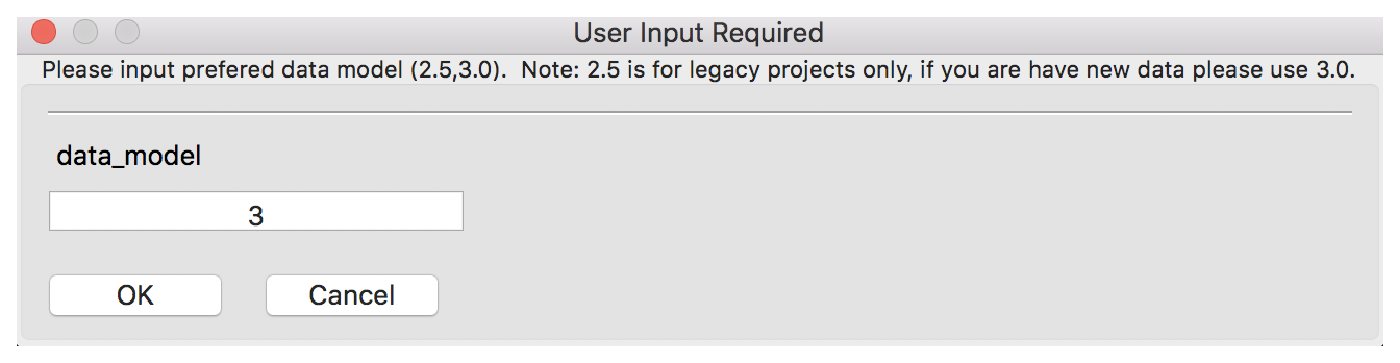
\includegraphics[width=6in]{EPSFiles/PmagGUI_choose_data_model.eps}

\begin{enumerate}
\item Make sure you have followed all of the steps in the \href{#quick_start}{Installing PmagPy} section.

\customlink{Project_Directory}

\item Open your command prompt and start {\bf Pmag GUI} with the appropriate command (pmag\_gui.py, pmag\_gui\_anaconda, or pmag\_gui).  If you are confused about which command to use, see the \href{#finishing_up}{Finishing up} section for details.

\item  When you start {\bf Pmag GUI}, the first step is to change directories into a  `Project Directory'. For each study, create a directory with a name that relates to that study. Here we will call it {\it ThisProject}.  This is where you will collect and process all the rock and paleomagnetic data for a given study, usually a publication. The project directory name should have NO SPACES and be placed on the hard drive in a place that has NO spaces in the path. Under certain Windows versions, this means you should not use your home directory, but create a directory called for example:\begin{verbatim}
  D:\MyPmagProjects\end{verbatim} and put {\it ThisProject} there.
%
%Inside the  {\it ThisProject} directory, create two additional directories: {\it MyFiles} and {\it MagIC}. All the files that you want to convert to the MagIC format should be placed in {\it MyFiles}.  The {\it Project Directory} that {\bf Pmag GUI} seeks is that {\it MagIC} directory.
%
%Your Directory tree might look like this now:
%
%\includegraphics[width=15cm]{EPSFiles/ProjectDirectory.eps}


\item \textbf{copy example files:}  Use \textbf{move\_data\_files.py} to move the  datafiles to an accessible location.  Use: \begin{verbatim}

  move_data_files.py -h\end{verbatim} on the command line for help).  In the {\it data\_files } folder you will find a subfolder named {\it Pmag\_GUI}. Copy the contents of the  \href{#Project_Directory}{\it ThisProject} directory  into  your  own \href{#Project_Directory}{Project Directory} folder.
 \item Start Pmag GUI either by typing {\bf pmag\_gui.py} on your \href{#command_line}{command line}, or (if you have the \href{#standalone}{standalone}), by double-clicking the Pmag GUI icon on your Desktop.
 \item If necessary, change directories by clicking  on the ``change directory'' button and select your own {\it ThisProject} directory.
 \end{enumerate}

 \customlink{convert2magic}

\section{Converting magnetometer files to MagIC format}
\begin{itemize}
\item {\bf Pmag GUI} allows for converting many different laboratory formats.  For more information, see the section on \href{#magnetometer_files}{Supported Rock Magnetometer files}.   In this example, we will use a `generic' file format.
%rshaar% In the {\it MyFiles} folder there are  files containing AF, Thermal, and Thellier measurement data of samples from location Snake River (lava flow site). All samples are from site sr01. The measurement data are arranged in the generic format.
An example of the generic file format is shown here:

\includegraphics[width=30cm]{EPSFiles/FigGenericFormat.eps}

To learn what all the column headers mean look at the documentation for \href{#generic_magic.py}{generic\_magic.py}.

%\item Locate the {\it MyFiles} folder in  the {\it Datafiles} subdirectory named {\it Pmag GUI} and copy the contents to your own {\it MyFiles} directory.
%
%\includegraphics[width=15cm]{EPSFiles/FigMyFiles.eps}

%\item Run the program: Open up a terminal window (Mac) or command prompt (Windows) and type pmag_gui.py on the command line. In the Pmag GUI main panel press the Õchange dirÕ button. Select the MagIC directory in ThisProject when prompted.

\item In your  \href{#Project_Directory}{\it ThisProject} directory  there are three files with AF, Thermal, and Thellier measurement data of specimens from site sr01 (a lava flow site) of \cite{tauxe04b}.  There is also a file with sample orientation, location and other metadata typical for a paleomagnetic study.
\item Press the [Convert magnetometer files to MagIC format] button. If no menu pops up or the window is blank, click on the Python icon  (the little space ship, pencil and paper, or feather) on your dock. You should see a dialog window will appear with different file formats:

\includegraphics[width=30cm]{EPSFiles/FigChooseFile.eps}

\item  Click on  `generic format'  and press the  [import file] button.  A new dialog box will appear. For more details click on the [help] button.
\item  In the dialog box, click on the [Add] button and choose one of the measurements files.
\item  Optional: Insert your EarthRef user name.
\item Choose your experiment type from the dropdown list.

\item Choose specimen-sample naming convention.  In this example, specimen sr01a1 belongs to sample sr01a so the specimen-sample naming convention is  `no. of terminal characters ' and the delimiter/number field is `1' ).
\item Choose sample-site naming convention.  In this example, sample sr01a belongs to site sr01 so the sample-site naming convention is  `no. of terminal characters' with a delimiter/number of  `1'.
\item  Fill in the \href{#MagICDatabase}{EarthRef Location Name}  for this project .  For this project, it is ``Snake River''.
\customlink{location_name}

\item Note:  a location is a stratigraphic section,  a sampling region,  an drill core, and so on.  MagIC doesn't really care what your location name is, but use the same location name every time you are asked for it, because it really ties your dataset together and is required within the data model.

Your dialog boxes should look like this for the AF and thermal data:

\includegraphics[width=30cm]{EPSFiles/FigConvertGenericA.eps}

and like this for the  paleointensity data.  For paleointensity data, you must also supply the lab field in micro tesla (40) and orientation relative to sample's X direction:  0 -90.

\includegraphics[width=30cm]{EPSFiles/FigConvertGenericB.eps}

\item Press OK to create a new MagIC measurement file, which is saved in your \href{#Project_Directory}{\it ThisProject} directory.


\customlink{Combine}

\item After converting all files to MagIC format, press the [Next Step] button in the `convert magnetometer files' dialog box. All files with the .magic suffix will be added to the list.  [You can edit the list by deleting unwanted files or adding additional MagIC formatted files.]   You should see a list of the three magic files:

\includegraphics[width=30cm]{EPSFiles/FigCombineMagic.eps}

\item Click the OK button. The three files will be combined to a single file,  named {\it measurements.txt} and also stored  in your \href{#Project_Directory}{\it ThisProject} directory.

\item In the next dialog, you will combine specimen, sample, site, and location files.
\end{itemize}

\customlink{orient}

\section{Optional: Calculate geographic / tilt-corrected direction}
\begin{itemize}
\item {\bf Pmag GUI} provides an optional tool for calculating geographic and tilt-corrected directions if those directions were not part of the original data files. To use this tool click on the button labeled `calculate geographic/tilt-corrected directions'.

\item When you open this window, an empty template of a file named demag\_orient.txt was created in your project directory. This file is displayed in a Python window. You can fill in  this file manually using the GUI window or \href{#field_info}{with with a spreadsheet program}. The template is pre-filled with sample names derived from your measurement files, using the naming rules that you chose.
\item To fill in the orientation information, click the button $\rightarrow$ [Import Orientation File] and  choose the file SrExample\_orient.txt from {\it MyFiles} folder.
\item Click the button $\rightarrow$ [Save orientation file].
\item Click the button $\rightarrow$ [Calculate sample orientations].
\item Fill in the [set orientation convention] dialog box like this:

\includegraphics[width=25cm]{EPSFiles/FigDemagOrient.eps}

\begin{itemize}
\item Orientation convention :Pomeroy.
\item Declination correction: Use the IGRF.
\item  Orientation priority: \#1.
\item Put in the number of hours to SUBTRACT from the local time to get to Greenwich Mean Time: -6. [Local time was 6 hours behind GMT for this example.]
\item press the OK button.
\end{itemize}
\item In the [additional required information] dialog window add the additional information:
\end{itemize}

\includegraphics[width=15cm]{EPSFiles/FigOrientMagicCodes.eps}

\section{Filling in metadata}

Filling in metadata is a critical part of building a MagIC Project Directory. The data relevant to this example are arranged in five tables: specimens, samples, sites, locations, ages. To complete the data, click the button, and follow the directions in the help window in order:

\begin{itemize}
\item Step 0: Choose the appropriate headers for each of your tables.  Required headers (or headers already present in your tables) show up in the top box, optional headers in the bottom.  In our example, you won't need to add any additional headers.  Once you have added all needed headers, click the OK button to proceed to the next step.

 \includegraphics[width=30cm]{EPSFiles/FigErMagicStep0.eps}

 \item The next steps contain editable grids.  For many columns, you can edit using drop-down menus that provide \href{http://earthref.org/MAGIC/shortlists.htm}{controlled vocabularies}.  For others, you must manually enter data into the cell.  A single left click will bring up a drop-down menu; a double-left click will call up the cell editor.  With both types of data entry, it is possible to select a single value for the entire column. Simply click on the column label.  If that column has a drop-down menu, you can then click on any cell in the column, the appropriate menu will pop up, and the value you select will propagate throughout the column.  Edits in that column will continue to be global until you select another column to edit or you de-select the column by clicking on the column label again.  If you select a column that does not have a drop-down menu, a text entry dialog will pop up, and the value you provide will be applied to the column.

 \item Step 1: Update the specimens table.  You may not rename specimens, but you may reassign them to a different sample.  It is also possible to add additional samples, using the 'Add new sample' button.  Note that type, lithology, and class columns need not be filled in here.  They will propagate down automatically when you select values at the sample or site level for type, lithology, and class.  In this example, you can just click [Save and continue].

 \includegraphics[width=25cm] {EPSFiles/FigErMagicStep1.eps}

\item Step 2:  Update the samples table.  You may rename samples, or you can reassign them to a different site.  You can also add additional sites using the ``Add a new site`` button.  In this example, you can just click [Save and continue].

 \includegraphics[width=20cm] {EPSFiles/FigErMagicStep2.eps}

\item Step 3: Update the sites table.  You may rename sites, or you can reassign them to a different location.  You can add additional locations using the ``Add a new location'' button.  You must choose a legal entry from the \href{http://earthref.org/MAGIC/shortlists.htm}{controlled vocabularies} for the following headers: ``class'', ``lithology'', ``type''. You may combine more than one controlled vocabulary by making them a colon delimited list.  If you select a value in these categories: class, lithology, type, longitude, or latitude, the values will propagate to the samples table.  In this example,  geologic_classes=Extrusive:Igneous; lithologies=Basaltic Lava; geologic_types=Lava Flow.  You should also add age data: age=2.3, age_unit=Ma.

\includegraphics[width=32cm] {EPSFiles/FigErMagicStep3.eps}


\item Step 4: Update the locations table.  If you have provided site latitudes and longitudes, the columns for beginning and ending latitudes and longitudes should be filled in already. Likewise, ``age_high'', ``age_low'', and ``age_unit'' will be filled with data from the sites table.  You must choose a legal entry from the \href{http://earthref.org/MAGIC/shortlists.htm}{controlled vocabularies} for the  ``location\_type''. In this example: location\_type = outcrop.

\includegraphics[width=32cm] {EPSFiles/FigErMagicStep4.eps}

\item Step 5: Add ages data.  For this tutorial, you can skip this step (just press [Save and continue]).

\end{itemize}

\customlink{DemagGUI}

\section{Demag GUI quick start}
\label{sect:demag_gui}

Next, click the [Demag GUI] button.  This is the main panel of the demag GUI:

\includegraphics[width=30cm]{EPSFiles/demag_gui.eps}

Use of the Demag GUI is described in more detail in the \href{#demag_gui.py}{Demag GUI} section below. Here are a few instructions that can be used as a quick start for using Demag GUI. {\bf Note}: If at any point you require help with a particular aspect of Demag GUI clicking on [Help] $\rightarrow$ [Usage and Tips] (hotkey: ctrl-h) then clicking on the item you wish to know more about will provide a pop-up box with information for most all aspects of the GUI and Interpretation Editor, see \hyperref[add-help]{additional help} for details.

Before you start your analysis, you can choose your coordinate system.  From the `coordinate system' drop-down menu you can choose the coordinate system in which you wish to view the data (e.g.  `geographic'). The coordinate system and the orientation of the projection can be switched throughout your analysis which updates the view of the data within the Zijderveld vector component plot and the equal area directional projections.

To analyze the data in the example, follow these steps for each specimen:
\begin{itemize}
\item Click `add a fit' (hotkey: ctrl-n) and choose the temperature/AF bounds for the fit by double clicking on the measurement lines, by double clicking on the measurement points in the Zijderveld plot, or by choosing from the `bounds' dropdown menu.
\item Click the `next' button to analyze the next specimen (hotkey: ctrl-right).
\end{itemize}

To calculate  Fisher mean for the site: choose from the `mean options' drop-down menus.  First select: component=All, then select: mean=Fisher.

All of the fits can be viewed and modified using the Interpretation Editor which can be selected from the Tools menu in the top menubar. (hotkey: ctrl-e)

To permanently save all of the specimen interpretations, choose from the menubar [File] $\rightarrow$ [Save MagIC  tables]. This saves all the interpretations in specimen/sample/site tables in your \href{#Project_Directory}{\it ThisProject} directory. Fits that are saved this way will be loaded into demag\_gui the next time it is launched.  Click through the dialog boxes and fill out choices for generating MagIC results.

If you are partway through your analysis, you may want to save your place without outputting to MagIC tables.  To save temporary analysis data use [File] $\rightarrow$ [Save interpretations to a redo file]. This saves all interpretation data to a redo file which will not load immediately when the GUI starts, but preserves aesthetic aspects of interpretations such as color as well as the specimen you were on when you saved to keep your place in analysis and allows rebooting of session without full export of MagIC tables.

Close the Demag GUI.


\customlink{ThellierGUI}

\section{Thellier GUI quick start}
Next, click the [Thellier GUI] button.  This is the main panel of the thellier GUI:

This image shows the main panel of \href{#ThellierGUI}{Thellier GUI}:

\includegraphics[width=30cm]{EPSFiles/FigThellierGui.eps}

Use of the Thellier GUI is described in more detail in the \href{#thellier_GUI.py}{Thellier GUI} section below and in this PDF document: \href{https://github.com/PmagPy/PmagPy-Cookbook/blob/gh-pages/thellier_GUI_full_manual.pdf}{Thellier GUI manual}. Here are a few instructions that can be used as a quick start for using Thellier GUI.

You can customize which selection criteria you need  under Preferences $=>$ Specimen paleointensity statistics (from SPD list).  This uses the \cite{paterson14} definitions of paleointensity statistices.
Next, select bounds for the statistics under [Analysis] $=>$[Acceptance criteria] $=>$ [Change acceptance criteria].

The default of the program is to calculate sample means. To change it to site level mean, choose from the menubar: [Analysis] $\rightarrow$ [Acceptance criteria] $\rightarrow$  [Change acceptance criteria]. Find the `average by sample/site' dropdown menu in the third row and change it to [site]. Click OK. The site mean will appear in the sample/site results box (top right).

Then, to analyze the data, follow these steps for each specimen:
 \begin{itemize}
 \item Choose temperature bounds from the temperatures dropdown menus.
 \item  Click the ‘next’ button to analyze the next specimen.
   \end{itemize}
Next, you will save these interpretations to a file.  To do so, choose from the menubar [File] $\rightarrow$ [Save MagIC pmag tables]. This save all the interpretations in the specimens.txt file in your MagIC Project Directory.
Close the Thellier GUI.


\customlink{magic_upload}

\section{Upload to the database }

To create a MagIC-format file for upload, you first click on the green {\it Create MagIC txt file for upload} button on the main page of {\bf Pmag GUI}. A file will be created in your \href{#Project_Directory}{\it ThisProject} directory.  Now, go to the  \href{http://earthref.org/MAGIC/}{MagIC  interface}.      Click on the `Upload Tool' button and upload your file by  draging and droping the {\it upload}   file onto the  `Drop and drop files here to upload' window.
Congratulations. Your data are now in the database under a Private Contribution.  But, they are not yet activated and cannot be until they are at least accepted for publication.  After you have a suitable reference, you can Activate your contribution.  Once you activate an uploaded dataset (only for published papers), it will be publicly available.

\customlink{magic_download}

\section{Downloading data from {\bf MagIC}}

Data can be downloaded from the {\bf MagIC} database and examined with {\bf PmagPy} tools.   The \href{http://earthref.org/MAGIC/search/}{\bf MagIC} search interface provides a rich variety of search filters available by clicking on the `Filter the MagIC Search Results' text box.    To locate data from a particular reference,  simply substitute the digital object identifier (DOI) in your browser window:

\href{http://earthref.org/MAGIC/doi/10.1029/2003GC000661}{http://earthref.org/MAGIC/doi/10.1029/2003GC000661}

\noindent The above DOI will find the data for the paper by \cite{tauxe04b}.  [This may fail in Safari; if so, use an alternative browser like Firefox or Chrome.]     To download the data, simply click on the file icon labeled ``Download''.  This will save a file to your downloads folder.
 To unpack this file after downloading it from the database, open \href{#pmag_gui.py}{Pmag GUI} and click ``unpack downloaded txt file``.


 \section{Preparing for MagIC}

\customlink{field_info}

\subsection{Field and sampling information}

 There is an astounding number of different ways that paleomagnetists document data in the field and in the lab. This variety is met with a large number  of method codes that describe sampling and orientation procedures (see \url{https://earthref.org/MagIC/method-codes} for a complete description).   The MagIC database expects sample orientations to be the azimuth and plunge of the fiducial arrow used for measurement (see  \href{http://earthref.org/MAGIC/books/Tauxe/Essentials/WebBook3ch2.html#ch2}{[Essentials, Chapter 9]} )  and the orientation of the bedding to be dip direction and downward dip so no matter what your own preference is, it must be translated into the standard MagIC convention for use with the PmagPy programs and with \href{#pmag_gui.py}{Pmag GUI}.

\href{#pmag_gui.py}{Pmag GUI}  supports two different ways of getting orientation and other sampling related information into a MagIC usable format.  The first way is through \href{#orient}{step 2 on the GUI front panel} and filling in the data from within the GUI.  That way will work for many applications, but it may be desirable to fill the spreadsheet in separately from the GUI by using  a tab delimited file (orient.txt format).   By clicking on  \href{#orient}{step 2 on the GUI front panel}  you create a file named {\it demag\_orient.txt}  which has all of your sample names in it.   Each {\it orient.txt} file should  have all the information for a single location {\it sensu MagIC}.


  \includegraphics[width=15cm]{EPSFiles/orient.eps}

 The next row has the names of the columns.  The required columns are:  sample\_name, mag\_azimuth, field\_dip, date, lat, long, sample\_lithology, sample\_type, sample\_class) but there are a number of other possible columns (e.g., Optional Fields in orient.txt formatted files are: [date, shadow\_angle, hhmm], date, stratigraphic\_height, [bedding\_dip\_direction, bedding\_dip], [image\_name, image\_look, image\_photographer], participants, method\_codes, site\_name, and site\_description, GPS\_Az]).  Column names in brackets must be supplied together and the data for stratigraphic\_height are in meters.  Also note that if these are unoriented samples, just set mag\_azimuth and field\_dip to 0.

% If there is a simple  and consistent relationship between the site name and the sample name (e.g., sample ns034a belongs to site ns034), you do not need to specify a site name here as it will be parsed by \href{#orientation_magic.py}{orientation\_magic.py} when it gets converted  to the MagIC format.  However, many investigators have no such consistent naming scheme.  Moreover, in some cases,  groups of samples or initial site designations need to be re-grouped for averaging.  For example, if it becomes clear that a sequence of lava flows were erupted over a short period of time and should be averaged together, you would need a new site name for all the samples.  Note that there are different understandings of the term {\bf site} in the paleomagnetic community.  We adhere to the MagIC definition of ``site'', which is:
% \begin{quote}
%site: a group of samples that are homogeneous with respect to the property being measured.
%\end{quote}
%\noindent When a site  has no simple relationship to the sample names, a column named  site\_name in the {\it orient.txt} file can be used  with the site name filled in for every sample.

   It is handy  to document the lithology, type and material classification information required by MagIC. These  are all controlled vocabularies listed at \url{http://earthref.org/MAGIC/shortlists.htm}.   For archaeological materials, set the lithology to ``Not Specified''.

   Put in stratigraphic height, sun compass, differential GPS orientation information under the appropriate column headings.  You can also flag a particular sample orientation as suspect, by having a column 'sample\_flag' and setting it to either 'g' for good or 'b' for bad.  Other options include documenting digital field photograph names and who was involved with the sampling.

 For Sun Compass measurements, supply the shadow\_angle, date and time. The date must be in mm/dd/yy format. If you enter the time in local time, be sure you know the offset to Universal Time as you will have to supply that when you import the file. Also, only put data from one time zone in a single file. The shadow angle should follow the convention shown in this figure (from Tauxe et al., 2010): \nocite{tauxe10}

  \includegraphics[width=15cm]{EPSFiles/suncomp.eps}

  \customlink{orientation_schemes}

{\bf Supported sample orientation schemes:}

  There are options for
 different orientation conventions (drill direction with the Pomeroy orientation device  [drill azimuth and hade] is the default), different naming conventions and a choice of whether to automatically calculate the IGRF value for magnetic declination correction, supply your own or ignore the correction.  The program generates {\it er\_samples.txt} and {er\_sites.txt} files.  Be warned that existing files with these names will be overwritten.

 All images, for example outcrop photos are supplied as a separate zip file. image\_name is the name of the picture you will import, image\_look is the ``look direction`` and image\_photographer is the person who took the picture. This information will be put in a file named er\_images.txt and will ultimately be read into the er\_image table in the console where additional information must be entered (keywords, etc.).

Often, paleomagnetists note when a sample orientation is suspect in the field. To indicate that a particular sample may have an uncertainty in its orientation that is greater than about 5$^{\circ}$, enter SO-GT5 in the method\_codes column and any other special codes pertaining to a particular sample from the method codes table. Other general method codes can be entered later. Note that unlike date and sample\_class, the method codes entered in orient.txt pertain only to the sample on the same line.

Samples are oriented in the field with a ``field arrow`` and measured in the laboratory with a ``lab arrow``. The lab arrow is the positive X direction of the right handed coordinate system of the specimen measurements. The lab and field arrows may not be the same. In the MagIC database, we require the orientation (azimuth and plunge) of the X direction of the measurements (lab arrow). Here are some popular conventions that convert the field arrow azimuth (mag\_azimuth in the orient.txt file) and dip (field\_dip in orient.txt) to the azimuth and plunge of the laboratory arrow (sample\_azimuth and sample\_dip in er\_samples.txt). The two angles, mag\_azimuth and field\_dip are explained below.

{\parindent 0pt
[1] Standard Pomeroy convention of azimuth and hade (degrees from vertical down) of the drill direction (field arrow). sample\_azimuth = mag\_azimuth; sample\_dip =-field\_dip.

  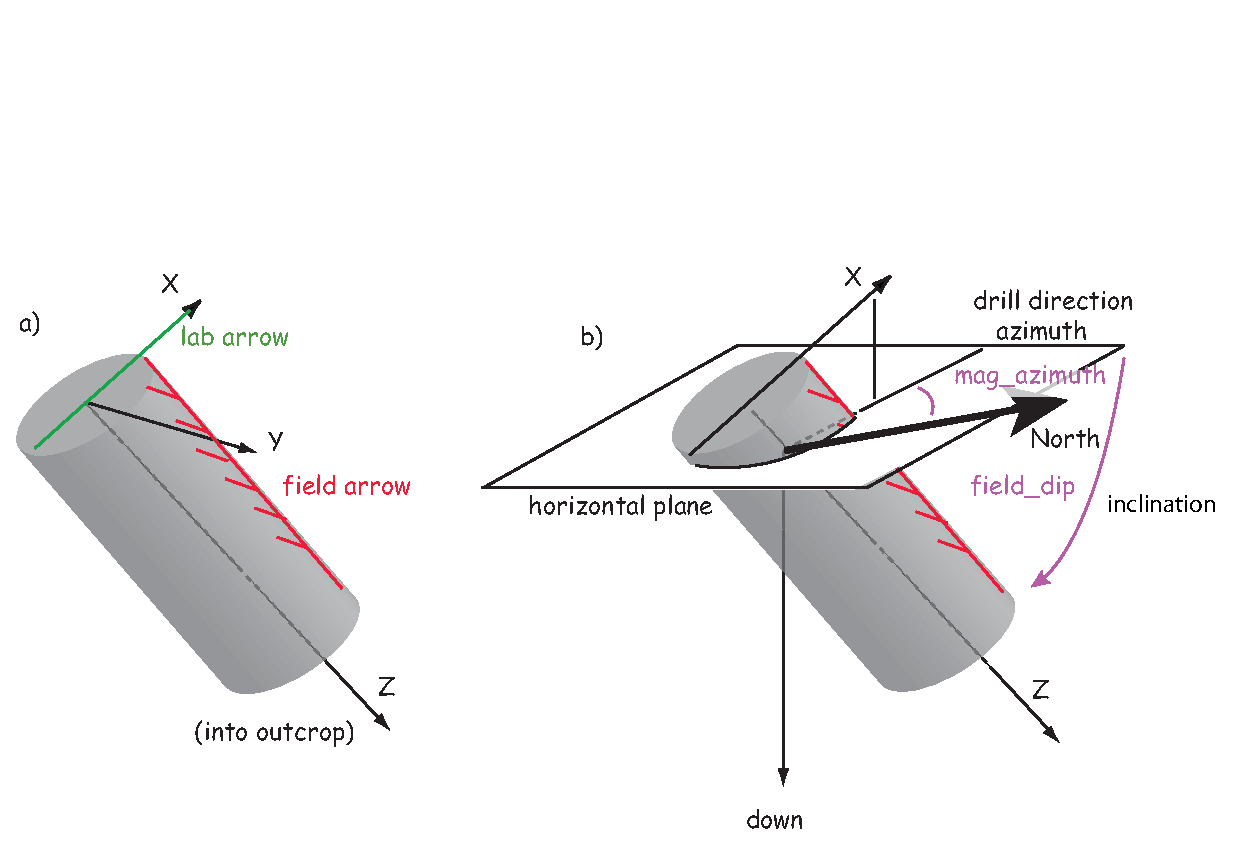
\includegraphics[width=15cm]{EPSFiles/orcon_1.eps}

  2] Field arrow is the strike of the plane orthogonal to the drill direction, Field dip is the hade of the drill direction. Lab arrow azimuth = mag\_azimuth-90$^{\circ}$; Lab arrow dip = -field\_dip

    \includegraphics[width=15cm]{EPSFiles/orcon_2.eps}

  [3] Lab arrow is the same as the drill direction; hade was measured in the field. Lab arrow azimuth = mag\_azimuth; Lab arrow dip = 90$^{\circ}$-field\_dip.

      \includegraphics[width=15cm]{EPSFiles/orcon_3.eps}

  [4] Lab arrow orientation same as mag\_azimuth and field\_dip.

        \includegraphics[width=15cm]{EPSFiles/orcon_4.eps}

        [5]  Lab arrow azimuth is  mag\_azimuth and lab arrow dip is the  field\_dip-90$^{\circ}$

               \includegraphics[width=15cm]{EPSFiles/orcon_5.eps}


 [6] Lab arrow azimuth is mag\_azimuth-90$^{\circ}$, Lab arrow dip is 90$^{\circ}$-field\_dip, i.e., the field arrow was strike and dip of orthogonal face:

                \includegraphics[width=15cm]{EPSFiles/orcon_6.eps}
                }

{\bf Structural correction conventions:}


Because of the ambiguity of strike and dip, the MagIC database uses the dip direction and dip where dip is positive from 0 $\rightarrow$ 180. Dips$ > $90 are overturned beds.


 \customlink{naming_schemes}

{\bf Supported sample naming schemes:}

\begin{verbatim}
            [1] XXXXY: where XXXX is an arbitrary length site designation and Y
                is the single character sample designation.  e.g., TG001a is the
                first sample from site TG001.    [default]
            [2] XXXX-YY: YY sample from site XXXX (XXX, YY of arbitary length)
            [3] XXXX.YY: YY sample from site XXXX (XXX, YY of arbitary length)
            [4-Z] XXXX[YYY]:  YYY is sample designation with Z characters from site XXX
            [5] site name = sample name
            [6] site name entered in site_name column in the orient.txt format input file
            [7-Z] [XXX]YYY:  XXX is site designation with Z characters from samples  XXXYYY
\end{verbatim}

When you are finished with editing the {\it orient.txt} file,  return to  \href{#orient}{step 2 on the GUI front panel}.


%
\customlink{AZDIP}
%
%\subsubsection{AZDIP formatted files}
%
%This is a very simple file format with the sample name Azimuth Plunge Strike Dip where the Azimuth and Plunge are of the drill direction (Specimen's Z direction) or orientation convention \#3 above to convert to the MagIC standard. To convert strike to bedding dip direction, we would just add 90$^{\circ}$. Here is an example AzDip file:
%
%\includegraphics[width=15cm]{EPSFiles/azdip.eps}

\customlink{LIMS}

\subsubsection{Data files downloaded from the IODP (LIMS) database}


There are two types of files that help in plotting of IODP paleomagnetic data sets: the core summaries with depth to core top information and the sample information that contains lists of samples taken.
Visiting the IODP science query website at \url{http://web.iodp.tamu.edu/WTR/html/sci-data.html} allows you to
select 'SRM - Remanence of magnetization' under the Analysis scroll down menu.  By picking the expedition, site, hole, etc. you can download a  .csv format (comma separated values) for the expedition data.  (Be aware that this is the rawest form of the data, including disturbed intervals, bad measurements, core ends, etc. and may not be exactly what ended up getting published!).   First click on the ``Show Report`` button, then, ``Expand Table'', then ``Get File'':

\includegraphics[width=15cm]{EPSFiles/WebTabular_srm.eps}

This can take a very long time, so get yourself a cup of tea.

You can also (while you're at it) click on the 'Summaries' tab and download the coring summaries:

\includegraphics[width=15cm]{EPSFiles/WebTabular_core.eps}

Place both of the downloaded files in your {\it MyFiles} directory.


\customlink{magnetometer_files}

\subsection{Supported Rock Magnetometer files}

The MagIC database is designed to accept data from a wide variety of paleomagnetic and rock magnetic experiments. Because of this the magic\_measurements table is complicated. Each measurement only makes sense in the context of what happened to the specimen before measurement and under what conditions the measurement was made (temperature, frequency, applied field, specimen orientation, etc). Also, there are many different kinds of instruments in common use, including rock magnetometers, susceptibility meters, Curie balances, vibrating sample and alternating gradient force magnetometers, and so on. We have made an effort to write translation programs for the most popular instrument and file formats and continue to add new supported formats as the opportunity arises. Here we describe the various supported data types and tell you how to prepare your files for importing. In general, all files for importing should be placed in the MyFiles directory or in subdirectories therein as needed.  If you don't see your data type in this list, please send an example file and a request to:  ltauxe@ucsd.edu and we'll get it in there for you.


The supported file formats are:

{\bf Rock Magnetometer Files:}

\begin{itemize}
%\item \href{#2G_magic.py}{2G binary format}
\item \href{#cit_magic.py}{The CalTech format used by labs in the RAPID consortium}
%\item \href{#FIN_magic.py}{whatever}
%\item \href{#FLA_magic.py}{Univ. Florida, Gainesville format}
\item \href{#huji_magic.py}{Hebrew University, Jerusalem format}
\item \href{#sio_magic.py}{Scripps Institution of Oceanography format}
\item \href{#ldeo_magic.py}{Lamont Doherty Earth Observatory format}
%\item \href{#LIVMW_magic.py}{Unviersity of Liverpool, microwave format}
\item \href{#iodp_csv_magic.py}{IODP rock magnetometer (SRM) data downloaded from the LIMS database}
\item \href{#pmd_magic.py}{PMD (ascii) format}
\item \href{#tdt_magic.py}{ThellierTool format}
%\item \href{#UB_magic.py}{University of Barcelona format}
%\item \href{#UCSC}{various UC Santa Cruz formats}
%\item \href{#UMICH_magic.py}{University of Michigan format}
%\item \href{#JR6_magic.py}{University of Rome, JR 6 format}
%\item \href{#UU_magic.py}{University of Utrecht format}
\end{itemize}

\customlink{anisotropy_files}

{\bf Anisotropy of Magnetic Susceptibility files:}

\begin{itemize}
\item \href{#s_magic.py}{The 6 tensor element format (.s)}
\item \href{#KLY4S_magic.py}{LabView program} of Gee et al. 2008 \nocite{gee08}
\item \href{#k15\_magic.py}{15 measurement convention of Tauxe 1998 \nocite{tauxe98}}
%\item \href{#susar4-asc\_magic.py}{SUSAR 4.0 ascii output for Kappabridge}
\item \href{#SUFAR4-asc\_magic.py}{SUFAR 4.0 ascii output for Kappabridge}
\end{itemize}

\customlink{Hysteresis_file_formats}

\subsubsection{Hysteresis file formats}
{\bf Pmag GUI} will import hysteresis data from room temperature  Micromag alternating gradient magnetometers (AGM)  in several different ways.  You can import either hysteresis loops or backfield curves, or you can import whole directories of the same.  In the latter case, the file endings must be either .agm (.AGM) or .irm (.IRM) and the first part of the file must be the specimen name.
 See the documentation for  \href{#agm\_magic.py}{agm\_magic.py} for examples.


Now you've collected together all the files you need, we can start importing them into {\it MagIC} directory with   \href{#convert2magic}{\bf Step 1 in Pmag GUI}.



\customlink{magic_gui.py}

\chapter{MagIC GUI Tutorial}
\label{chap:MagIC GUI}

{\bf MagIC GUI} is a Graphical User Interface written by Lori Jonestrask.  It is meant for efficiently compiling a contribution for uploading to the MagIC database.  MagIC GUI is specifically designed for making a contribution without measurement data; if you ARE including measurement data, we recommend that you use \href{#pmag_gui.py}{Pmag GUI} instead.
MagIC GUI allows you to add data at the location, site, sample, and specimen levels.  You can also add results and ages.  The program uses an Excel-like grid interface for entering and editing data.  Useful features include: pop-up menus with controlled vocabularies, multi-cell pasting from external spreadsheets, and built-in validations for MagIC database requirements.
Note: {\bf magic\_gui.py} uses the current MagIC data model, 3.0.  For working with legacy data in the 2.5 format, you should instead use {\bf magic\_gui2.py}.  The tutorial below was written specifically for the older  {\bf magic\_gui2.py} but will soon be updated with illustrations and instructions from {\bf magic\_gui.py}. The two programs do work almost identically, so the tutorial should still point you in the right direction even if you are working with 3.0 data.


\section{Starting with MagIC GUI}
Start up MagIC GUI.  You'll do this by clicking on the icon (if you downloaded the \href{#standalone}{standalone} version) or entering `magic\_gui.py' on your \href{#command_line}{command line} (if you downloaded the full PmagPy installation).  If you are using Anaconda Python, you will type `magic\_gui\_anaconda' on your \href{#command_line}{command line} instead.

When you first start {\bf magic\_gui.py}, you will change directories into a  `Project Directory'. For each study, create a directory with a name that relates to that study. Here we will call it {\it MyProject}.  This is where you will collect  and process all the rock and paleomagnetic data for a given study, usually a publication.   The project directory name should have NO SPACES and be placed on the hard drive in a place that has NO spaces in the path. Under certain Windows versions, this means you should not use your home directory, but create a directory called for example: D:$\backslash$MyPmagProjects and put {\it MyProject} there.

  \includegraphics[width=25cm]{EPSFiles/MM_main_frame.eps}

\section{MagIC GUI example dataset}
Now we'll walk through a simple data input process, with fake data.
  \begin{itemize}
  \item Start by clicking on `1. add location data'.  Enter location data as seen below. Notice use of the context menu: in most instances, these will provide controlled vocabularies.
    \includegraphics[width=40cm]{EPSFiles/MM_location_grid_with_menu.eps}
  \item You'll notice that some information is not filled in.  First, if you have no outside citations, you can leave `er\_citation\_names' blank and it will be automatically filled in with `This study' after you save this data.  Second, if you will be providing latitude/longitude for sites, then you don't need to provide it at the location level.  The program will extract start and end latitude and longitude from your site data and apply it to each location.
  \item If you want to provide more than the default required information, you may want to add more columns to your grid.  In our case, we'll add in `Country'.  To do this, just click the button `Add additional columns'.  Choose whatever headers you want to add and select `Ok'.

    \includegraphics[width=15cm]{EPSFiles/MM_add_location_headers.eps}

  \item Now you'll have a new column with a new controlled vocabulary.  Find and select `U.S.A.'.  When you're done entering location data, click `Save and close grid'.

  \item Next, we'll add in sites, so start by opening the site grid.  We will have two sites in this dataset, so click the `Add row(s)' button once.  Then, fill in the grid.  For some of the values, both sites will have the same value.  To provide this data more efficiently, click on the column label to edit all values in that column.  If that column has a menu, you can then click anywhere in that column and make a selection for every cell in the column. Once you're done editing the column, click the header again to exit the multiple-cell-edit mode.
  \item For controlled vocabulary columns, like `type', it is possible that you might not be able to find an appropriate value, or you might not know the appropriate value.  In that case, most controlled vocabularies provide a `Not Specified' option, which we will use here.

    \includegraphics[width=40cm]{EPSFiles/MM_site_grid_with_edit_all.eps}

  \item Once you're done adding sites, save and close the site grid, then open the sample grid.
    Enter data as you see below:

    \includegraphics[width=40cm]{EPSFiles/MM_sample_grid.eps}

    All other required data will fill in automatically.  If you don't provide latitude and longitude data for a sample, it will propagate down from the site after you save and close the grid.

  \item For samples, we will add an additional statistic.  Click 'Add additional columns' and select `sample\_int\_sigma' from the 'Headers for interpretation data' column.  Select 'ok' and have a look at your new grid.  You'll notice that the column you selected has been added, as well as two additional columns: `magic\_instrument\_codes' and `magic\_method\_codes++'.  These two columns are required if you are including any interpretation data at the sample level.  Fill in the added columns.  You'll notice that `magic\_method\_codes++' has a drop-down menu.  If you aren't familiar with the MagIC codes system, click `Show method codes' which provides brief explanations for each possible code.

    \includegraphics[width=50cm]{EPSFiles/MM_sample_grid_added_cols.eps}

  \item Save and close the sample grid, then re-open it to see how the data have propagated (re-opening the grid isn't necessary for the program, this is just for you to see what MagIC GUI does automatically).

    \includegraphics[width=50cm]{EPSFiles/MM_sample_grid_propagated_full.eps}

  \item In this example, we won't add data at the specimen level, so we will be skipping step 4.  Adding specimens works just the same as adding samples.

  \item Now open the age grid.  You can assign ages at any level, at multiple levels, or at no level.  For this study, we will add ages at the sample level.  Choose sample as the age level.  Next, you'll need to add in the `age' column.  Fill in the grid as below:

    \includegraphics[width=25cm]{EPSFiles/MM_age_grid.eps}

  \item You'll notice that you can't add or remove rows in this grid.  If you want to add an additional sample, you would need to go back to the sample grid to do so.

  \item The last data step is to put in result information.  You'll need to open the result grid and, for this example, add just one statistic: `vadm'.  Then, fill out the grid:

    \includegraphics[width=45cm]{EPSFiles/MM_result_grid.eps}

  \item For each result, you will add one or more items that the result pertains to.  In this example, one result is a site V[A]DM, and the other is an averaged V[A]DM from both sites.  For now, leave magic\_method\_codes blank for the Averaged V[A]DM result: in a minute we'll see how MagIC GUI catches this error.  Save and close the result grid.

  \item Next, you will create a MagIC format upload file.  Click the final button on the main frame, `prepare upload txt file'.  Depending on the size of your contribution, this can take a minute; with our small example, it should be fairly quick.  After hitting upload, you will see an error message, and the main frame will direct you to the problem.  Validations will check for missing required fields, invalid data, and missing ancestors (for instance, a specimen with no sample).

    \includegraphics[width=25cm]{EPSFiles/MM_validation_mainframe.eps}

    Open the result grid to fix the error.  Click `Show help' for more information about validations.  In this case, it is a simple fix: add method code `LP-PI' to the average V[A]DM result.

    \includegraphics[width=45cm]{EPSFiles/MM_filled_in_result_validation.eps}

  \item Now that you've fixed your error, try `prepare upload txt file' again.  This time there should be no problems, and you are ready to \href{#magic_upload}{upload your data}!

\end{itemize}




%
%
\customlink{MagIC.py}
%
%\chapter{MagIC.py}
%\label{chap:MagIC} \href{#MagICDatabase}{[MagIC}]
%
%While \href{#pmag_gui.py}{Pmag GUI} provides a bare bones interface for importing, interpreting and uploading most demagnetization and paleointensity experimental data into the MagIC database, {\bf MagIC.py} is a more complete (and complicated) program.
%It is an umbrella program that links many MagIC related functions of the \href{#PmagPy}{PmagPy} Software Package in a user-friendly  graphical user interface (GUI).  While it is invoked with a command line call, this  can be done from any directory (with no spaces in the path).  It generates calls to the programs described in Chapter~\ref{chap:PmagPy} so you don't have to.    It allows importing of many lab and instrument formats, plotting of a variety of data and doing the data processing and book-keeping required to create files ready for uploading into the MagIC Console software.




\customlink{survival_skills}

\chapter{Survival computer skills}
\label{ex:unix}

The `Py' part of  `PmagPy' stands for Python, the language in which all the code is written.   It is not essential, but it is helpful, to understand a bit about computer operating systems and the Python language when using PmagPy because no one should be using programs as black boxes without understanding what they are doing. As all the programs are open source, you have the opportunity to look into them.  If you understand a bit about how computers work yourself, you will be able to follow along what the programs are doing and even modify them to work better for you. In this chapter, you will find a brief introduction to the computer skills necessary for using the programs properly.  We have tried to make this tutorial operating system independent.  All the examples should work equally well on Mac OS, Windows and Unix-type operating systems.  For a more complete explanation of the marvelous world of UNIX, refer to the website at \url{http://www.tutorialspoint.com/unix/unix-quick-guide.htm}.  For handy tricks in DOS, try this link:  \url{http://www.c3scripts.com/tutorials/msdos}.
For an introduction to programming in Python, see the \href{#Python}{Python Programming Chapter}.   For now, we are interested in having the skills to find a command line and navigate the file system in order to get started with \href{#PmagPy}{PmagPy}.


\customlink{command_line}
\section{Finding your command line}
If you are not using a Unix-like computer (*NIX), you may never have encountered a command line. Using any of the command line programs requires accessing the command line.  If you are using the MacOS operating system, look for the Terminal application in the Utilities folder within the Applications folder. When the Terminal application is launched, you will get a terminal window. The Unix (and MacOS) Bash shell has a \$ sign as a prompt.  Other shells have other command line prompts, such as the antiquated `C-shell' used by Lisa Tauxe (don't ask) which has a \% prompt which is used in the examples here.

  \includegraphics[width=15cm]{EPSFiles/terminal.eps}

Under the Windows operating system, you can find your command line by searching for the ``Command Prompt'' application.

  \includegraphics[width=15cm]{EPSFiles/cmd.eps}

  Note that the location of this program varies on different computers, so you may have to hunt around a little to find yours. Also, the actual  ``prompt'' will vary for different machines.



\section{File systems}
\label{sect:file_systems}
When you first open a terminal window,  you are in your ``home'' directory.
Fundamental to all operating systems is the concept of
directories and files.  On windows-based operating systems (MacOS or Windows), directories are depicted
as ``folders'' and moving about is accomplished by clicking on the different icons.
In the world of terminal windows, the directories have names and are arranged in a hierarchical sequence with
the top directory being the ``root'' directory, known as  ``/'' (or C:\verb!\! in Windows) and the file system looks something like this:


  \includegraphics[width=15cm]{EPSFiles/filesys.eps}

 Within the root directory, there are subdirectories
(e.g. {\bf Applications} and {\bf Users} in bold face).  In any directory, there can also be ``files''
(e.g. {\it dir\_cart\_example.dat}).   To
refer to directories,  the operating system relies on what is called a ``pathname''. Every object
has an ``absolute'' pathname which is valid from anywhere on the computer.  The
absolute pathname in *NIX always begins from the root directory {\bf /} and in DOS (the operating system working in the Windows command line window), it is C:\verb!\!.

The absolute pathname to the home directory {\bf lisa} in the figure is {\bf /Users/lisa}.
Similarly, the absolute pathname to the directory containing {\bf PmagPy}
scripts  would be  {\bf /Users/lisa/PmagPy}.  There is also a ``relative'' pathname,
which is in reference to the  current directory (the one you are `sitting' in).  If user ``lisa'' is sitting in
her home directory, the relative pathname for the file {\it dir\_cart\_example.dat} in the directory
{\bf data\_files} would be {\it data\_files/dir\_cart/dir\_cart\_example.dat}.  When using relative
pathnames, it is useful to remember that {\bf ./} refers to the current
directory and {\bf ../} refers to the directory  ``above''.     Also, lisa's home directory would be $\sim$lisa, or if you are logged in as lisa yourself, then it is just $\sim$.


\customlink{file_system}
\section{Moving around in the file system}

Now that you have found your command line and are comfortable in your home directory, you can view the contents of your directory with the Unix command {\bf ls} or the DOS command {\bf dir}.
\customlink{mkdir}
You can make a new directory with the command
\begin{verbatim}
% mkdir NEW_DIRECTORY_NAME
\end{verbatim}
This command works in both Unix and DOS environments) and you can move into your new directory with the command
\begin{verbatim}
% cd NEW_DIRECTORY_NAME
\end{verbatim}
   To move back up into the home directory, just type {\bf cd ..} remembering that {\bf ..} refers to the directory above.  Also, {\bf cd} by itself will transport you home from where ever you are (there's no place like home....).     You can also change to any arbitrary directory by specifying the full path of the destination directory.


%\section {Wildcards}
%
%Unix and DOS have the ability to refer to a number of files and/or directories using
%``wildcards''.  The  wildcard for a  single character is ``?'' and for any number of
%characters is ``*''.  For example, to refer to all the files with ``.py'' in their name in the PmagPy directory in my home directory,
%I would type:
%
%\begin{verbatim}
%% ls PmagPy/*.py
%apwp.py bootams.py fishrot.py.....
%\end{verbatim}

\customlink{standard_IO}

\section {Redirecting input and output}

Programs that operate at the command line level print output to the screen and read input
from the keyboard. This is
known as ``standard input and output'' or ``standard I/O''.
One of the nicest things about working at the command line level is the ability to redirect input and output.
For example, instead of typing input to a program with the keyboard, it can
be read from a file using the symbol {\bf $<$}.   Output can either be printed to the screen (standard output), redirected into a file using the symbol {\bf $>$}, appended to the end of a file with {\bf $>>$} or
used as input to another program with the pipe operator ({\bf$ |$}).

\section{Text editors}

There are many ways of editing text and the subject is beyond the scope of this documentation. Text editing is a blessing and a curse.  You either love it or
hate it and in the beginning, and if you are used to programs like Word, you will certainly hate it. (And if you are used to a decent text editor, you will hate Word!).      But you can't use Word because the output is in a weird format that no scripting languages read easily.  So you have to use text editor that will produce a plain (ascii) file, like Notepad, TextWrangler, Sublime Text or Atom.  \href{http://textwrangler.onfreedownload.com}{TextWrangler} is free software available for Macs, the notepad comes standard in the Windows operating system and the \href{https://atom.io}{Atom} text editor is a free cross-platform option with lots of nice packages available that extend its functionality. Enthought Python's Canopy programming environment comes with its own text editor.

\customlink{PmagPy}

\chapter{The {\bf PmagPy} software package}
\label{chap:PmagPy}

The {\bf PmagPy} software package is a comprehensive set of programs for paleomagnetists and rock magnetists.  For installation,  follow the instructions in the \href{#quick_start}{Installing PmagPy} Chapter in this cookbook. \\

\noindent When you type something on your \href{#command_line}{command line}, your operating system looks for programs of the same name in special places.  These are special ``paths'' so the directory with your Python scripts has to ``be in your path''.  To inform the operating system of the new directory, you need to ``set your path''.    It should have been set when you installed {\bf PmagPy}.

\customlink{demag_gui.py}


\section{Graphical data analysis programs}
\subsection{demag\_gui.py}

The  Demag GUI ({\bf demag\_gui.py}) program enables the display and analysis of paleomagnetic demagnetization data. The software will display specimen level data within the chosen directory as a Zijderveld plot, equal area plot and intensity plot. Interpretations can be made to the data as least-squares line or plane fits. Mean directions can be calculated and displayed for these interpretations. These interpretations can be exported as MagIC pmag files from the program.

\subsubsection{Launching}\label{launching}

The best way to launch the Demag GUI application is through  \href{#pmag_gui.py}{Pmag GUI}. If you have installed PmagPy using pip, (or if PmagPy has been added to your PATH), you can type pmag\_gui.py at the command line to launch it.  Anaconda users will instead type `pmag\_gui\_anaconda'.

\noindent Alternatively, you can navigate to the PmagPy home directory  and type \texttt{python  ./pmag\_gui.py}. Within \href{#pmag_gui.py}{Pmag GUI}, data can be converted from the format of a particular lab into MagIC format so that it can be displayed and analyzed within Demag GUI. The program can be started by clicking on the Demag GUI button in \href{#pmag_gui.py}{Pmag GUI}.


\noindent If you want to launch {\bf Demag GUI} directly, (assuming {\bf PmagPy} was properly installed using pip or has been added to your PATH), you can simply type
demag\_gui.py at the command line. Anaconda users will type `demag\_gui\_anaconda' instead.  \textbf{Note:} on OSX it is
recommended to launch through \href{#pmag_gui.py}{Pmag GUI} as on wxpython 2.9 the drop-down boxes behave better when {\bf Demag GUI} is launched this way.\\


\includegraphics[width=10 cm]{EPSFiles/demag_gui_QuickMagicLauncher.eps}

\noindent {\bf Demag GUI} can also be launched through the command line by navigating to the directory containing {\bf demag\_gui.py}  and running it with:\\

\begin{verbatim}
% python ./demag_gui.py
\end{verbatim}


%\begin{verbatim}
% pythonw ./pmag_gui.py
%\end{verbatim}

\subsubsection{Adding and Editing Specimen Interpretations:}\label{adding-interpretations}

A new fit can be added by clicking the `add fit' button or if no fit has yet been created for the current specimen by double clicking on two measurements in the list of measurements to the left or by double clicking on the data points on the zijderveld plot. It is also possible to add interpretations in mass using the \hyperref[interpretation-editor]{interpretation editor} tool described bellow. Additionally, you can select the fit you would like to edit or view by using the drop-down menu under the add fit button. Once you have selected a fit, the shape of the end points of the selected fit will turn to diamond shapes on all plots to distinguish them from the other data points.\\

\includegraphics[width=10 cm]{EPSFiles/demag_gui_Fit.eps}

\noindent Once the desired fit is selected, its bounds can be edited using the drop-down boxes under the bounds header.\\

\includegraphics[width=3 cm]{EPSFiles/demag_gui_BoundsBox.eps}

\noindent Another way to select bounds is to double-click the list of measurement steps in the list on the left. The included steps in the currently selected interpretation are shown in highlighted in blue on the measurement list and the measurements marked ``bad'' are shown in highlighted in red. In the case of duplicate measurements, the first \emph{good} measurement with the same treatment is used as a bound. All points between the selected bounds that are flagged good (i.e. not flagged bad and marked in red), including duplicate measurements, will be included in the interpreted fit.\\

\includegraphics[width=5 cm]{EPSFiles/demag_gui_DataBox.eps}

\noindent Finally, you can select the bounds of an interpretation directly off the Zijderveld plot by hovering your mouse over a measurement (should change to a hand shape) and double clicking.\\

\noindent When first created, the fit will be given a generic name such as
\emph{Fit 1}. The name of the fit can be changed from the default by typing into the drop-down box containing fit name and then pressing enter. The default fit type is a least-squares line. You can choose different fits, such as a line anchored to the origin or a plane, by using the drop-down menu under the label `interpretation type'. Plane fits can be plotted as either poles, full planes, partial planes, best fit vectors, or best fit vectors and full plane ({\bf Note:} plane poles will be displayed as squares and best fit vectors will display as sideways triangles on \hyperref[higher-level-plots-and-interpretation]{high level mean plot}). This display option can be changed in the second drop-down menu under interpretation type.\\

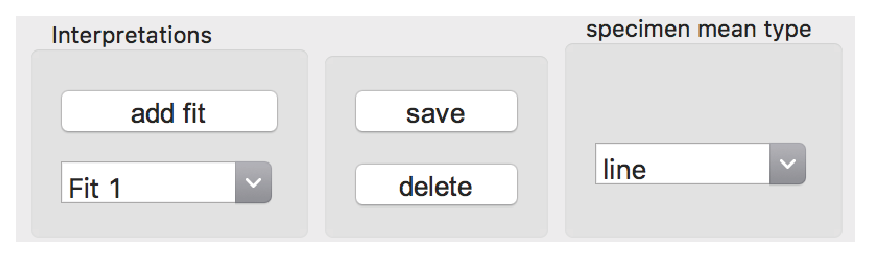
\includegraphics[width=10 cm]{EPSFiles/demag_gui_SpecimenMeanType.eps}

\noindent The properties of the currently selected fit to the data can be seen in the upper center of the GUI in a box labeled `Interpretation Directions and Statistics'.\\

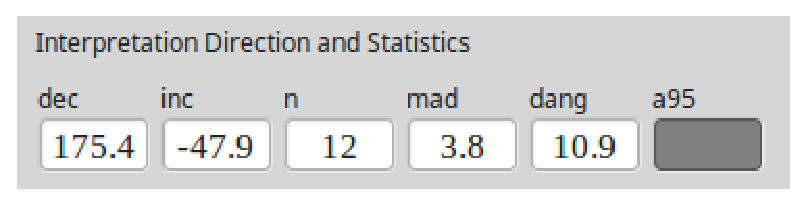
\includegraphics[width=10 cm]{EPSFiles/demag_gui_FitData.eps}

\subsubsection{Deleting Specimen
Interpretations}\label{deleting-specimen-interpretations}

\noindent If you would like to delete a single interpretation, select the one you wish to delete from the interpretation drop-down menu and click delete. If you wish to clear all interpretations you may go into the \hyperref[interpretation-editor]{interpretation editor} located under the tools menu, select the fits you wish to delete and click the ``delete selected'' button.\\

\subsubsection{Changing Specimen, Coordinate System, and Zijderveld Direction:}\label{change-specimen-coord-zijd}

You can switch current specimen by clicking the next or previous button under the specimen box in the side bar (hotkey: ctrl-right and ctrl-left respectively). You can also select specimen from the drop-down menu or type the name of the specimen directly into the specimen box and hit enter to go directly to that specimen. Finally, you can double click on any of the points on the higher level means plot to switch directly to that specimen and interpretation.

\noindent The choice between coordinate systems (i.e.~specimen, geographic or tilt-corrected) is available on the left above the list of steps. The data list and the plots will update to reflect the chosen coordinate system.

\noindent You can alter the X axis of the Zijderveld plot using the Zijderveld plot interactions box to set X=North, East, or NRM dec.

\includegraphics[width=5 cm]{EPSFiles/demag_gui_ProjectionChoice.eps}

\subsubsection{Flagging Bad Measurement
Data}\label{flagging-bad-measurement-data}

Due to flux jumps or other such errors, individual measurements should sometimes be excluded from interpretation. Such measurements can be flagged as ``bad'' by right clicking them within the measurement list and the measurement will then be highlighted in red. Additionally, you can double right click on the point you want to make bad in the Zijderveld plot to toggle it bad. The measurement\_flag in the magic\_measurements file will be change from ``g'' to ``b'' when a measurement is marked as bad the step will not be included in fits that are made to the data. Any measurement marked as bad will be colored red in the step list and will be shown as an empty rather than filled circle on the Zijderveld, equal area and M/M\_0 plots. To change a bad measurement back to being good, one can right click on it again. Upon doing so, the red highlighting will go away, the data will be shown colored in within the plots and any fit that spans that data point will be recalculated to include it.

\noindent Acceptance criteria can be set by using the menu option [Analysis] $\rightarrow$ [Acceptance
Criteria] $\rightarrow$ [Change Acceptance Criteria]. These criteria will be written to a {\it pmag\_criteria.txt}  table. These criteria can then be used to exclude interpretations that fail checks against this criteria during export.

\subsubsection{Plot Interface}\label{plot-interface}

The four plots that take up the majority of the center of the GUI are where data and their interpretations are displayed. All plots are initially set to zoom mode and this is signified by a cross shaped cursor when you mouse over them. To zoom simply click and drag the rectangle to the desired area. You can switch to pan mode by right clicking on any one of the graphs and then clicking and dragging will pan around the plot. Finally, to return to the original plot zoom level and position simply click the middle mouse button to return home. \textbf{Note:} In the absence of a middle mouse button pressing both right and left mouse buttons at the same time works on most laptops in the case of Macbooks clicking with two fingers should work, and if using Apple's magic mouse we recommend you download the \href{http://magicprefs.com/}{MagicPrefs} program which will allow you to configure your mouse however you prefer.

\noindent On the Zijderveld plot you have the additional option to select the current interpretation's bounds by double clicking on a measurement point. You can also double right click on a measurement point in the zijderveld plot to mark it bad.

\noindent On the equal area plots, both the specimen and high level means, you can double click on any interpretation to switch to that specimen and interpretation immediately.

\subsubsection{Saving Specimen Interpretations}\label{saving-specimen-interpretations}

Once you have picked out your interpretations, you can save the session data in two different ways: (1) as a .redo file which will allow you to have the fits preserved to be view again with Demag GUI or (2) as MagIC {\it pmag\_*} tables to be uploaded to the MagIC database or otherwise processed. In addition, you may save image files of the plots.

\paragraph{The .redo File:}\label{the-.redo-file} You can use the menu option [File] $\rightarrow$ [Save current interpretations to a redo file] to create this file type, you can just click the save button next to add fit, or you can use the hotkey ctrl-s. The advantage of the .redo file type being that it is designed to save your place when analysing a large dataset. Loading a redo file will reload all interpretations previously created any special colors assigned to them and take you to the specimen you saved the redo file on allowing you to pick up where you left off. \textbf{Note:} This file type does \textbf{NOT} load previous interpretations on start up you must go to the menu option [File] $\rightarrow$ [Import previous interpretations from a redo file] (hotkey: ctrl-r) to restore your previous session.

\paragraph{The Pmag Tables:}\label{the-pmag-tables} By going to the menu [File] $\rightarrow$ [Save MagIC pmag tables] you can export your interpretations made in Demag GUI to the MagIC pmag tables which can then be used by other MagIC programs or uploaded to the MagIC database. You can export any or all of the three coordinate systems upon selecting this option and you may choose to save {\it pmag\_samples, pmag\_sites}, and {\it pmag\_results}  tables in addition to the {\it pmag\_specimens } table that is output. If you choose to output additional information you will be prompted by a pop up window for additional information. \textbf{Note:} This save format loads on start up of the GUI immediately restoring your interpretations. Selection of this option will overwrite your {\it demag\_gui.redo} file in the working directory.

\paragraph{Images of Plots:}\label{images-of-plots} Select the menu option [File] $\rightarrow$ [Save plot] $\rightarrow$ [Save all plots] to save all plots, or you can save any of the plots individually. If you zoom or pan any of the plots the shifted image will be saved not the originally plotted image although the plot will redraw and reset to the original image in the GUI.

\subsubsection{Flag Specimen Interpretations Good or Bad}\label{flag-spec-interps}

You can flag the current specimen interpretation (marked by large diamonds on all plots) good or bad by using the menu option [Analysis] $\rightarrow$ [Flag Interpretations]. The list of interpretations in the \hyperref[interpretation-editor]{interpretation editor} tool of Demag GUI can also be used to toggle interpretations good or bad in the same way that measurements can be marked good or bad in the measurement list, by right clicking on the entry you want toggled. This will change the shape of the interpretation to a small diamond on all plots, remove it from use in any higher level means, and mark the entry specimen_flag in the pmag tables b instead of g to signify this.

\subsubsection{Sample Orientation}\label{sample-orient}

You can check sample orientation by using the menu option [Analysis] $\rightarrow$ [Sample Orientation] $\rightarrow$ [Check Sample Orientations] (hotkey: ctrl-o). This function will set your mean options to fisher of all components at the current site level and display the wrong arrow (up triangle), wrong compass (down triangle), and rotated sample for declanation incraments of 5 degrees (dotted circle). This allows you to check if the sample orientation is correct and thus can be used in analysis. If you determine the current sample orientation to be bad you can mark it as such using the menu option [Analysis] $\rightarrow$ [Sample Orientation] $\rightarrow$ [Mark Sample Bad] (hotkey: ctrl-.). This will change the sample_orientation_flag in the er_samples file to b not g and will prevent you from marking the specimen interpretations good in that sample so you do not use the improperly oriented data in your final results. If you later realize this was a mistake you can mark the sample orientation good again using [Analysis] $\rightarrow$ [Sample Orientation] $\rightarrow$ [Mark Sample Good] (hotkey: ctrl-,). Finally, to turn off the check sample orientations data simply select the [Check Sample Orientations] option again and it will be removed. \textbf{Note:} The current sample is specified as the sample of the current specimen.

\includegraphics[width=10 cm]{EPSFiles/demag_gui_CheckSampleOrient.eps}

\subsubsection{High Level Means Plot and
Statistics}\label{higher-level-plots-and-interpretation}

The set of drop-down boxes to the right of the interpretation data are there to determine what level you want to analyse in the high level means plot and are grouped into the Display Level and Mean Options boxes.

\includegraphics[width=8 cm]{EPSFiles/demag_gui_HighLevel.eps}

\noindent The Display Level boxes consist of the upper drop-down menu which allows you to select the level at which interpretations are displayed options being all interpretations in the current: sample, site, location, or study. The lower drop-down menu lets you select what the current sample, site, location, or study is.

\noindent The top drop-down menu in the Mean Options box lets you chose what kind of mean you would like to take of the specimen components currently displayed. The lower drop-down menu lets you pick which specimen components to display allowing you to display All components, No components, or any single component.

\noindent The mean statistics for the chosen high level mean are displayed in the lower right of the GUI and can be cycled through using the arrow buttons next to the statistics boxes in the case of multiple high level means.

\noindent It is possible to toggle on and off displaying any one of the means in the high level plot which can be useful in the case of a cluttered graph of all components. This can be done by going to the menu option [Analysis] $\rightarrow$ [Toggle Mean Display] and selecting the name of the component you would like to toggle.

\noindent All interpretations marked bad will appear as small diamonds regardless of type on the high level mean plot. The below gives examples for a number of plane display options of bad interpretations (the symbols off to the side), best fit vectors to the means (sideways triangles), plane poles (squares), and the planes themselves.

\includegraphics[width=30 cm]{EPSFiles/demag_gui_HLMTypes.eps}

\subsubsection{Interpretation Editor}\label{interpretation-editor} %Make this a lot larger

In order to more easily view and edit specimen interpretation data there is a specimen interpretation editor which can be launched using the menu option [Tools] $\rightarrow$ [Interpretation Editor] (hotkey: ctrl-e). \textbf{Note:} If you would like more help than provided here the interpretation editor has in context help same as the main GUI, see \hyperref[add-help]{additional help} for details.
\paragraph{List of Interpretations:}\label{IE-list} This panel contains a list which details the fits made to the data and their parameters from which you can select which interpretation to view by double clicking it. In the list, the currently selected interpretation is highlighted blue as shown in the image below. You can mark interpretations as bad which removes them from any Fisher means or other high level means by right clicking on their entry in the list. All interpretations marked bad are colored red in the list and marked as a small diamond on the plot. The specimen entry associated with this fit will be given a bad (`b') flag within the pmag\_specimens table. You can search through interpretations by using the search bar above the list. Finally, interpretations can be highlighted by clicking on the list and holding the shift or ctrl/command key to select multiple interpretations.
\paragraph{Buttons and Boxes:}\label{IE-buttons} Highlighting entries allows you to delete or alter the characteristics of multiple interpretations at once without having to select each one in turn. This mass alteration is allowable using the the Name/Color/Bounds boxes to input the changes and then clicking the ``apply changes to highlighted fits'' button. You can delete highlighted fits using the ``delete highlighted fits'' button. The ``add fit to highlighted specimens'' button in the interpretation editor adds a fit to all highlighted specimens in the list on the left. You can use the ``add new fit to all specimens`` as a convenient option to add a new interpretation with all the attributes described in the above Name/Color/Bounds boxes to every specimen with measurement data. This is a useful method for quickly analysing a new dataset by checking for components between common unblocking steps like giving every specimen a general magnetite interpretation inferring about where that should be (e.g. bounds=300C to 580C, name=MAG, color=violet).
\paragraph{Additional High Level Means Options:}\label{IE-HLM-options} The interpretation editor also allows the displaying of site and sample means as the primary points on the high level mean plot by changing the bottom left display options drop-down box. Though it does not yet allow taking fisher means of sample means or site means so the mean type box will be forced to read ''None'' if this option is changed from specimens.

\includegraphics[width=15 cm]{EPSFiles/demag_gui_InterpEditor.eps}

\subsubsection{VGP Viewer}\label{vgp-view}

Another tool offered by Demag GUI is the VGP (Virtual Geomagnetic Pole) Viewer which allows you to view your VGPs before exporting to MagIC tables. This tool can be opened by using the menu option [Tools] $\rightarrow$ [View VGPs] (hotkey: ctrl-shift-v). The VGP viewer requires latitude and longitude data for sites and locations in order to calculate all VGPs from specimen interpretations, if this data is not already contained in the MagIC tables imported when the GUI started then it will be asked for during calculation so have it ready. The VGP viewer allows you to select viewing samples, sites, or location VGPs from the drop-down menu at the top. Plot interactions are the same here as in the main GUI and can be zoomed, panned, and points selected in the same manner. The list on the left shows all the data for the currently displayed VGPs.

\includegraphics[width=15 cm]{EPSFiles/demag_gui_VGPViewer.eps}

\subsubsection{Current Warnings Box}\label{warn-box}

The white box in the far top right of the GUI is there to provide relevant warnings about aspects of the current specimen and interpretation such as missing data or duplicate data and can be useful in debugging and analysis.

\subsubsection{Additional Help}\label{add-help}

Finally, if you need more help working with Demag GUI it offers in context assistance with the menu option [Help] $\rightarrow$ [Usage and Tips] (hotkey: ctrl-h) which will change your cursor and then let you click on whichever aspect of the GUI you want help with. Once you have clicked a yellow pop-up box with information should appear in most cases, not all features have information but most should.

\includegraphics[width=10 cm]{EPSFiles/demag_gui_ContextHelp.eps}

\customlink{thellier_GUI.py}

\subsection{thellier\_gui.py}
\href{http://earthref.org/MAGIC/books/Tauxe/Essentials/WebBook3ch10.html#ch10}{[Essentials Chapter 10]} and \href{#MagIC}{[MagIC}]
\href{https://github.com/PmagPy/PmagPy-Cookbook/blob/gh-pages/thellier_GUI_full_manual.pdf}{[Thellier\_GUI\_full\_manual.pdf]}

The program Thellier GUI ({\bf thellier\_gui.py})  combines functions from \href{#thellier_magic.py}{thellier\_magic.py} and new tools described by  \href{http://dx.doi.org/10.1002/ggge.20062}{Shaar and Tauxe (2013)} \nocite{shaar13} in a user-friendly graphical user interface (GUI).

As with \href{#demag_gui.py}{Demag GUI}, Thellier GUI can  be called from  the  \href{#command_line}{command line} or from within \href{#pmag_gui.py}{Pmag GUI}.

To launch Thellier GUI independently, find your command line and enter:

\begin{verbatim}
thellier_gui.py
\end{verbatim}

If using Anaconda Python, you will instead use:

\begin{verbatim}
thellier_gui_anaconda
\end{verbatim}

Once open, Thellier GUI loads  files already prepared in a  \href{#ThisProject}{This Project} directory and the interpretations from Thellier GUI are part of the workflow of  \href{#pmag_gui.py}{Pmag GUI}.   This section is a brief introduction on how to use Thellier GUI as a stand alone application. Much more information is available within this manual: \href{https://github.com/PmagPy/PmagPy-Cookbook/blob/gh-pages/thellier_GUI_full_manual.pdf}{Thellier GUI full manual}.

\noindent  A complete list of the definitions for paleointensity statistics used by Thellier GUI is available as a supplement to the article by \href{#http://dx.doi.org/10.1002/2013GC005135}{Paterson et al., 2014}  \nocite{paterson14} and available for download here:

  \url{http://onlinelibrary.wiley.com/store/10.1002/2013GC005135/asset/supinfo/ggge20412-sup-0001-suppinfoCORRECTED.pdf?v=1&s=e1c3ab0a86c942d1039f6d2e15496aa172dc86ec}

\customlink{choose_directory}
After launching the program,  a  ``choose project directory'' dialog window will appear as soon as the GUI is started.
%
%	\includegraphics[width=15cm]{EPSFiles/Screenshot_choose_directory.eps}
%
%
Your  \href{#Project_Directory}{ThisProject} directory should include a file named {\it magic\_measurements.txt} (created for example by \href{#pmag_gui.py}{\bf Pmag GUI}.   If a file named {\it rmag\_anisotropy.txt} is in the project directory, then the program reads in the anisotropy data. Reading and processing the measurements files may take several seconds, depending on the number of the specimens.


\subsubsection{Reading and compiling measurements data}
When your \href{#Project_Directory}{ThisProject}  project directory is selected, the program  reads all the measurement data, checks them, processes them and sorts them. If non-linear-TRM (NLT) data exist in {\it magic\_measurement.txt}  then the program tries to process the data using Equations (1)-(3) in \href{http://dx.doi.org/10.7288/V4/MAGIC/12116}{Shaar et al., 2010}. \nocite{shaar10}  The program reads {\it magic\_measurement.txt}, and processes the measurements for presentation as Arai  and Zijderveld plots.
We recommend that you check all the warnings and errors in {\it Thellier\_GUI.log} before starting to interpret the data.  For details about warnings and error messages during these steps, consult the tutorial document in the {\it thellier\_GUI} folder in  {\it data\_files}.  Also, consult the Preferences to change certain plotting options.

\subsubsection{Main panel}

This figure shows a snapshot of the main panel.

  \includegraphics[width=30cm]{EPSFiles/Screenshot_main_panel.eps}

\noindent
  The top field in the  panel includes the following buttons/controls (from left to right):
  \begin{itemize}
\item {\bf Specimen:} a list of the specimens in the project folder sorted by name.
\item {\bf previous/next:} buttons to move forward and backward in the specimens list.
\item {\bf T min/T max:} buttons to select temperature bounds.
\item {\bf save/delete:} save or delete current interpretation. This information will be used later to generate a \href{#mk_redo.py}{redo file}.
\item {\bf B\_lab:} laboratory field in units of $\mu T$.
\item {\bf B\_anc:} specimen's paleointensity in units of $\mu T$.
\item {\bf Aniso Correction:} anisotropy correction factor.
\item {\bf NLT Correction:} Non-Linear TRM (NLT) correction factor.
\item {\bf Dec/Inc:} Specimen declination/inclination calculated by PCA of the NRM in the selected temperature bounds.
\item Sample mean, number of specimens, standard deviation and percent standard deviation.
\end{itemize}

The center of the main panel has these elements:

\begin{itemize}
\item {\bf measurements text panel:} Four columns of the measurement data: Step is ``N`` for NRM, ``Z`` for zero field step, ``I`` for infield step, ``P`` for pTRM check, and ``T`` for tail check. The temperature of each step is given in C. Also shown  declination, inclination and moment (in units of $Am^2$)
\item {\bf Arai plot:}  Arai plot normalized by $NRM_0$. blue circles are zero field steps, red circles are infield steps, triangles are pTRM checks, blue squares are tail checks. Temperatures are displayed near data points. Temperature bounds and best fit line are marked in green. 'SCAT box' is marked with dashed lines (only if SCAT is True).
\item {\bf Zijderveld plot:}  A Zijderveld plot of the NRM step.  The x axis is rotated to the direction of the NRM, blue is the x-y  projection, and red is x-z projection.
\item {\bf Equal area plot:}  An equal area projections  of the NRM steps. solid circles are positive inclination. open circles are negative inclinations.
\item {\bf Moment-temperature plot:}  NRMs are in blue, pTRMs are in red.
\item {\bf sample data:}  If at least two specimens have a saved interpretation, then their values are displayed on this plot. The mean $\pm$ standard deviation of the mean are marked as  horizontal lines.
\end{itemize}

The bottom of the main panel include paleointensity statistics. The first line has  the threshold values (empty if N/A). The second line is the specimen's statistics. For details see Appendix A1 in \href{http://dx.doi.org/10.1002/ggge.20062}{Shaar and Tauxe (2013)}. \nocite{shaar13}
%
%\subsubsection{ Tutorial by example}
% If you have not already done so, locate  the example data files for PmagPy in the \href{#Datafiles}{Datafiles} directory bundled with the {\bf PmagPy} software package.   There are two folders located in the{\it thellier\_gui} example foler: SU1\_example and Tauxe\_2006\_example.
%
%
%{Case study 1: SU1\_example:}
%
%Find your \href{#command_line}{ command line} and launch the program:
%\begin{verbatim}
%thellier_gui.py
%\end{verbatim}
%A \href{#choose_directory} {choose directory} dialog window will appear. Select the SU\_1 project directory and click on the ``choose'' button.
%
%\begin{itemize}
%\item{Manual interpretation}
%Manual interpretation is the conventional approach of selecting temperature bounds for each specimen. Here, as example, we will interpret one sample, su100601,  manually.
%\customlink{acceptance_criteria}
%
%\begin{itemize}
%\item Set acceptance criteria: From the menu-bar choose  Analysis $\rightarrow$ Acceptance criteria $\rightarrow$ Change acceptance criteria. A criteria dialog box will appear.
%\item In the first line (specimen's statistics) set the following values: n=3, int\_ptrm\_n=2, SCAT=false (unchecked), gap\_max=0.5, f\_vds=0.75, beta=0.1, MAD=6, DRATS=20. delete the values in the other boxes (empty boxes).
%\item In the second line (Sample's acceptance criteria) set the following values: int\_n=3. delete the value in the other boxes.
%\item In the third line (Sample mean calculation method: STDEV-OPT) check the Enable/Disable box, and set the following values: int\_sigma=6, int\_sigma\_perc=10. Delete values in the other boxes. Figure 3 shows how it should look. Click on the OK button. A message dialog will appear telling you the criteria that you chose are saved in a file name pmag\_criteria.txt. The next time you will open the GUI in this project directory, these criteria will automatically be chosen. Click OK on the message box.
%\item Manual interpretation of sample su100601: choose specimens su100601a from the specimen list. choose temperature bounds from the Tmin/Tmax windows: 200 and 580. B\_anc shows 61.7 in green, which means that this interpretation passes the specimen's acceptance criteria. Now, change Tmax to 530.  B\_anc window change color to red, and also the fvds window (the row on the bottom of the GUI). This is an indication that the interpretation did not meet the criterion for fvds. Change  Tmax to 580 (as before) and press ``save`` button. The interpretation in saved.
%\item Click on the next button to choose the next specimen (su100601b). Before analyzing this specimen, press on the ``previous`` button, so you can see that your previous interpretation was saved. click on ``next`` to return again to specimen su100601b. Find  temperature bounds that pass the criteria (for example 200,580). Make sure that all colors are green, and click on the ``save`` button. Go over all the other specimens in the sample (su10060a to su100601g). you will find that three specimens can pass: a,c, and g. Look at the Sample data figure (top right) it shows the saved interpretation for all the specimens in the sample, and the mean $\pm$  standard deviation of the mean.
%\item To save all your interpretation into files, choose from the menubar Analysis $\rightarrow$ Save current interpretation. Three files will be generated in the project directory:
%\begin{itemize}
%\item thellier\_GUI.redo (the temperature bounds for each specimen):
%\begin{verbatim}
%su100601a 473 853
%su100601c 473 853
%su100601g 473 853
%\end{verbatim}
%Note that the temperature bounds are in Kelvin.
%\item {\it thellier\_GUI.specimens.txt}: (the paleointensity statistics for each specimen - according to the headers. It is easy to view the content of this file using Excel):
%\begin{verbatim}
%su100601a	su100601	61.7	200	580	40.0	1.07	1.01	15	8	0.77	0.87	0.89	0.14	0.02	N/A	0.63	N/A	5.11	4.14	PASS
%su100601c	su100601	54.4	200	580	40.0	0.94	N/A	15	8	0.60	0.78	0.79	0.23	0.01	N/A	5.19	N/A	2.51	1.33	PASS
%su100601g	su100601	58.4	200	580	40.0	1.00	1.01	15	8	0.70	0.83	0.85	0.19	0.02	N/A	2.80	N/A	3.12	1.96	PASS
%\end{verbatim}
%\item {\it thellier\_GUI.samples.txt:} (the paleointensity statistics of the samples):
%\end{itemize}
%\begin{tabular}{cccccc}
%\hline
%er\_sample\_name &sample\_int\_n&sample\_int\_uT&sample\_int\_sigma\_uT&sample\_int\_sigma\_perc\\
%su100601 &	3&	58.2&	3.0&	5.1\\
%\hline
%\end{tabular}
%
%
%\item You can save the Arai plot (or any other plots) from the File menu. Choose  file  $\rightarrow$ Save Plot $\rightarrow$ Save Arai plot. A file dialog window will appear. You can change the format of the figure in the bottom tab (pdf, svg, or png), but you can also save as other format by adding the appropriate suffix to the file name.
%\item close the GUI: File  $\rightarrow$ Quit.
%\item Re-open the GUI as before (by writing the command  ``thellier\_gui.py''  in the terminal window) and choose the same working directory (SU1\_example). Notice now that the criteria that you set before are automatically used. To import your previous interpretations and continue working on this dataset choose from the menu bar Analysis $\rightarrow$ import previous interpretation. Choose thellier\_GUI.redo and click on the 'open' button.
%\end{itemize}
%
%\item{Automatic interpretation - \it{thellier\_auto\_interpreter:}}
%Instead of trying to find manually the most appropriate temperature bounds, the  {\bf thellier\_auto\_interpreter.py} program allows a fast and consistent way to choose the temperature bounds for the specimens. For details see \href{http://magician.ucsd.edu/~ltauxe/CV/open/shaar12.pdf}{Shaar and Tauxe (2012)}.  \nocite{shaar12}
%\begin{itemize}
%\item We will use the same \href{#acceptance_criteria }{acceptance criteria}.
%\item Choose from the menu bar Auto interpreter $\rightarrow$ Run Thellier auto interpreter. The interpreter will run approximately 30 seconds. When its done, a message window will appear saying that the interpreter finished successfully (if not, check for errors in the terminal window, or in a file name {\it thellier\_interpreter.log}  located in a folder named {\it thellier\_interpreter}. If the issue cannot be resolved send an e-mail with the description of the problem to rshaar@ucsd.edu). Click OK in the message window.
%\item The automatic interpretations are automatically saved, and we can review them on the Arai plots.  Let's look, for example, at the sample we interpreted  manually: su100601. Choose specimen su100601a from the specimens list. At first glance, the choice seems strange because the automatic interpretation chose temperature bounds 0 and 580. A choice between 200 and 580 may seem more reasonable as it provides an nearly straight line. The sample data figure explains this issue. The {\bf thellier\_auto\_interpreter.py} program chooses the interpretations that minimize the standard deviation of the sample's mean. Six specimens from this sample passed the criteria, and the value of su100601a is much higher than the remaining five. So, the thellier\_auto\_interpreter chose the 'acceptable' interpretation with the shallowest  slope. Go over the other specimens in the sample, and review the automatic interpretations. If you want, you can change the automatic interpretation, and save your own ``manual'' interpretation by choosing Analysis $\rightarrow$ Save current interpretation. Note that the output of {\bf thellier\_auto\_interpreter.py} is sensitive to the choice of the acceptance criteria, and different criteria may lead to significantly different final results.
%\end{itemize}
%\item{Choosing the optimal criteria - \it{thellier\_optimizer\_2d:}}
%\href{http://magician.ucsd.edu/~ltauxe/CV/open/shaar12.pdf}{Shaar and Tauxe (2012)} \nocite{shaar12} discuss a method to choose the optimal specimen's acceptance criteria. Here, we follow the example given in this paper. \href{http://magician.ucsd.edu/~ltauxe/CV/open/shaar12.pdf}{Shaar and Tauxe (2012)} suggested using  seven statistics for specimen's acceptance criteria. The choice of four of which is trivial, and the remaining three are MAD, FRAC and $\beta$. The thellier\_optimizer\_2D helps finding the optimal values for FRAC and $\beta$.  The thellier\_optimizer\_2D  required three types of inputs: 'fixed\_criteria``, ``test\_groups``, and ``test\_samples``, as described below:
%\begin{itemize}
%\item The test groups are defined in an ``er\_sample`` file. An example for this file is given in working folder SU-1 named  ``optimizer\_test\_groups.txt``. Open this file in Excel to understand its syntax. The first line is a general header. The rest of the file include sample name, group name, and comments.
%\item To run the optimizer choose from the menu bar Optimizer $\rightarrow$ Run Thellier optimizer. click OK in the  message dialog. The first step is setting the 'fixed\_criteria``. We choose for the specimen's criteria: n=3, int\_ptrm\_n=2,SCAT=checked, gap\_max=0.6, MAD=5.0. We choose for the sample's criteria:int\_n=3, int\_n\_outlier\_check=6, EnableSTDEV-OPT, int\_sigme\_uT=5, int\_sigma\_perc=6. The rest of the boxes should be empty. click OK. click OK on the message window that will appear.
%\item The thellier\_optimizer\_2D dialog window will appear. The first two rows of controls for choosing the range for $\beta$ and FRAC. choose beta from 0.05 to 0.15 in steps of 0.1 and FRAC from 0.7 to 0.9 in step of 0.02. \\
%Inert the following functions to the text panel:\\
%study\_sample\_n\\
%max\_group\_int\_sigma\_uT\\
%((max\_group\_int\_sigma\_uT $<$= 5) or (max\_group\_int\_sigma\_perc $<$= 6)) and  int(study\_sample\_n) \\
%click on the ``Check function syntax`` button. If there are no typos, then the text box below the button should be PASS.\\
%click on the ``Choose optimizer group file`` button. A file dialog window will appear. choose the file ``optimizer\_test\_groups.txt``. Click the button ``Run Optimizer`` to start. The runtime using these parameter is about 8 minutes. `
%\item All the output files of the optimizer are saved in a folder named ``optimizer`` (see section 4.4). Compare the figures in the 'pdf' folder with Figure 7 in \href{http://magician.ucsd.edu/~ltauxe/CV/open/shaar12.pdf}{Shaar and Tauxe (2012)}.
%\item The figure in optimization\_function\_2.pdf suggest using $\beta \leq$0.10 and FRAC  $ \geq $0.79. Set these values as acceptance criteria, and run thellier\_auto\_interpreter.
%\end{itemize}
%\end{itemize}

\subsection{MagIC GUI}

This application provides a simple interface for transforming data from a paleomagnetic or rock magnetic study into the format necessary for contribution to the MagIC database.

\section{Command line PmagPy programs}

{\bf PmagPy}  scripts work by calling them on a \href{#command_line}{command line}.
 The python scripts must be placed in a directory that is in your ``path''.  To see if this has been properly done, type {\bf dir\_cart.py -h} on the command line and you should get a help message.  If you get a ``command not found'' message, you need to fix your path; check the ``installing python'' page on the software website.   Another possible cause for failure is that somehow, the python scripts are no longer executable.  To fix this, change directories into the directory with the scripts, and type the command:  chmod a+x *.py

For people who hate command line programs and prefer graphical user interfaces with menus, etc., some of the key programs for interpreting paleomagnetic and rock magnetic data are packaged together in a program called {\href{#pmag_gui.py}{Pmag GUI}.  This can be invoked by typing {\bf pmag\_gui.py} on the command line.
The \href{#pmag_gui.py}{Pmag GUI} program generates the desired commands for you behind the scenes, so you do not have to learn UNIX or how to use the command line (except to call {\bf Pmag GUI} itself).  Nonetheless, some understanding of what is actually happening is helpful, because {\bf Pmag GUI} is more limited than  full range of {\bf PmagPy} programs.  So, here is a brief introduction to how the {\bf PmagPy} programs work.

All {\bf PmagPy} programs print a help message out if you type: {\bf program\_name.py -h} on the command line.  Many have an ``interactive'' option triggered by typing {\bf program\_name.py -i}.  Many also allow reading from \href{#standard_IO }{standard input and output}.   The help message will explain how each particular program functions.  There are some common features for the command line options:


\begin{itemize}
\item Switches are from one to three characters long, preceded by a '-'.
\item The switch '-h' always prints the help message and '-i' allows interactive entry of options.
\item  Options for command line switches immediately follow the switch.  For example:  -f INPUT -F OUTPUT will set the input file to INPUT and the output to OUTPUT.
\item  The switch for input  files all start with -f and -F for output files.
\item -spc -sam -sit -syn  -loc are switches relating to specimens, samples, sites, synthetics and locations respectively.
\item Capitalized switches suppress an option (e.g., -A means do not average, while -a means DO average).
\item -crd [s,g,t] sets the coordinate system
\item -fmt [svg,png,jpg] the default image format.
\item -sav  saves the plots silently and quits the program
\end{itemize}
\newcommand{\stt}{\small\tt}
\newcount\exnum
\outer\def\example{\medbreak\advance\exnum by 1
  \noindent{$\item$ \bf Example \the\exnum\enspace} \noindent}

 The {\bf PmagPy} scripts call on two special modules, the {\bf pmag} and the {\bf pmagplotlib} modules.  These contain most of the calculations and plotting functions.

 The source code and the help messages for all programs in the PmagPy package are also available online at:

 \customlink{github}

 \url{https://github.com/PmagPy/PmagPy}

A link to these source code/help menu files is provided for each program listed below with the format [program\_name\_docs].

Examples of how to use command line {\bf PmagPy} programs are given below. In all examples, the '\$' prompt stands for whatever command line prompt you have. The example data files referred to in the following are located in the {\it data\_files} directory bundled with the {\bf PmagPy} software distribution.

\customlink{aarm_magic.py}

\subsection{aarm\_magic.py}
 \href{http://earthref.org/MAGIC/books/Tauxe/Essentials/WebBook3ch13.html#ch13}{[Essentials Chapter 13]}
\href{#MagICDatabase}{[MagIC Database]}
\href{https://github.com/PmagPy/PmagPy/blob/master/programs/aarm_magic.py}{[aarm\_magic docs]}
%LJ

Anisotropy of anhysteretic or other remanence can be converted to a tensor and used to correct natural remanence data for the effects of anisotropy remanence acquisition.  For example, directions may be deflected from the geomagnetic field direction or intensities may be biased by strong anisotropies in the magnetic fabric of the specimen.  By imparting an anhysteretic or thermal remanence in many specific orientations, the anisotropy of remanence acquisition can be characterized and used for correction.   We do this for anisotropy of anhysteretic remanence (AARM) by imparting an ARM in 9, 12  or 15 positions.  Each ARM must be preceded by an AF demagnetization step.    The 15 positions are shown in the \href{#k15_magic.py}{k15\_magic.py} example.




 For the 9 position scheme,  {\bf aarm\_magic.py} assumes that the AARMs are imparted in positions 1,2,3, 6,7,8, 11,12,13.    Someone (a.k.a. Josh Feinberg) has kindly made the measurements and saved them an \href{#sio_magic.py}{SIO formatted measurement file} named {\it arm\_magic\_example.dat} in the datafile directory called {\it aarm\_magic}.   Note the special format of these files - the treatment column (column \#2) has the position number (1,2,3,6, etc.) followed by either a ``00'' for the obligatory zero field baseline step or a ``10'' for the in-field step.  These could also be `0` and `1'.

 We need to first import these into the magic\_measurements format and then calculate the anisotropy tensors.  These can then be plotted or used to correct paleointensity or directional data for anisotropy of remanence.

So,  first use the program \href{#sio_magic.py}{\bf sio\_magic.py}  to import the AARM data  into the MagIC format.  The DC field was 50 $\mu$T, the peak AC field was 180 mT, the location was `Bushveld' and the lab protocol was AF and Anisotropy.   The naming convention used Option \# 3 (see help menu).

Then use the program \href{#aarm_magic.py}{aarm\_magic.py}  to calculate the best-fit tensor and write out the MagIC tables: {\it rmag\_anisotropy} and {\it rmag\_results}.   These files can be used to correct remanence data in a {\it pmag\_specimens} format table (e.g, intensity data) for the effects of remanent anisotropy (e.g., using the program \href{#thellier_magic.py}{thellier\_magic\_redo.py}.

Here is a transcript of a session that works.   Note that the {\bf  sio\_magic.py}  command is all on one line (which is what the terminal backslash means).

\begin{verbatim}
$ sio_magic.py -f arm_magic_example.dat -loc Bushveld -LP AF:ANI -F aarm_measurements.txt \
      -ncn 3 -ac 180 -dc 50 -1 -1

results put in  aarm_measurements.txt


$ aarm_magic.py
specimen tensor elements stored in  ./arm_anisotropy.txt
specimen statistics and eigenparameters stored in  ./aarm_results.txt

\end{verbatim}


%
\customlink{angle.py}
\subsection{angle.py } [\href{http://earthref.org/MAGIC/books/Tauxe/Essentials/WebBook3ap1.html#Vector_multiplication}{Essentials Appendix A.3.4}]
\href{https://github.com/PmagPy/PmagPy/blob/master/programs/angle.py}{[angle docs]}


 Use the program {\bf angle.py} to calculate the angle ($\alpha$) between two directions $D=350.2, I=26.8; D=98.6, I=67.3$.

\begin{verbatim}
$ angle.py -i
Declination 1: [cntrl-D  to quit] 350.2
Inclination 1: 26.8
Declination 2: 98.6
Inclination 2: 67.3
   72.1
Declination 1: [cntrl-D  to quit] ^D
Good bye
\end{verbatim}
 [NB: PC users will get a more angry sounding exit message]

 You can also use this program by reading in a filename using the '-f' option or from \href{#standard_IO}{standard input }(with $<$).  Try this out with the test file in the {\it angle} directory ({\it angle.dat}).  First examine the contents of the input file using {\bf ``cat''} (or `` type'' on a DOS prompt).  Then use {\bf angle.py} to calculate the angles.  You can also save your output in a file {\it angle.out} with the '-F' option:

 \begin{verbatim}
 $ cat angle.dat
    11.2    32.9      6.4   -42.9
   11.5    63.7      10.5   -55.4
   11.9    31.4     358.1   -71.8
  349.6    36.2     356.3   -45.0
   60.3    63.5      58.9   -56.6
  351.8    37.6      55.0   -45.8
  345.5    53.1      44.8   -26.9
   12.2    20.1      13.6   -54.0
  352.1    37.6       5.1   -39.9
  341.2    53.8      25.1   -61.1
....

 $ angle.py -f angle.dat
    75.9
  119.1
  103.7
   81.4
  120.1
  100.9
   95.1
   74.1
   78.4
  120.1
......
.
\end{verbatim}

\customlink{ani_depthplot.py}

\subsection{ani\_depthplot.py}
\href{http://earthref.org/MAGIC/books/Tauxe/Essentials/WebBook3ch13.html#ch13}{[Essentials Chapter 13]};
\href{#MagICDatabase}{[MagIC Database]}
\href{https://github.com/PmagPy/PmagPy/blob/master/programs/ani_depthplot.py}{[ani\_depthplot docs]}

Anisotropy data can be plotted versus depth.  The program {\bf ani\_depthplot.py} uses MagIC formatted data tables of the {\it rmag\_anisotropy.txt} and {\it er\_samples.txt} types.  {\it rmag\_anisotropy.txt} stores the tensor elements and measurement meta-data while {\it er\_samples.txt} stores the depths, location and other information.  Bulk susceptibility measurements can also be plotted if they are available in a {\it magic\_measurements.txt} formatted file.

In this example, we will use the data from Tauxe et al. (2012) \nocite{tauxe12} measured on samples obtained during Expedition 318 of the International Ocean Drilling Program.  To get the entire dataset, go to the MagIC data base at:  \url{http://earthref.org/MAGIC/}
and find the data using the search interface.   As a short-cut, you can use the ``permalink'':

\url{http://earthref.org/MAGIC/m000629dt20120607193954}.

Download the text file by clicking on the icon under the red arrow in:

  \includegraphics[width=15cm]{EPSFiles/tauxe12-magic.eps}

Unpack the data using the program \href{#download_magic.py}{download\_magic.py}.  This will unpack the data into the different holes.  Change directories into Location\_2 (which contains the data for Hole U1359A).  Or, you can use the data in the {\bf ani\_depthplot} directory of the example data files.


\begin{verbatim}
$ ani_depthplot.py
\end{verbatim}

or for Anaconda users:

\begin{verbatim}
$ ani_depthplot_anaconda
\end{verbatim}

\noindent will create the plot:

\includegraphics[width=15cm]{EPSFiles/ani-depthplot.eps}

\customlink{aniso_magic.py}

\subsection{aniso\_magic.py}
\href{http://earthref.org/MAGIC/books/Tauxe/Essentials/WebBook3ch13.html#ch13}{[Essentials Chapter 13]};
\href{#MagICDatabase}{[MagIC Database]}
\href{https://github.com/PmagPy/PmagPy/blob/master/programs/aniso_magic.py}{[aniso\_magic docs]}

Samples were collected from the eastern margin a dike  oriented  with a bedding pole declination of 110$^{\circ}$ and dip of 2$^{\circ}$.      The data have been imported into a rmag\_anisotropy formatted file named {\it dike\_anisotropy.txt}.

Make a plot of the data using {\bf aniso\_magic.py}.  Use the site parametric bootstrap option and plot out the bootstrapped eigenvectors.   Draw on the trace of the dike.

These things  are done in this session:

\begin{verbatim}
$ aniso_magic.py -f dike_anisotropy.txt -gtc 110 2 -par -v -crd g
Doing bootstrap - be patient
Boostrap Statistics:
 tau_i, V_i_D, V_i_I, V_i_zeta, V_i_zeta_D, V_i_zeta_I, V_i_eta, V_i_eta_D, V_i_eta_I
0.34040287    29.6    14.5     6.9    168.4     67.4     32.7    295.9     14.2
0.33536589   166.3    70.5    10.3     26.1     13.0     23.9    293.3     12.1
0.32423124   296.2    12.8     5.2    180.5     62.4     10.4     32.0     24.0
compare with [d]irection
 plot [g]reat circle,  change [c]oord. system, change [e]llipse calculation,
     s[a]ve plots, [q]uit

\end{verbatim}

{\noindent which produced these plots:}

%\epsfxsize 14.5cm

  \includegraphics[width=15cm]{EPSFiles/dike.eps}

The specimen eigenvectors are plotted in the left-hand diagram with the usual convention that squares are the $V_1$ directions, triangles are the $V_2$ directions and circles are the $V_3$ directions.  All directions are plotted on the lower hemisphere.     The bootstrapped eigenvectors are shownin the middle diagram.   Cumulative distributions of the bootstrapped eigenvalues are shown to the right with the 95\% confidence bounds plotted as vertical lines.
It appears that the magma was moving in the northern and slightly up direction along the dike.

There are more options to {\bf aniso\_magic.py} that come in handy.   In particular, one often wishes to test if a particular fabric is isotropic (the three eigenvalues cannot be distinguished), or if a particular eigenvector is parallel to some direction. For example, undisturbed sedimentary fabrics are oblate (the maximum and intermediate directions cannot be distinguished from one another, but are distinct from the minimum) and the eigenvector associated with the minimum eigenvalue is vertical. These criteria can be tested using the distributions of bootstrapped eigenvalues and eigenvectors.

The following session illustrates how this is done, using the data in the test file {\it sed\_anisotropy.txt} in the aniso\_magic directory.

\begin{verbatim}
$ aniso_magic.py -f sed_anisotropy.txt -d 3 0 90 -v -crd g

Doing bootstrap - be patient
Boostrap Statistics:
 tau_i, V_i_D, V_i_I, V_i_zeta, V_i_zeta_D, V_i_zeta_I, V_i_eta, V_i_eta_D, V_i_eta_I
0.33673453   359.5     7.9     9.8    156.0     81.6      3.2    269.3      3.3
0.33546972    89.5     0.0    37.5     11.5     53.7     80.3    178.0     35.5
0.32779574   179.6    82.1     4.1      4.7      7.6      3.2    274.6      1.2
compare with [d]irection
 plot [g]reat circle,  change [c]oord. system, change [e]llipse calculation,
      s[a]ve plots, [q]uit
 \end{verbatim}

 which makes these plots:

   \includegraphics[width=15cm]{EPSFiles/sed-aniso.eps}

   The top three plots are as in the dike example before, showing a clear triaxial fabric (all three eigenvalues and associated eigenvectors are distinct from one another.  In the lower three plots we have the distributions of the three components of the chosen axis,  $V_3$, their 95\% confidence bounds (dash lines) and the components of the designated direction (solid line).  This direction is also shown in the equal area projection above as a red pentagon.  The minimum eigenvector is not vertical in this case.



\customlink{apwp.py}

\subsection{apwp.py }
\href{http://earthref.org/MAGIC/books/Tauxe/Essentials/WebBook3ch16.html#ch16}{[Essentials Chapter 16]}
\href{https://github.com/PmagPy/PmagPy/blob/master/programs/apwp.py}{[apwp docs]}

The program {\bf apwp.py} calculates paleolatitude, declination, inclination from  a pole latitude and longitude based on  the paper Besse and Courtillot (2002; see  \href{http://earthref.org/MAGIC/books/Tauxe/Essentials/WebBook3ch16.html#apparent_polar_wander_path}{Essentials Chapter 16} for complete discussion).  \nocite{besse02}
Use it  to calculate the expected direction for 100 million year old rocks at a locality in La Jolla Cove (Latitude: 33N, Longitude 117W).    Assume that we are on the North American Plate!  (Note that there IS no option for the Pacific plate in the program {\bf apwp.py}, and that La Jolla was on the North American plate until a few million years ago (6?).

\begin{verbatim}
$ apwp.py -i

 Welcome to paleolatitude calculator - CTRL-D to quit

pick a plate: NA, SA, AF, IN, EU, AU, ANT, GL

Plate
NA
Site latitude
33
 Site longitude
-117
 Age
100
Age  Paleolat.  Dec.  Inc.  Pole_lat.  Pole_Long.
   100.0    38.8   352.4    58.1    81.5   198.3

\end{verbatim}

Note that as with many {\bf PmagPy}  programs, the input information can be read from a file and the output can be put in a file.   For example, we put the same information into a file, {\it apwp\_example.dat} and use this syntax:

\begin{verbatim}
$  apwp.py -f apwp_example.dat
   100.0    38.8   352.4    58.1    81.5   198.3
\end{verbatim}

\customlink{atrm_magic.py}

\subsection{atrm\_magic.py}
{ \href{http://earthref.org/MAGIC/books/Tauxe/Essentials/WebBook3ch13.html#ch13}{[Essentials Chapter 13]}
\href{#MagICDatabase}{[MagIC Database]}
\href{https://github.com/PmagPy/PmagPy/blob/master/programs/atrm_magic.py}{[atrm\_magic docs]}

Anisotropy of thermal  remanence (ATRM) is similar to anisotropy of anhysteretic remanence (AARM) and the procedure for obtaining the tensor is also similar.  Therefore, the program {\bf atrm\_magic.py} is quite similar to \href{#aarm_magic.py}{aarm\_magic.py}.  However, the SIO lab procedures for the two experiments are somewhat different.  In the ATRM experiment, there is a single, zero field step at the chosen temperature which is used as a baseline.  We use only six positions (as opposed to nine for AARM) because of the additional risk of alteration at each temperature step.  The positions are also different:

\includegraphics[width=15cm]{EPSFiles/atrm_meas.eps}

The file {\it atrm\_magic\_example.dat} in the {\it atrm\_magic} directory is an SIO formatred data file containing ATRM measurement data done in a temperature of 520$^{\circ}$C.   Note the special format of these files - the treatment column (column \#2) has the temperature in centigrade followed by either a ``00'' for the obligatory zero field baseline step or a ``10'' for the first postion, and so on.  These could also be `0` and `1', etc..

Use the program \href{#sio_magic.py}{sio\_magic.py} to import the ATRM data  into the MagIC format.  The DC field was 40 $\mu$T.  The naming convention used option \# 1 (see help menu).
Then use the program {\bf atrm\_magic.py} to calculate the best-fit tensor and write out the MagIC tables: {\it rmag\_anisotropy} and {\it rmag\_results} formatted files.   These files can be used to correct remanence data in a {\it pmag\_specimens} format table (e.g, intensity data) for the effects of remanent anisotropy (e.g., using the program \href{#thellier_magic.py}{thellier\_magic\_redo.py}.

Here is an example transcript:

\begin{verbatim}
$  sio_magic.py -f atrm_magic_example.dat -loc Africa -LP T:ANI -F atrm_measurements.txt
      -ncn 1  -dc 40 -1 -1

results put in  atrm_measurements.txt


$  atrm_magic.py

specimen tensor elements stored in  ./trm_anisotropy.txt
specimen statistics and eigenparameters stored in  ./atrm_results.txt
\end{verbatim}

\customlink{azdip_magic.py}

\subsection {azdip\_magic.py}
 \href{http://earthref.org/MAGIC/books/Tauxe/Essentials/WebBook3ch9.html#ch9}{[Essentials Chapter 9]} and \href{#MagICDatabase}{[MagIC Database]}
 \href{https://github.com/PmagPy/PmagPy/blob/master/programs/azdip_magic.py}{[azdip\_magic docs]}

Many paleomagnetists save orientation information in files in this format:
Sample  Azimuth Plunge  Strike  Dip (AZDIP format),  where the Azimuth and Plunge are the declination and inclination of the drill direction and the strike and dip are the attitude of the sampled unit (with dip to the right of strike).   The MagIC database convention is to
use the direction of the $X$ coordinate of the specimen measurement system.  To convert an  {\it AzDip} formatted file ({\it azdip_magic_example.dat}) for samples taken from a location name ``Northern Iceland''  into the MagIC format and save the information in the MagIC {\it samples}  file format, use the program {\bf azdip\_magic.py}:


\begin{verbatim}
$  azdip_magic.py -f azdip_magic_example.dat -ncn 1 -mcd FS-FD:SO-POM
      -loc ``Northern Iceland``

Data saved in  samples.txt
\end{verbatim}

Note that there are many options for relating sample names to site names and we used the first convention that has a single character at the end of the site name to designate each sample (e.g., is132d is sample 'd' from site is132).   We have also specified certain field sampling and orientation method codes (-mcd), here field sampling-field drilled (FS-FD) and sample orientation-Pomeroy (SO-POM).  The location was ``Northern Iceland''.   See the help menu for more options.

Another way to do this is to use the \href{#orientation_magic.py}{orientation\_magic.py} program which allows much more information to be imported.

Note: {\bf azdip\_magic.py} uses MagIC 3 by default, but can also output MagIC 2 files with the -DM switch (azdip\_magic.py -DM 2).

\customlink{b_vdm.py}

\subsection{b\_vdm.py}
\href{http://earthref.org/MAGIC/books/Tauxe/Essentials/WebBook3ch2.html#Virtual_dipole_moment}{[Essentials Chapter 2]}
\href{https://github.com/PmagPy/PmagPy/blob/master/programs/b_vdm.py}{[b\_vdm docs]}

Use the program {\bf b\_vdm} to convert an estimated paleofield value of 33 $\mu$T obtained from a lava flow at 22$^{\circ}$ N latitude to the equivalent Virtual Dipole Moment (VDM) in Am$^2$.   Put the input information into a file called {\it vdm\_input.dat}  and read from it using  \href{#standard_IO}{standard input }:

\begin{verbatim}
$  cat > b_vdm_example.dat
33 22
^D
$  b_vdm.py < b_vdm_example.dat
 7.159e+22
\end{verbatim}

\customlink{basemap_magic.py}

\subsection{basemap\_magic.py}
\label{ex:basemap_magic}
\href{#MagICDatabase}{[MagIC Database]} and   \href{#HighRes}{high resolution instructions}
\href{https://github.com/PmagPy/PmagPy/blob/master/programs/basemap_magic.py}{[basemap\_magic docs]}

NB:  this program no longer maintained - use plot\_mapPTS.py for greater functionality.

Python has a complete map plotting package and PmagPy has a utility for making simple base maps for projects.  Site location data imported for example using \href{#orientation_magic.py}{orientation\_magic.py} into an {\it er\_sites} formatted text file can be plotted using {\bf basemap\_magic.py}.  There are many options, so check the help message for more details.   Note that if you want to use  \href{#hires}{high resolution datafiles}
 or the etopo20 meshgrid (-etp option), you must install the high resolution continental outlines.  You can use \href{#install_etopo.py}{install\_etopo.py}  for that.
As an example, use the program {\bf basemap\_magic.py} to make  a simple base map  with site locations in a MagIC {\it er\_sites.txt}  formatted file named {\it basemap\_example.txt}.

\begin{verbatim}
$  basemap_magic.py -f basemap_example.txt
\end{verbatim}

\noindent which makes this plot:

\includegraphics[width=15cm]{EPSFiles/basemap.eps}

  Use the buttons at the bottom of the plot to resize or save the plot in the desired format.


\customlink{biplot_magic.py}

\subsection{biplot\_magic.py}
\label{ex:biplot_magic}
\href{http://earthref.org/MAGIC/books/Tauxe/Essentials/WebBook3ch8.html#ch8}{
[Essentials Chapter 8]} and \href{#MagICDatabase}{[MagIC Database]}
\href{https://github.com/PmagPy/PmagPy/blob/master/programs/biplot_magic.py}{[biplot\_magic docs]}

It is often useful to plot measurements from one experiement against another.  For example, rock magnetic studies of sediments often plot the IRM against the ARM or magnetic susceptibility.  All of these types of measurements can be imported into a single {\it magic\_measurements} formatted file, using magic method codes and other clues (lab fields, etc.) to differentiate one from another.
Data  were obtained from a Paleogene core from 28$^{\circ}$S for a relative paleointensity study.    IRM, ARM, magnetic susceptibility and remanence data were uploaded to the MagIC database.  The magic\_measurements formatted file for this study is saved in {\it core\_measurements.txt}.

Use the program {\bf biplot\_magic.py} to make a biplot of  magnetic susceptibility against ARM.  Note that the program makes use of the \href{#method_codes}{MagIC method codes} which are LT-IRM for IRM, LT-AF-I for ARM (AF demagnetization, in a field), and LP-X for magnetic susceptibility.

First, to find out which data are available, run the program like this:

\begin{verbatim}
$  biplot_magic.py -f biplot_magic_example.txt
   which responds with this:
   ['LT-AF-Z', 'LT-AF-I', 'LT-IRM', 'LP-X']
   \end{verbatim}

These are the method codes for  AF demagnetization of NRM, ARM, IRM and susceptibility measurements respectively.  So to make a plot of
susceptibility against ARM, we would run the program again:


\begin{verbatim}
$  biplot_magic.py -f biplot_magic_example.txt -x LP-X -y LT-AF-I
LP-X  selected for X axis
LT-AF-I  selected for Y axis
All
measurement_magn_mass  being used for plotting Y
measurement_chi_mass  being used for plotting X.

S[a]ve plots, [q]uit,  Return for next plot
\end{verbatim}

\noindent which makes the plot:

%\epsfxsize 10cm
%\epsffile{EPSFiles/arm-x.eps}
  \includegraphics[width=15cm]{EPSFiles/arm-x.eps}


\customlink{bootams.py}

\subsection{bootams.py}
\href{http://earthref.org/MAGIC/books/Tauxe/Essentials/WebBook3ch13.html#ch13}{[Essentials Chapter 13]}
\href{https://github.com/PmagPy/PmagPy/blob/master/programs/bootams.py}{[bootams docs]}

The program {\bf bootams.py} calculates bootstrap statistics for anisotropy tensor data in the form of:

x11 x22 x33 x12 x23 x13

It does this by selecting para-data sets and calculating the Hext average eigenparameters.
It has an optional parametric bootstrap whereby the $\sigma$ for the data set as a whole is used to draw new para data sets.    The bootstrapped eigenparameters are assumed to be Kent distributed and the program calculates Kent error ellipses for each set of eigenvectors.  It also estimates  the standard deviations of the bootstrapped eigenvalues.

Use this to calculate the bootstrapped error statistics for the data in file {\it  bootams\_examples.data}:

\begin{verbatim}
$  bootams.py -par -f bootams_example.dat
Doing bootstrap - be patient

tau tau_sigma V_dec V_inc V_eta V_eta_dec V_eta_inc V_zeta V_zeta_dec V_zeta_inc

0.33505 0.00021     5.3    14.7    11.7   267.1    28.0    27.0   122.6    56.8
0.33334 0.00023   124.5    61.7    19.6   244.0    14.4    23.5   340.1    22.1
0.33161 0.00026   268.8    23.6    10.4     8.6    21.8    20.4   137.0    57.3

\end{verbatim}

Note that every time bootams gets called, the output will be slightly different because this depends on calls to random number generators.  If the answers are different by a lot, then the number of bootstrap calculations is too low.  The number of bootstraps can be changed with the -nb option.


\customlink{cart_dir.py}

\subsection {cart\_dir.py}
\href{http://earthref.org/MAGIC/books/Tauxe/Essentials/WebBook3ch2.html#ch2}{[Essentials Chapter 2]}
\href{https://github.com/PmagPy/PmagPy/blob/master/programs/cart_dir.py}{[cart\_dir docs]}

Use the program {\bf cart\_dir.py} to convert these cartesian
coordinates to geomagnetic elements:


\begin{tabular}{lll}
\hline
 $x_1$ \qquad & $x_2$ \qquad & $x_3$\cr
\hline
   0.3971 \qquad &  -0.1445  \qquad &  0.9063\cr
  -0.5722 \qquad &    0.0400  \qquad & -0.8192\cr
\hline
\end{tabular}


To use the interactive option:

\begin{verbatim}
$ cart_dir.py -i
X: [cntrl-D  to quit] 0.3971
Y: -0.1445
Z: 0.9063
  340.0    65.0  1.000e+00
X: [cntrl-D  to quit] -.5722
Y: 0.0400
Z: -0.8192
  176.0   -55.0  1.000e+00
\end{verbatim}

To read from a file:

\begin{verbatim}
$ cart_dir.py -f cart_dir_example.dat
  340.0    65.0  1.000e+00
  176.0   -55.0  1.000e+00
\end{verbatim}

\customlink{chartmaker.py}

\subsection{chartmaker.py}
\label{ex:chartmaker}
\href{http://earthref.org/MAGIC/books/Tauxe/Essentials/WebBook3ch10.html#ch10}{[Essentials Chapter 10]}
\href{https://github.com/PmagPy/PmagPy/blob/master/programs/chartmaker.py}{[chartmaker docs]}

Paleointensity experiments are quite complex and it is easy to make a mistake in the laboratory.  The SIO lab uses a simple chart that helps the experimenter keep track of in-field and zero field steps and makes sure that the field gets verified before each run.   You can make a chart for an infield-zerofield, zerofield-infield (IZZI) experiment using the program {\bf chartmaker.py}.   Make such a chart using 50$^{\circ}$C steps up to 500$^{\circ}$C  followed by 10$^{\circ}$C steps up to 600$^{\circ}$C.

\begin{verbatim}
$ chartmaker.py
    Welcome to the thellier-thellier experiment automatic chart maker.
    Please select desired step interval and upper bound for which it is valid.
    e.g.,
    50
    500
    10
    600

    a blank entry signals the end of data entry.
    which would generate steps with 50 degree intervals up to 500,
     followed by 10 degree intervals up to 600.

    chart is stored in:  chart.txt

 Enter desired treatment step interval: <return> to quit 50
 Enter upper bound for this interval: 500
 Enter desired treatment step interval: <return> to quit 10
 Enter upper bound for this interval: 600
 Enter desired treatment step interval: <return> to quit
output stored in: chart.txt

%cat chart.txt
file:_________________    field:___________uT


                                 date | run# | zone I | zone II | zone III | start | sp | cool |
________________________________________________________
       0.0                |           |           |               |                |         |      |         |
________________________________________________________
   Z   100.0           |           |           |               |                |         |      |         |
________________________________________________________
   I   100.1           |           |           |               |                |         |      |         |
________________________________________________________
   T   100.3           |           |           |               |                |         |      |         |
________________________________________________________
   I   150.1           |           |           |               |                |         |      |         |
.
.
.

\end{verbatim}

The chart allows you to fill in the file name in which the data were stored and the field value intended for the
infield steps.  The designations `Z', `I', 'T', 'and 'P'  are for zero-field, in-field, pTRM tail checks and pTRM checks respectively.  There are fields for the date of the runs, the fields measured in different zones in the oven prior to the start of the experiment, and the start and stop times.  The numbers, e.g., 100.1 are the treatment temperatures (100) followed by the code for each experiment type.  These get entered in the treatment fields in the SIO formatted magnetometer files (see \href{#SIO_magic}{sio\_magic.py}).

\customlink{chi_magic.py}


\subsection{chi\_magic.py}
\href{http://earthref.org/MAGIC/books/Tauxe/Essentials/WebBook3ch8.html#ch8}{[Essentials Chapter 8]} \& \href{#MagICDatabase}{[MagIC Database]}\label{ex:chi_magic}
\href{https://github.com/PmagPy/PmagPy/blob/master/programs/chi_magic.py}{[chi\_magic docs]}

It is sometimes useful to measure susceptibility as a function of temperature, applied field and frequency.   Here we use a data set that came from the Tiva Canyon Tuff sequence (see Carter-Stiglitz,  2006).  \nocite{carterstiglitz06}    Use the program {\bf chi\_magic.py} to plot the data in the magic\_measurements formatted file: {\it chi\_magic\_example.dat}.

\begin{verbatim}
$ chi_magic.py -f chi_magic_example.dat
IRM-Kappa-2352 1 out of  2
IRM-OldBlue-1892 2 out of  2
Skipping susceptibitily - AC field plot as a function of temperature
enter s[a]ve to save files,  [return] to quit


\end{verbatim}

\noindent produced this plot:


  \includegraphics[width=15cm]{EPSFiles/chi-magic.eps}

You can see the dependence on temperature, frequency and applied field.  These data support the suggestion that there is a strong superparamagnetic component in these specimens.

\customlink{combine_magic.py}


\subsection {combine\_magic.py} \href{#MagICDatabase}{[MagIC Database]}
\label{ex:combine_magic}
\href{https://github.com/PmagPy/PmagPy/blob/master/programs/combine_magic.py}{[combine\_magic docs]}

MagIC tables have many columns only some of which are used in a particular instance.  So combining files of the same type must be done carefully to ensure that the right data come under the right headings.  The program {\bf combine\_magic.py} can be used to combine any number of MagIC files from a given type.    For an example of how to use this program, see \href{#agm_magic.py}{agm\_magic.py}.



\customlink{common_mean.py}


\subsection{common\_mean.py}
\href{http://earthref.org/MAGIC/books/Tauxe/Essentials/WebBook3ch12.html#ch12}{[Essentials Chapter 12]}
\href{https://github.com/PmagPy/PmagPy/blob/master/programs/common_mean.py}{[common\_mean docs]}

Most paleomagnetists use some form of Fisher Statistics to decide if two directions are statistically distinct or not (see \href{http://earthref.org/MAGIC/books/Tauxe/Essentials/WebBook3ch11.html#ch11}{Essentials Chapter 11} for a discussion of those techniques.  But often directional data are not fisher distributed and the parametric approach will give misleading answers.  In these cases, one can use a boostrap approach, described in detail in \href{http://earthref.org/MAGIC/books/Tauxe/Essentials/WebBook3ch12.html#ch12}{[Essentials Chapter 12]}.  Here we
use the program {\bf common\_mean.py} for a bootstrap test for common mean to check whether two declination, inclination data sets have a common mean at the 95\% level of confidence.    The data sets are: {\it common\_mean\_ex\_file1.dat } and {\it common\_mean\_ex\_file2.dat}.  But first, let's look at the data in equal area projection  using the program \href{#eqarea.py}{eqarea.py}.

The session:
\begin{verbatim}
$ eqarea.py -f common_mean_ex_file1.dat -sav
1  saved in  common_mean_ex_file1.dat.svg

$  eqarea.py -f common_mean_ex_file2.dat -sav
1  saved in  common_mean_ex_file2.dat.svg
\end{verbatim}

\noindent generates two .svg formatted files that look like these:


  \includegraphics[width=15cm]{EPSFiles/common-mean-eq.eps}

Now let's look at the common mean problem using {\bf common\_mean.py}.

\begin{verbatim}
$ common_mean.py -f common_mean_ex_file1.dat -f2 common_mean_ex_file2.dat
Doing first set of directions, please be patient..
Doing second set of directions, please be patient..
S[a]ve plots, <Return> to quit
\end{verbatim}

\noindent The three plots are:

%\epsfxsize 14.5cm
{ %\epsffile{EPSFiles/common-mean.eps}
  \includegraphics[width=15cm]{EPSFiles/common-mean.eps}}

These suggest that  the two data sets share a common mean.

Now compare the data in  {\it common\_mean\_ex\_file1.dat }  with the expected direction at the 5$^{\circ}$N latitude that these data were collected (Dec=0, Inc=9.9).

To do this,  follow this transcript:

\begin{verbatim}
$ common_mean.py -f common_mean_ex_file1.dat -dir 0 9.9
Doing first set of directions, please be patient..
S[a]ve plots, <Return> to quit
\end{verbatim}

%\epsfxsize 14.5cm
{% \epsffile{EPSFiles/common-mean-EX.eps}
  \includegraphics[width=15cm]{EPSFiles/common-mean-EX.eps}}

Apparently the data (cumulative distribution functions) are entirely consistent with the expected direction (dashed lines are the cartesian coordinates of that).

\customlink{cont_rot.py}


\subsection{cont\_rot.py}
\href{http://earthref.org/MAGIC/books/Tauxe/Essentials/WebBook3ch16.html#ch16}{[Essentials Chapter 16 }and \href{http://earthref.org/MAGIC/books/Tauxe/Essentials/WebBook3ap1.html#polerot}{Essentials Appendix A.3.5.]}
\href{https://github.com/PmagPy/PmagPy/blob/master/programs/cont_rot.py}{[cont\_rot docs]}

Use the program {\bf cont\_rot.py} to make an orthographic projection with latitude = -20$^{\circ}$ and longitude = 0$^{\circ}$ at the center of the African and South American  continents reconstructed to 180 Ma using the Torsvik et al. (2008) poles of finite rotation.  \nocite{torsvik08} Do this by first holding Africa fixed.  Move the output plot to {\it fixed\_africa.svg}.  Then make the plot for Africa adjusted  to the paleomagnetic reference frame.  Make the continental outlines in black lines and set the resolution to 'low'.

\begin{verbatim}
$ cont_rot.py -con af:sam -prj ortho -eye -20 0 -sym k-  1 -age 180 -res l
 S[a]ve to save plot, Return to quit:  a
1  saved in  Cont_rot.pdf
$ mv Cont_rot.pdf fixed_africa.pdf
$ cont_rot.py -con af:sam -prj ortho -eye -20 0 -sym  k- 1 -age 180 \
     -res l -sac
 S[a]ve to save plot, Return to quit:  a
1  saved in  Cont_rot.pdf
\end{verbatim}

These commands generated the following plots (first on left, second on right):

{%\epsfxsize 12cm
\hskip 1cm %\epsffile{EPSFiles/controt.eps}
\includegraphics[width=15cm]{EPSFiles/controt.eps}}

\customlink{convert2unix.py}
\subsection{convert2unix.py}
\href{https://github.com/PmagPy/PmagPy/blob/master/programs/convert2unix.py}{[convert2unix docs]}

This is a handy little script that turns Windows or Mac file formatted files (not Word or other proprietary formats) into Unix file format.  It does the change in place, overwriting the original file.

\customlink{convert_samples.py}
\subsection{convert\_samples.py}
\href{#MagICDatabase}{[MagIC Database]}
\href{https://github.com/PmagPy/PmagPy/blob/master/programs/convert_samples.py}{[convert\_samples docs]}

If one of the MagIC related programs in PmagPy created a very lean looking {\it er\_samples.txt} file (for example using \href{#azdip_magic.py}{azdip\_magic.py}) and you need to add more information (say, latitude, longitude, lithology, etc.), you can convert the {\it er\_samples.txt} file into an \href{#orientation_magic.py}{orient.txt} file format, edit it in, for example Excel, and then re-import it back into the {\it er\_samples.txt} file format.  Try this on the {\it er\_samples} formatted file in the {\it convert\_samples} directory, {\it convert\_samples\_example.dat}.

\begin{verbatim}
$ convert_samples.py -f convert_samples_example.dat
Data saved in:  orient_Northern_Iceland.txt
\end{verbatim}




\customlink{core_depthplot.py}
\subsection{core\_depthplot.py} [\href{http://earthref.org/MAGIC/books/Tauxe/Essentials/WebBook3ch15.html#ch15}{[Essentials Chapter 15]}
\href{https://github.com/PmagPy/PmagPy/blob/master/programs/core_depthplot.py}{[core\_depthplot docs]}

Use the program {\bf core\_depthplot.py} to plot various measurement data versus sample depth.   The data must be in the MagIC data formats.  The program will plot whole core data, discrete sample at a bulk demagnetization step, data from vector demagnetization experiments, and so on.  There are many options, so check the help menu before you begin.

We can try this out on some data from DSDP Hole 522, measured by Tauxe and Hartl (1997).  \nocite{tauxe97}  These can be downloaded and unpacked (see \href{#download_magic.py}{download\_magic.py} for details),  or you can try it out on the data files in the directory {\bf core\_depthplot}.   You must specify a lab-protocol (LP) for plotting.  In this example, we will plot the alternating field (AF) data after the 15 mT step.  The magnetizations will be plotted on a log scale and, as this is a record of the Oligocene, we will plot the Oligocene time scale, using the calibration of Gradstein et al. (2004),  \nocite{gradstein04} commonly referred to as ``GTS04'' for the the Oligocene.  We are only interested in the data between 50 and 150 meters (the -d option sets this) and we will suppress the declinations (-D).

\begin{verbatim}
$ core_depthplot.py -fsa samples.txt -LP AF 15 -log -d 50 150 -ts gts04 23 34 -D
\end{verbatim}

Anaconda Python users who installed with pip must use:

\begin{verbatim}
$ core_depthplot_anaconda -fsa samples.txt -LP AF 15 -log -d 50 150 -ts gts04 23 34 -D
\end{verbatim}


\noindent  In either case, the program will produce the plot:

\includegraphics[width=15cm]{EPSFiles/core-depthplot.eps}

Note: to run {\bf core\_depthplot.py} with old MagIC 2.5 files, make sure to use the -DM switch:

\begin{verbatim}
$ core_depthplot.py -fsa er_samples.txt -LP AF 15 -log -d 50 150 -ts gts04 23 34 -D -DM 2
\end{verbatim}


\customlink{curie.py}
\subsection{curie.py}
\href{http://earthref.org/MAGIC/books/Tauxe/Essentials/WebBook3ch6.html#ch6}{[Essentials Chapter 6]}
\href{https://github.com/PmagPy/PmagPy/blob/master/programs/curie.py}{[curie docs]}
% NOTE TO SELF:  THIS NEEDS TO BE UPDATED USING THE BETTER METHOD OF FABIAN FOR CURIE T ESTIMATION

Use the program {\bf curie.py} to interpret curie temperature data in the example file {\it curie\_example.dat}.  Use a smoothing window of 10$^{\circ}$.



\begin{verbatim}
%curie.py -f curie_example.dat -w 10
second deriative maximum is at T=552
\end{verbatim}

\noindent which generates these plots:

%\epsfxsize 14.5cm
{%\epsffile{EPSFiles/curie-ex.eps}
  \includegraphics[width=14.5 cm]{EPSFiles/curie-ex.eps}}


\customlink{customize_criteria.py}


\subsection{customize\_criteria.py}
\href{#MagICDatabase}{[MagIC Database]}
\href{https://github.com/PmagPy/PmagPy/blob/master/programs/customize_criteria.py}{[customize\_criteria docs]}

NB:  The best place to customize your selection criteria is within \href{#demag_gui.py}{Demag GUI} or \href{#thellier_gui.py}{Thellier GUI}.  But if you want to do it on the command line, then here's how.

The MagIC database allows documentation of which criteria were used in selecting data on a specimen, sample or site level and to easily apply those criteria (and re-apply them as they change) in preparing the different tables.  These choices are stored in the {\it pmag\_criteria} table in each MagIC project directory (see \href{#pmag_gui.py}{Pmag GUI} documentation).

 Certain {\bf PmagPy} programs use the datafile {\it pmag\_criteria.txt} to select data (for example {\bf thellier\_magic.py} and {\bf specimens\_results\_magic.py}).  To customize these criteria for your own data sets, you can use the program {\bf customize\_criteria.py}.  This program is also called by the {\bf Pmag GUI} under the Utilities menu.    Try it out on {\it pmag\_criteria.txt}.   This is a ``full vector'' set of criteria - meaning that it has both directions and intensity flags set.  Change the {\it specimen\_alpha95} cutoff to 180. from whatever it is now set to.   Save the output to a new file named {\it new\_criteria.txt}.

\begin{verbatim}
$ customize_criteria.py -f pmag_criteria.txt -F new_criteria.txt
Acceptance criteria read in from  pmag_criteria.txt
 [0] Use no acceptance criteria?
 [1] Use default criteria
 [2] customize criteria
 2
Enter new threshold value.
 Return to keep default.
 Leave blank to not use as a criterion

sample_alpha95 10
new value: 5
sample_int_n 2
new value: 2
sample_int_sigma 5e-6
new value:
sample_int_sigma_perc 15
new value:
.......

Criteria saved in pmag_criteria.txt

 Pmag Criteria stored in  pmag_criteria.txt

\end{verbatim}

Note that the default place for the PmagPy programs to look for criteria is in {\it pmag\_criteria.txt}, so you should probably rename the new one that for it to take effect as your new default.

%

\customlink{dayplot_magic.py}
\subsection{dayplot\_magic.py}
\href{http://earthref.org/MAGIC/books/Tauxe/Essentials/WebBook3ch5.html#ch5}{[Essentials Chapter 5]}
\href{https://github.com/PmagPy/PmagPy/blob/master/programs/dayplot_magic.py}{[dayplot\_magic docs]}

 Use the program {\bf dayplot\_magic.py}  to make Day (Day et al., 1977) \nocite{day77}, or Squareness-Coercivity and Squareness-Coercivity of Remanence plots (e.g., Tauxe et al., 2002) \nocite{tauxe02} from the rmag\_hyseresis formatted data in {\it dayplot\_magic\_example.dat.}

 The session:

  \begin{verbatim}
  $ dayplot_magic.py -f dayplot_magic_example.dat

 S[a]ve to save plots, return to quit:
\end{verbatim}



\noindent gives the plots:

%\epsfxsize 14.5cm
{%\epsffile{EPSFiles/dayplot.eps}
  \includegraphics[width=15cm]{EPSFiles/dayplot.eps}}



\subsection{demag\_gui.py}
\href{http://earthref.org/MAGIC/books/Tauxe/Essentials/WebBook3ch7.html}{[Essentials Chapter 7]}
\href{https://github.com/PmagPy/PmagPy/blob/master/demag_gui.py}{[demag\_gui docs]}

The program \href{#DemagGUI}{demag\_gui.py} is used by \href{#pmag_gui.py}{Pmag GUI} for interpreting demagnetization experimental data.   See \href{#demag_gui.py}{Demag GUI} for guidance.


\customlink{di_eq.py}
\subsection{di\_eq.py}
\href{http://earthref.org/MAGIC/books/Tauxe/Essentials/WebBook3ap2.html#equal_area}{[Essentials Appendix B]}
\href{https://github.com/PmagPy/PmagPy/blob/master/programs/di_eq.py}{[di\_eq docs]}

Paleomagnetic data are frequently plotted in equal area projection.  PmagPy has several plotting programs which do this (e.g., \href{#eqarea.py}{eqarea.py}, but occasionally it is handy to be able to convert the directions to X,Y coordinates directly, without plotting them at all.  The program {\bf di\_eq.py} does this.  Here is an example transcript of a session using the datafile {\it di\_eq\_example.dat}:

\begin{verbatim}
$ di_eq.py -f di_eq_example.dat
-0.239410 -0.893491
0.436413 0.712161
0.063844 0.760300
0.321447 0.686216
0.322720 0.670562
0.407412 0.540654
.
.
.
\end{verbatim}

\customlink{di_geo.py}
\subsection{di\_geo.py}
\href{http://earthref.org/MAGIC/books/Tauxe/Essentials/WebBook3ch9.html#ch9}{[Essentials Chapter 9]} and
\href{http://earthref.org/MAGIC/books/Tauxe/Essentials/WebBook3ap1.html#Changing_coordinate_systems}{Changing coordinate systems}
\href{https://github.com/PmagPy/PmagPy/blob/master/programs/di_geo.py}{[di\_geo docs]}

Use the programs {\bf di\_geo.py}  to convert
$D=8.1, I=45.2$ from specimen coordinates  to geographic  adjusted coordinates. The
orientation of laboratory arrow on the specimen was: azimuth = 347;
plunge = 27.
{\bf di\_geo.py} works in the usual three ways (interactive data entry, command line file specification or from  \href{#standard_IO}{standard input }.  So for a quickie answer for a single specimen, you can use the interactive mode:

\begin{verbatim}
$ di_geo.py -i
Declination: <cntrl-D> to quit  81
Inclination: 45.2
Azimuth: 347
Plunge: 27
   94.8    43.0
\end{verbatim}
\noindent which spits out our answer of Declination = 5.3 and inclination = 71.6.

For more data, it is handy to use the file entry options. There are a bunch of declination, inclination, azimuth and plunge data in the file {\it di\_geo\_example.dat} in the {\it di\_geo} directory.  First look at the data in specimen coordinates in equal area projection, using the program \href{#eqarea.py}{eqarea.py}.  Note that this program only pays attention to the first two columns so it will ignore the orientation information.

\begin{verbatim}
$ eqarea.py -f di_geo_example.dat
\end{verbatim}
which should look like this:

  \includegraphics[width=12 cm]{EPSFiles/di_geo_spc_eq.eps}



The data are highly scattered and we hope that the geographic coordinate system looks better!  To find out try:
\begin{verbatim}
di_geo.py -f di_geo_example.dat >di_geo.out;  eqarea.py -f di_geo.out

\end{verbatim}

\noindent which looks like this:

  \includegraphics[width=12 cm]{EPSFiles/di_geo_geo_eq.eps}

  \noindent These data are clearly much better grouped.



\customlink{di_rot.py}
\subsection{di\_rot.py}
\href{http://earthref.org/MAGIC/books/Tauxe/Essentials/WebBook3ch11.html#ch11}{[Essentials Chapter  11]}
\href{https://github.com/PmagPy/PmagPy/blob/master/programs/di_rot.py}{[di\_rot docs]}


Generate a Fisher distributed set of data from a population with a mean direction of $D=0, I=42$ using the program {\bf fishrot.py}.  Calculate the mean direction of the data set using {\bf gofish.py}.  Now use the program \href{#di_rot.py}{di\_rot.py} to rotate the set of directions to the mean direction.  Look at the data before and after rotation using \href{#eqarea.py}{eqarea.py}.

\begin{verbatim}
$ fishrot.py -I 42 >fishrot.out
$ gofish.py <fishrot.out
    1.7    42.4    100    95.3720     21.4     3.1
$ di_rot.py -f fishrot.out -F dirot.out -D 1.7 -I 42.4
$ eqarea.py -f fishrot.out
 $ eqarea.py -f dirot.out
\end{verbatim}

\noindent  which generates plots like these:

\includegraphics[width=15cm]{EPSFiles/dirot.eps}

Note that every instance of {\bf fisher.py} will draw a different sample from a Fisher distribution and your exact plot and average values will be different in detail every time you try this (and that's part of the fun of statistical simulation.)


\customlink{di_tilt.py}
\subsection{di\_tilt.py}
\href{http://earthref.org/MAGIC/books/Tauxe/Essentials/WebBook3ch9.html#ch9}{[Essentials Chapter 9]} and
\href{http://earthref.org/MAGIC/books/Tauxe/Essentials/WebBook3ap1.html#Changing_coordinate_systems}{Changing coordinate systems}
\href{https://github.com/PmagPy/PmagPy/blob/master/programs/di_tilt.py}{[di\_tilt docs]}


Use the program {\bf di\_tilt.py} to rotate a direction of Declination = 5.3 and Inclination = 71.6 to ``stratigraphic'' coordinates.  The  strike was 135 and the dip was 21.
The convention  in this program is to use  the dip direction, which  is to the ``right'' of
this strike.


Here is  a session with {\bf di\_tilt.py} using the interactive option:

\begin{verbatim}
$ di_tilt.py -i
Declination: <cntl-D> to quit 5.3
Inclination: 71.6
Dip direction: 225
Dip: 21
  285.7    76.6
Declination: <cntl-D> to quit ^D
 Good-bye
\end{verbatim}

Try the same on the data file saved as {\it di\_tilt\_example.dat} using the command line -f switch:



\customlink{di_vgp.py}
\subsection{di\_vgp.py}
\href{http://earthref.org/MAGIC/books/Tauxe/Essentials/WebBook3ch2.html#Virtual_geomagnetic_poles}{[Essentials Chapter  2]}
\href{https://github.com/PmagPy/PmagPy/blob/master/programs/di_vgp.py}{[di\_vgp docs]}

Use the program {\bf di\_vgp} to convert the
following:

\begin{center}
\begin{tabular}{llll}
\hline
$D$ \qquad & $I$ \qquad & $\lambda_s$ (N) \qquad & $\phi_s$ (E)\cr
\hline
11 \qquad & 63  \qquad & 55 \qquad & 13\cr
154  \qquad & -58    \qquad & 45.5 \qquad & -73  \cr
\hline
\end{tabular}
\end{center}

Here is a transcript of a typical session using the command line option for file name entry:

\begin{verbatim}
$ di_vgp.py -f di_vgp_example.dat
  154.7    77.3
    6.6   -69.6
\end{verbatim}

\customlink{dipole_pinc.py}
\subsection{dipole\_pinc.py}
\href{http://earthref.org/MAGIC/books/Tauxe/Essentials/WebBook3ch2.html#Virtual_geomagnetic_poles}{[Essentials Chapter  2]}
\href{https://github.com/PmagPy/PmagPy/blob/master/programs/dipole_pinc.py}{[dipole\_pinc docs]}

Calculate the expected inclination at a paleolatitude of 24$^{\circ}$S.

\begin{verbatim}
$ dipole_pinc.py -i
Paleolat for converting to inclination: <cntl-D> to quit -24
  -41.7
Paleolat for converting to inclination: <cntl-D> to quit ^D
 Good-bye

\end{verbatim}

\customlink{dipole_plat.py}
\subsection{dipole\_plat.py}
\href{http://earthref.org/MAGIC/books/Tauxe/Essentials/WebBook3ch2.html#Virtual_geomagnetic_poles}{[Essentials Chapter  2]}
\href{https://github.com/PmagPy/PmagPy/blob/master/programs/dipole_plat.py}{[dipole\_plat docs]}


Calculate the paleolatitude for an average inclination of 23$^{\circ}$.

\begin{verbatim}
$ dipole_plat.py -i
Inclination for converting to paleolatitude: <cntl-D> to quit 23
   12.0
Inclination for converting to paleolatitude: <cntl-D> to quit ^D
 Good-bye
\end{verbatim}

\customlink{dir_cart.py}
\subsection {dir\_cart.py} \href{http://earthref.org/MAGIC/books/Tauxe/Essentials/WebBook3ch2.html#ch2}{[Essentials Chapter 2]}]
\href{https://github.com/PmagPy/PmagPy/blob/master/programs/dir_cart.py}{[dir\_cart docs]}

Use the program {\bf dir\_cart.py} to convert the
following data from declination $D$, inclination $I$ and intensity
$M$ to $x_1,x_2,x_3$.


\begin{tabular}{lll}
\hline
$D$ \qquad & $I$ \qquad &  $M$ ($\mu \hbox{Am}^2$)\cr
\hline
20 \qquad & 46 \qquad & 1.3\cr
175 \qquad & -24 \qquad & 4.2\cr
\hline
\end{tabular}

You can enter $D,I,M$ data into data file, then running the program by typing what is after the prompts (\%) [ the other stuff is computer responses] :

\begin{verbatim}
$ cat > dir_cart_example.dat
 20 46 1.3
175 -24 4.2
^D
$ dir_cart.py <dir_cart_example.dat
8.4859e-01 3.0886e-01 9.3514e-01
-3.8223e+00 3.3441e-01 -1.7083e+00
\end{verbatim}

 Or you could use {\bf dir\_cart.py} interactively as in:

 \begin{verbatim}
 $ dir_cart.py -i

Declination: [cntrl-D  to quit]
 Good-bye

$ dir_cart.py -i
Declination: [cntrl-D  to quit] 20
Inclination: 46
Intensity [return for unity]: 1.3
8.4859e-01 3.0886e-01 9.3514e-01
Declination: [cntrl-D  to quit] 175
Inclination: -24
Intensity [return for unity]: 4.2
-3.8223e+00 3.3441e-01 -1.7083e+00
Declination: [cntrl-D  to quit] ^D
 Good-bye
\end{verbatim}

%
%
\customlink{dmag_magic.py}
 \subsection{dmag\_magic.py}
  \href{http://earthref.org/MAGIC/books/Tauxe/Essentials/WebBook3ch9.html#ch9}{[Essentials Chapter 9]} and \href{#MagICDatabase}{[MagIC Database]}
  \href{https://github.com/PmagPy/PmagPy/blob/master/programs/dmag_magic.py}{[dmag\_magic docs]}

Use {\bf dmag\_magic.py} to plot out the decay of all alternating field demagnetization experiments in the magic\_measurements
formatted file in {\it dmag\_magic\_example.dat}.   These are from Lawrence et al. (2009). \nocite{lawrence09}  Repeat for all thermal measurements, but exclude all the data acquired during the thermal but not  paleointensity experiments.   Try this at the location level and then at the site level.

Here is a transcript of a session:

\begin{verbatim}
$  dmag_magic.py -f dmag_magic_example.dat -LT AF
5921  records read from  dmag_magic_example.dat
McMurdo plotting by:  er_location_name
 S[a]ve to save plot, [q]uit,  Return to continue:  a
1  saved in  McMurdo_LT-AF-Z.svg
$ dmag_magic.py -f dmag_magic_example.dat -LT T -XLP PI
5921  records read from  dmag_magic_example.dat
McMurdo plotting by:  er_location_name
 S[a]ve to save plot, [q]uit,  Return to continue:  a
1  saved in  McMurdo_LT-T-Z.svg
$ dmag_magic.py -f dmag_magic_example.dat -LT AF -obj sit
5921  records read from  dmag_magic_example.dat
mc20 plotting by:  er_site_name
 S[a]ve to save plot, [q]uit,  Return to continue:
mc200 plotting by:  er_site_name
 S[a]ve to save plot, [q]uit,  Return to continue:  a
1  saved in  mc200_LT-AF-Z.svg

\end{verbatim}

\noindent which produced these plots:

%\epsfxsize 12cm
%\epsffile{EPSFiles/dmag.eps}
\includegraphics[width=15cm]{EPSFiles/dmag.eps}

\customlink{download_magic.py}

 \subsection{download\_magic.py} [\href{http://earthref.org/MagIC}{MagIC}]
\href{https://github.com/PmagPy/PmagPy/blob/master/programs/download_magic.py}{[download\_magic docs]}

 This program unpacks .txt files downloaded from the MagIC database into individual directories for each location into which the individual files for each table (e.g., {\it er\_locations.txt, magic\_measurements.txt, pmag\_results.txt} and so on) get placed.   As an example, go to the MagIC data base at \url{http://earthref.org/MAGIC/search}.  Enter ``Tauxe and 2004'' into the Reference Text Search field will show you several references.   Look for the one for Tauxe, L., Luskin, C., Selkin, P., Gans, P. and Calvert, A. (2004). \nocite{tauxe04b}  Download the  text file under the ``Data'' column and save it to your desktop.   Make a   folder into which  you should put the downloaded txt file called MagIC\_download and move the file into it.  Now use the program {\bf download\_magic.py} to unpack the .txt file ({\it zmab0083201tmp03.txt}).

 \begin{verbatim}
$ cd MagIC_download
$ download_magic.py -f zmab0083201tmp03.txt
working on:  'er_locations'
er_locations  data put in  ./er_locations.txt
working on:  'er_sites'
er_sites  data put in  ./er_sites.txt
working on:  'er_samples'
er_samples  data put in  ./er_samples.txt
working on:  'er_specimens'
.
.
.
location_1:  Snake River
unpacking:  ./er_locations.txt
1  read in
1  stored in  ./Location_1/er_locations.txt
unpacking:  ./er_sites.txt
27  read in
27  stored in  ./Location_1/er_sites.txt
unpacking:  ./er_samples.txt
271  read in
271  stored in  ./Location_1/er_samples.txt
unpacking:  ./er_specimens.txt
.
.
.
\end{verbatim}

You can change directories into each Location directory (in this case only one) and examine the data using the {\bf PmagPy} GUI programs (e.g., \href{#pmag_gui.py}{pmag\_gui.py}).


 %
\customlink{eigs_s.py}
\subsection{eigs\_s.py}
\href{http://earthref.org/MAGIC/books/Tauxe/Essentials/WebBook3ch13.html#ch13}{ [Essentials Chapter 13]}
\href{https://github.com/PmagPy/PmagPy/blob/master/programs/eigs_s.py}{[eigs\_s docs]}

Print out the eigenparameters  in the file {\it eigs\_s\_example.dat} and then
convert them to tensor data in the .s format (x11,x22,x33,x12,x13,x23).

This session uses the unix utility {\bf cat} to print the data.  [You could use the Ms-Dos
form {\bf type} in a Windows command line window.]    Then, it prints the tensor data to the screen.

\begin{verbatim}
$ cat eigs_s_example.dat
0.33127  239.53   44.70 0.33351  126.62   21.47 0.33521  19.03   37.54
0.33177  281.12    6.18 0.33218  169.79   73.43 0.33603   12.82   15.32
...
$ eigs_s.py -f eigs_s_example.dat
0.33416328 0.33280227 0.33303446 -0.00016631 0.00123163 0.00135521
0.33555713 0.33197427 0.33246869 0.00085685 0.00025266 0.00098151
0.33585301 0.33140355 0.33274350 0.00132308 0.00117787 0.00000455
...
\end{verbatim}

\customlink{eq_di.py}
\subsection{eq\_di.py}
\href{http://earthref.org/MAGIC/books/Tauxe/Essentials/WebBook3.html#equal_area}{[Essentials Appendix B]}
\href{https://github.com/PmagPy/PmagPy/blob/master/programs/eq_di.py}{[eq\_di docs]}

Data are frequently  published as equal area projections and not listed in data tables.  These data can be digitized as x,y data (assuming the outer rim is unity) and converted to approximate directions with the program {\bf eq\_di.py}.  To use this program, install a graph digitizer (GraphClick from \url{http://www.arizona-software.ch/graphclick/} works on Macs).

Digitize the data from the equal area projection saved in the file {\it eqarea.png} in the {\it eq\_di} directory.
You should only work on one hemisphere at a time (upper or lower) and save each hemisphere in its own file.  Then you can convert the X,Y data to approximate dec and inc data - the quality of the data depends on your care in digitizing and the quality of the figure that you are digitizing.

Try out {\bf eq\_di.py} on your datafile, or use {\it eq\_di\_example.dat} which are the digitized data from the lower hemisphere and check your work with {\bf eqarea.py}.  You should retrieve the lower hemisphere points from the {\bf eqarea.py} example.

\begin{verbatim}
$ eq_di.py -f eq_di_example.dat >tmp
$ eqarea.py -f tmp
\end{verbatim}

NB: To indicate that your data are UPPER hemisphere (negative inclinations), use the -up switch.


You can verify the process by comparing the plot generated for these data using \href{#eqarea.py}{eqarea.py} with the original png file.


%
\customlink{eqarea.py}
\subsection{eqarea.py}
\href{http://earthref.org/MAGIC/books/Tauxe/Essentials/WebBook3ch2.html#ch2}{ [Essentials Chapter 2]} and
\href{http://earthref.org/MAGIC/books/Tauxe/Essentials/WebBook3ap1.html#Plots_useful_in_paleomagnetism}{[Essentials Appendix B.1]}
\href{https://github.com/PmagPy/PmagPy/blob/master/programs/eqarea.py}{[eqarea docs]}

Use the program \href{#fishrot.py}{fishrot.py} to generate a Fisher distiributed set of data drawn from a distribution with mean declination of 42$^{\circ}$ and a mean inclination of 60$^{\circ}$.  LSave this to a file called {it fishrot.out}.   Use {\bf eqarea.py} to
plot an equal area projection of the data.

\begin{verbatim}
$  fishrot.py -D 42 -I 60 > fishrot.out
$ eqarea.py -f fishrot.out
\end{verbatim}

\noindent
which produces the plot:

 %\epsffile{EPSFiles/eqarea.eps}
\includegraphics[width=12 cm]{EPSFiles/eqarea.eps}

\customlink{eqarea_ell.py}
\subsection{eqarea\_ell.py}
\href{http://earthref.org/MAGIC/books/Tauxe/Essentials/WebBook3ch11.html#ch11}{ [Essentials Chapters 11]} and \href{http://earthref.org/MAGIC/books/Tauxe/Essentials/WebBook3ch12.html#ch12}{ [Essentials Chapter 12]}
\href{https://github.com/PmagPy/PmagPy/blob/master/programs/eqarea_ell.py}{[eqarea\_ell docs]}

Use the program \href{#tk03.py}{tk03.py} to generate a set of simulated data for a latitude of 42$^{\circ}$N including reversals.
Then use the program {\bf eqarea\_ell.py} to
plot an equal area projection of the directions in {\it di\_example.txt} and plot confidence ellipses.  Here is an example for
Bingham ellipses.


\begin{verbatim}
$ tk03.py -lat 42 -rev >tk03.out
$ eqarea_ell.py -f tk03.out -ell B
     Zdec    21.0
     Edec   105.7
     Eta     4.5
     n        20
     Einc    10.0
     Zinc   -27.6
     Zeta     4.5
     dec   357.8
     inc    60.3
 S[a]ve to save plot, [q]uit, Return to continue:  a
1  saved in  tk03.out_eq.svg
\end{verbatim}

which produces a plot like this:

\includegraphics[width=12 cm]{EPSFiles/eqarea_ell.eps}

Other ellipses are Kent, Fisher and bootstrapped ellipses.  Check the documentation for details.

\customlink{eqarea_magic.py}
\subsection{eqarea\_magic.py} \href{#MagICDatabase}{[MagIC Database]}
\href{https://github.com/PmagPy/PmagPy/blob/master/programs/eqarea_magic.py}{[eqarea\_magic docs]}

Follow the instructions for downloading and unpacking a data file from the MagIC database or use the file in the {\it download\_magic} directory already downloaded from the  \href{http://earthref.org/MagIC/search}{MagIC} website.    Plot the directional data for the study from the {\it pmag\_results.txt} file along with the bootstrapped
 confidence ellipse.

\begin{verbatim}
$ eqarea_magic.py -obj loc -crd g -f pmag_results.txt -ell Be
24  records read from  ./pmag_results.txt
All
sr01 GM-ARAR-AP:LP-DC5:LP-DIR-AF:LP-DIR-T:LP-PI-ALT-PTRM:LP-PI-TRM-ZI   330.1    64.9
sr03 GM-ARAR-AP:LP-DC5:LP-DIR-AF:LP-DIR-T   151.8   -57.5
sr04 GM-ARAR-AP:LP-DC5:LP-DIR-AF:LP-DIR-T    16.5    54.6
.
.
.
sr31 GM-ARAR-AP:LP-DC5:LP-DIR-AF:LP-DIR-T    23.2    54.0
sr34 GM-ARAR-AP:LP-DC5:LP-DIR-AF:LP-DIR-T:LP-PI-ALT-PTRM:LP-PI-TRM-ZI   205.8   -49.4
sr36 GM-ARAR-AP:LP-DC5:LP-DIR-AF:LP-DIR-T   197.6   -65.5
sr39 GM-ARAR-AP:LP-DC5:LP-DIR-AF:LP-DIR-T:LP-PI-ALT-PTRM:LP-PI-TRM-ZI   188.1   -47.2
sr40 GM-ARAR-AP:LP-DC5:LP-DIR-AF:LP-DIR-T   192.9   -60.7
Normal Pole GM-ARAR-AP:LP-DC5:LP-DIR-AF:LP-DIR-T     6.1    59.6
Reverse pole GM-ARAR-AP:LP-DC5:LP-DIR-AF:LP-DIR-T   185.1   -58.8
Grand Mean pole GM-ARAR-AP:LP-DC5:LP-DIR-AF:LP-DIR-T     5.7    59.3
mode  1
     Zdec   111.1
     Edec   206.0
     Eta     7.8
     n        1
     Einc    28.9
     Zinc     8.7
     Zeta     3.3
     dec     6.0
     inc    59.6
mode  2
     Zdec   248.0
     Edec   150.1
     Eta     4.3
     n        1
     Einc    26.4
     Zinc    15.4
     Zeta     8.0
     dec   185.1
     inc   -58.8
 S[a]ve to save plot, [q]uit, Return to continue:  a
1  saved in  LO:_Snake River_SI:__SA:__SP:__CO:_gu_TY:_eqarea_.svg
\end{verbatim}

\noindent makes this plot:

%\epsfxsize 7cm
{%\epsffile{EPSFiles/eqarea-magic.eps}
 \includegraphics[width=12 cm]{EPSFiles/eqarea-magic.eps}}

The information printed to the window is the pmag\_result\_name in the data table, the method codes (here the geochronology method, the type of demagnetization code and the types of demagnetization experiments), and each site mean declination  inclination.    The information following ``mode 1'' are the bootstrapped ellipse parameters.

Some data are study averages and some are individual sites.

 Use \href{#magic_select.py}{magic\_select.py} to select only the individual site data.  Try the

 \begin{verbatim}
 $ magic_select.py -f pmag_results.txt -key data_type i 'T' -F site_results.txt
$ eqarea_magic.py -f site_results.txt -ell Bv
21  records read from  ./site_results.txt
All
sr01 GM-ARAR-AP:LP-DC5:LP-DIR-AF:LP-DIR-T:LP-PI-ALT-PTRM:LP-PI-TRM-ZI   330.1    64.9
sr03 GM-ARAR-AP:LP-DC5:LP-DIR-AF:LP-DIR-T   151.8   -57.5
sr04 GM-ARAR-AP:LP-DC5:LP-DIR-AF:LP-DIR-T    16.5    54.6
sr09 GM-ARAR-AP:LP-DC5:LP-DIR-AF:LP-DIR-T    14.6    77.9
.
.
.
sr36 GM-ARAR-AP:LP-DC5:LP-DIR-AF:LP-DIR-T   197.6   -65.5
sr39 GM-ARAR-AP:LP-DC5:LP-DIR-AF:LP-DIR-T:LP-PI-ALT-PTRM:LP-PI-TRM-ZI   188.1   -47.2
sr40 GM-ARAR-AP:LP-DC5:LP-DIR-AF:LP-DIR-T   192.9   -60.7
 S[a]ve to save plot, [q]uit, Return to continue:  a
1  saved in  LO:_Snake River_SI:__SA:__SP:__CO:_g_TY:_eqarea_.svg
2  saved in  LO:_Snake River_SI:__SA:__SP:__CO:_g_TY:_bdirs_.svg
\end{verbatim}

which produces plots like:

 \includegraphics[width=15cm]{EPSFiles/eqarea_magic_BV.eps}



\customlink{find_EI.py}
\subsection{find\_EI.py}
 \href{http://earthref.org/MAGIC/books/Tauxe/Essentials/WebBook3ch14.html#ch14}{ [Essentials Chapter 14]}%
\href{https://github.com/PmagPy/PmagPy/blob/master/programs/find_EI.py}{[find\_EI docs]}

A data file was prepared using \href{#tk03}{tk03.py} to simulate directions at a latitude of 42$^{\circ}$.   Use the program \href{#dipole_pinc.py}{dipole\_pinc.py} to find what the expected inclination at this latitude is!

\begin{verbatim}
$ dipole_pinc.py -i
Paleolat for converting to inclination: <cntl-D> to quit 42
   61.0
^D
Paleolat for converting to inclination: <cntl-D> to quit ^D
 Good-bye
\end{verbatim}


The data were ``flattened'' with the program \href{#squish.py}{squish.py} which uses the formula $ \tan I_o = f \tan I_f$ to simulate inclination error and saved in a data file {\it find\_EI\_example.dat} in the {\it find\_EI} directory.

\begin{verbatim}
$ tk03.py -lat 42 > tk03.out
$ squish.py -flt .4 -f tk03.out -F find_EI_example.dat
\end{verbatim}

Use the program {\bf find\_EI.py} to find the optimum flattening factor $f$ which, when used to ``unflatten'' the data  yields inclination   and  elongation (ratio of major and minor eigenvalues of orientation matrix, see the section on  \href{Webbook2.html#orientation_tensor}{eigenvalues} in the textbook)  most consistent with the TK03.GAD paleosecular variation model of Tauxe and Kent (2004). \nocite{tauxe04d}


\begin{verbatim}
$  find_EI.py -f find_EI_example.dat
Bootstrapping.... be patient
25  out of  1000
50  out of  1000
75  out of  1000
100  out of  1000
.
.
.
Io Inc  I_lower, I_upper, Elon, E_lower, E_upper
   38.9  =>     58.8 _    48.4 ^    67.0:  1.4679 _ 1.2912 ^ 1.7337
S[a]ve plots - <return> to quit:  a
2  saved in  findEI_ei.svg
3  saved in  findEI_cdf.svg
1  saved in  findEI_eq.svg
4  saved in  findEI_v2.svg


\end{verbatim}

\noindent which produces these plots:



\includegraphics[width=15cm]{EPSFiles/find_EI.eps}

In this example, the original expected inclination at paleolatitude of 42 (61$^{\circ}$) is recovered within the 95\% confidence bounds.

Note that the correction implemented by {\bf find\_EI.py} is, by default, meant to be a ``study'' level correction in which the distribution of data is determined primarily by secular variation (the TK03.GAD model). Alternatively, if you wish to correct ``flattened'' data to a Fisher distribution (a ``site level'' correction; see section 4.1 of Tauxe and Kent, 2004\nocite{tauxe04d}) you can specify this with the \texttt{-sc} flag like so:

\begin{verbatim}
$  find_EI.py -f find_EI_example.dat -sc
\end{verbatim}

Note that many directions ($\sim$100) are needed for this correction-by-site to be reliable.

%

\customlink{fisher.py}
\subsection{fisher.py}
\href{http://earthref.org/MAGIC/books/Tauxe/Essentials/WebBook3ch11.html#ch11}{ [Essentials Chapter 11]}
\href{https://github.com/PmagPy/PmagPy/blob/master/programs/fisher.py}{[fisher docs]}

Draw a set of 10 directions from a Fisher distribution with a $\kappa$ of 30 using {\bf fisher.py}:

\begin{verbatim}
$ fisher.py -k 30 -n 10
  233.7    81.4
  357.0    76.4
  272.5    62.8
  137.0    70.0
   83.7    71.2
...
  \end{verbatim}

  You could plot the output with, e.g., \href{#eqarea.py}{eqarea.py}.

  Note that every instance of this program draws a different distribution, so yours will look different in detail.


\customlink{fishqq.py}
\subsection{fishqq.py}
\href{http://earthref.org/MAGIC/books/Tauxe/Essentials/WebBook3ch11.html#ch11}{ [Essentials Chapter 11]}
\href{https://github.com/PmagPy/PmagPy/blob/master/programs/fishqq.py}{[fishqq docs]}

Test whether a set of 100 data points generated with \href{#fisher.py}{fisher.py} are in fact Fisher distributed by using a Quantile-Quantile plot:

\begin{verbatim}
$ fisher.py -k 30 -n 100 >fishqq_example.txt
$ fishqq.py -f fishqq_example.txt
\end{verbatim}

\noindent produces these plots:



\includegraphics[width=15cm]{EPSFiles/fishqq-ex.eps}

\noindent which support a Fisher distribution for these data.



\customlink{fishrot.py}
\subsection{fishrot.py}
\href{http://earthref.org/MAGIC/books/Tauxe/Essentials/WebBook3ch11.html#ch11}{ [Essentials Chapter 11]}
\href{https://github.com/PmagPy/PmagPy/blob/master/programs/fishrot.py}{[fishrot docs]}

Draw a set of 5 directions drawn  from a Fisher distribution with a true mean declination of 33, a true mean inclination of 41, and a $\kappa$ of  50:

\begin{verbatim}
$ fishrot.py -n 5 -D 33 -I 41 -k 50
   35.8    32.8
   36.2    30.2
   37.5    41.8
   28.6    23.9
   26.1    32.8
   \end{verbatim}

\customlink{foldtest.py}
 \subsection{foldtest.py}
 \href{http://earthref.org/MAGIC/books/Tauxe/Essentials/WebBook3ch12.html#ch12}{[Essentials Chapter 12]}
 \href{https://github.com/PmagPy/PmagPy/blob/master/programs/foldtest.py}{[foldtest docs]}

 Use {\bf foldtest.py} to perform the Tauxe and Watson (1994) \nocite{tauxe94}  foldtest on the data in {\it foldtest\_example.dat}.

 \begin{verbatim}
$ foldtest.py -f foldtest_example.dat
doing  1000  iterations...please be patient.....
0
50
100
.
.
.

82 - 117 Percent Unfolding
range of all bootstrap samples:  70  -  137
S[a]ve all figures, <Return> to quit   a
3  saved in  fold_ta.svg
2  saved in  fold_st.svg
1  saved in  fold_ge.svg
 \end{verbatim}

\noindent  which gives the plots:

 %\epsfxsize 14cm
 {%\epsffile{EPSFiles/foldtest-ex.eps}
   \includegraphics[width=15cm]{EPSFiles/foldtest-ex.eps}}

 Apparently these directions were acquired prior to folding because the 95\% confidence bounds on the degree of untilting required for maximizing concentration of the data (maximum in principle eigenvalue) $\tau_1$ of orientation matrix (see the section on  \href{http://earthref.org/MAGIC/books/Tauxe/Essentials/WebBook3ap1.html#orientation_tensor}{eigenvalues} in the textbook) includes 100\%.
%
%
\customlink{foldtest_magic.py}

\subsection{foldtest\_magic.py} \href{http://earthref.org/MAGIC/books/Tauxe/Essentials/WebBook3ch12.html#ch12}{[Essentials Chapter 12]} and \href{#MagICDatabase}{[MagIC Database]}
\href{https://github.com/PmagPy/PmagPy/blob/master/programs/foldtest_magic.py}{[foldtest\_magic docs]}

This program performs the same test as \href{#foldtest.py}{foldtest.py}.  The only difference is that it reads MagIC formatted input files and allows the application of selection criteria as specified in the {\it pmag\_criteria.txt} formatted file.


To begin, download the file from this references:  Halls et al. (1974; doi: 10.1139/e74-113) at \url{http://dx.doi.org/10.7288/V4/MAGIC/13267} and unpack it with  \href{#download_magic.py}{download\_magic.py}. Then run {\bf foldtest\_magic.py} for the fold test.

\begin{verbatim}
$ download_magic.py -f magic_contribution_11087.txt
$ foldtest_magic.py -f pmag_sites.txt -fsi er_sites.txt
doing  1000  iterations...please be patient.....
0
50
....
900
950
96 - 149 Percent Unfolding
S[a]ve all figures, <Return> to quit
 a
3  saved in  foldtest_ta.svg
2  saved in  foldtest_st.svg
1  saved in  foldtest_ge.svg

\end{verbatim}

\noindent  which gives the plots:

 %\epsfxsize 14cm
 {%\epsffile{EPSFiles/foldtest-ex.eps}
   \includegraphics[width=15cm]{EPSFiles/foldtest_magic.eps}


%
%
\customlink{gaussian.py}

\subsection{gaussian.py}
 \href{http://earthref.org/MAGIC/books/Tauxe/Essentials/WebBook3ch11.html#ch11}{[Essentials Chapter 11]}
 \href{https://github.com/PmagPy/PmagPy/blob/master/programs/gaussian.py}{[gaussian docs]}


Use {\bf gaussian.py} to generate a set of 100 normally distributed data points drawn from a population with a mean of 10.0  and   standard deviation of 30.  Save it to a file named {\bf gauss.out}.

\begin{verbatim}
$ gaussian.py -s 3 -n 100 -m 10. -F gauss.out
\end{verbatim}

You can check the sample mean and standard deviation with \href{#stats.py}{stats.py} or make a histogram of the data with \href{#hisplot.py}{histplot.py}




\customlink{gobing.py}
\subsection{gobing.py}
 \href{http://earthref.org/MAGIC/books/Tauxe/Essentials/WebBook3ch11.html#ch11}{[Essentials Chapter 12]}
 \href{https://github.com/PmagPy/PmagPy/blob/master/programs/gobing.py}{[gobing docs]}

Use the dataset generated in the \href{#eqarea_ell.py}{eqarea\_ell.py} example.   Calculate Bingham parameters using {\bf gobing.py}  instead of within the plotting program:

\begin{verbatim}
$ gobing.py -f tk03.out
  357.8    60.3     4.5   105.7    10.0     4.5    21.0   -27.6 20
\end{verbatim}

\noindent  which according to the help message from {\bf gobing.py} is:

mean dec, mean inc, Eta, Deta, Ieta, Zeta, Zdec, Zinc, N


\customlink{gofish.py}
\subsection{gofish.py}
 \href{http://earthref.org/MAGIC/books/Tauxe/Essentials/WebBook3ch11.html#ch11}{[Essentials Chapter 11]}
 \href{https://github.com/PmagPy/PmagPy/blob/master/programs/gofish.py}{[gofish docs]}

 Draw a set of 10 directions drawn  from a Fisher distribution with a true mean declination of 15, a true mean inclination of 41, and a $\kappa$ of  50 and save it to a file, then use {\bf gofish.py} to calculate the Fisher parameters:

\begin{verbatim}
$  fishrot.py -n 10 -D 15 -I 41 -k 50 >fishrot.out
$ gofish.py -f  fishrot.out
   10.8    39.6    10     9.8484     59.4     6.3    10.5
\end{verbatim}

\noindent     which according to the help message from {\bf gofish.py -h} is:   mean dec, mean inc, N, R, k, a95, csd.  Your results will vary because every instance of \href{#fishrot.py}{fishrot.py} draws a different sample from the Fisher distribution.

%

\customlink{gokent.py}
\subsection{gokent.py}
 \href{http://earthref.org/MAGIC/books/Tauxe/Essentials/WebBook3ch11.html#ch11}{[Essentials Chapter 12]}
 \href{https://github.com/PmagPy/PmagPy/blob/master/programs/gokent.py}{[gokent docs]}

Draw a set of 20 data points  from a TK03.GAD distribution predicted for a latitude of 42$^{\circ}$N (see  14), without  reversals.  Calculate kent parameters using {\bf gokent.py}

\begin{verbatim}
$ tk03.py -n 20 -lat 42 >tk03.out; gokent.py -f  tk03.out
   359.2    55.0     9.3   147.7    30.8     7.8   246.8    14.9 20
\end{verbatim}

\noindent  which according to the help message from {\bf gokent.py} is:   mean dec, mean inc, Eta, Deta, Ieta, Zeta, Zdec, Zinc, N

\subsection{goprinc.py}
 \href{http://earthref.org/MAGIC/books/Tauxe/Essentials/WebBook3ch11.html#ch11}{[Essentials Chapter 12]}
 \href{https://github.com/PmagPy/PmagPy/blob/master/programs/goprinc.py}{[goprinc docs]}

Draw a set of 20 data points  from a TK03.GAD distibution predicted for a latitude of 42$^{\circ}$N (see  14), including reversals.  Calculate the eigenparameters of the orientation matrix (the principal components)  using {\bf goprinc.py}

\begin{verbatim}
$ tk03.py -n 20 -lat 42 -rev >tk03.out; goprinc.py -f tk03.out
0.93863    11.0    58.6 0.04258   226.4    26.5 0.01879   128.3    15.6 20
\end{verbatim}

\noindent  which according to the help message from {\bf goprinc.py} is:    $\tau_1 V1_D, V1_I,  \tau_2 V2_D V2_I \tau_3 V3_D V3_I, N$.

\customlink{grab_magic_key.py}
\subsection{grab\_magic\_key.py}
\href{#MagICDatabase}{[MagIC Database]}
\href{https://github.com/PmagPy/PmagPy/blob/master/programs/grab_magic_key.py}{[grab\_magic\_key docs]}

{\bf grab\_magic\_key.py} is  a utility that will print out any column (-key option) from any \href{#MagICDatabase}{[MagIC Database]} formatted file.  For example, we could print out all the site latitudes from the  {\it er\_sites.txt} file down loaded in the \href{#download_magic.py}{download\_magic.py} example:

\begin{verbatim}
$ grab_magic_key.py -f er_sites.txt -key site_lat
42.60264
42.60264
42.60352
42.60104
...
\end{verbatim}

You could save the data in a file with the output redirect function ($>$ ) and plot them with, say \href{#plot_cdf.py}{plot\_cdf.py}.

\begin{verbatim}
$ grab_magic_key.py -f er_sites.txt -key site_lat > lats
$ plot_cdf.py -f lats
\end{verbatim}

which produces  the fascinating (NOT!) plot:

\includegraphics[width=15cm]{EPSFiles/grab_magic_key.eps}


\customlink{histplot.py}
\subsection{histplot.py}
\href{https://github.com/PmagPy/PmagPy/blob/master/programs/histplot.py}{[histplot docs]}

Make a histogram of the data generated with the {\bf gaussian.py} program.



\begin{verbatim}
$ histplot.py -f gauss.out
\end{verbatim}

\noindent  which makes a plot similar to:

  \includegraphics[width=15cm]{EPSFiles/hist.eps}

\customlink{hysteresis_magic.py}
\subsection{hysteresis\_magic.py}
\href{http://earthref.org/MAGIC/books/Tauxe/Essentials/WebBook3ch5.html#ch5}{[Essentials Chapters 5]}, \href{http://earthref.org/MAGIC/books/Tauxe/Essentials/WebBook3ch7.html#ch7}{[Essentials Chapter 7], }  \href{http://earthref.org/MAGIC/books/Tauxe/Essentials/WebBook3ap3.html#hysteresis_parameters}{[Essentials Appendix C.1]} \& \href{#MagICDatabase}{[MagIC Database]}
\href{https://github.com/PmagPy/PmagPy/blob/master/programs/hysteresis_magic.py}{[hysteresis\_magic docs]}

Plot the data in {\it hysteresis\_magic\_example.txt}, (from  Ben-Yosef et al., 2008) \nocite{benyosef08} which were imported into MagIC using  \href{#agm_magic.py}{agm\_magic.py}.   Use the program  {\bf hysteresis\_magic.py} to plot the data.

\begin{verbatim}
$ hysteresis_magic.py -f hysteresis_magic_example.dat

IS06a-1 1 out of  8
S[a]ve plots, [s]pecimen name, [q]uit, <return> to continue
 a
1  saved in  _IS06a-1_hyst.svg
3  saved in  _IS06a-1_DdeltaM.svg
2  saved in  _IS06a-1_deltaM.svg
5  saved in  _IS06a-1_irm.svg
\end{verbatim}

\noindent which makes the plots:


  \includegraphics[width=15cm]{EPSFiles/hysteresis-magic.eps}




\customlink{igrf.py}
\subsection{igrf.py}
\href{http://earthref.org/MAGIC/books/Tauxe/Essentials/WebBook3ch2.html#ch2}{[Essentials Chapter 2]}[Essentials Chapter 2]
\href{https://github.com/PmagPy/PmagPy/blob/master/programs/igrf.py}{[igrf docs]}

Use the program {\bf igrf.py } to estimate the
field on June 1, 1995 in Amsterdam, The Netherlands (52.5$^{\circ}$ N, 5$^{\circ}$E).

\begin{verbatim}
$ igrf.py -i
Decimal year: <cntrl-D to quit> 1995.5
Elevation in km [0]
Latitude (positive north) 52.5
Longitude (positive east) 5
  357.9    67.4    48534

Decimal year: <cntrl-D to quit> ^D
 Good-bye
\end{verbatim}

Now read from the file {\it igrf\_example.dat} which requests field information for near San Diego for the past 3000 years.  The program will evaluate the field vector for that location for dates from 1900 to the present using the IGRF/DGRF coefficients in the IGRF-11 model available from:
\url{http://www.ngdc.noaa.gov/IAGA/vmod/igrf.html}.   For the period from 1000 BCE to 1800, the program uses the CALS3k.4b of Korte and Constable (2011) \nocite{korte11a} available at: \url{http://earthref.org/ERDA/1142/}.    Prior to that and back to 8000 BCE, the program uses the coefficients of Korte et al., 2011 \nocite{korte11b} for the CALS10k.1b, available at:
\url{http://earthref.org/ERDA/1403/}

\begin{verbatim}
$ igrf.py -f igrf_example.dat -F igrf.out
\end{verbatim}

You can also make a plot of secular variation of field elements by specifying the age range and location on the command line.  Try this for the location of San Diego for the age range: -3000 1925 in increments of 50 years:

\begin{verbatim}
$ igrf.py -ages -3000 1950 50 -loc 33 -117 -mod pfm9k -plt
     S[a]ve to save figure, <Return>  to quit
\end{verbatim}

and get this plot:


  \includegraphics[width=15cm]{EPSFiles/igrf.eps}

\customlink{install_etopo.py}

\subsection{install\_etopo.py}

Some  mapping utilities use the Etopo package for topography and these data sets do not come standard with the Python installation.  To install these properly, simply type:

\begin{verbatim}
$ install_etopo.py
\end{verbatim}





\customlink{incfish.py}


\subsection{incfish.py}
\href{http://earthref.org/MAGIC/books/Tauxe/Essentials/WebBook3ch11.html#ch11}{ [ Essentials Chapter 11]}
\href{https://github.com/PmagPy/PmagPy/blob/master/programs/incfish.py}{[incfish docs]}

Use the program {\bf incfish.py} to calculate average inclination for inclination only data
simulated by fishrot.py for an average inclination of 60$^{\circ}$.   If you save the declination, inclination
pairs, you can compare the {\bf incfish.py} answer with the Fisher mean.    The datafile {\it incfish\_example\_di.dat} has the declination, inclination pairs and {\it incfish\_example\_inc.dat} has just the inclinations.

\begin{verbatim}
$ fishrot.py -I 60 -k 10 > incfish_example_di.dat
$ awk '{print $2}' incfish_example_di.dat > incfish_example_inc.dat
$ incfish.py -f incfish_example_inc.dat
   57.1    61.0  100     92.9    13.9     1.0
$ gofish.py -f incfish_example_di.dat
    1.8    62.9    100    91.2727     11.3     4.4    24.0
\end{verbatim}

The output for {\bf incfish.py} is:  [gaussian] mean inc, Fisher inc, $N, R, k, \alpha_{95}$.  You can see that the {\bf incfish.py} result is much closer to the Fisherian result than the gaussian mean is.

\customlink{irmaq_magic.py}
\subsection{irmaq\_magic.py}
\href{#MagIC}{MagIC}
\href{https://github.com/PmagPy/PmagPy/blob/master/programs/irmaq_magic.py}{[irmaq\_magic docs]}

Someone (Saiko Sugisaki) measured a number of samples from IODP Expedition 318 Hole U1359A for IRM acquisition curves.  She used the ASC impulse magnetizer's coils \# 2 and 3 and saved the data in the \href{#sio_magic.py}{SIO format}.   Convert these to the \href{#MagIC}{MagIC} measurements  format, combine them in a  single {\it magic\_measurements.txt} file with \href{#combine_magic.py}{combine\_magic.py} and plot the data with {\bf irmaq\_magic.py}.

With {\bf MagIC} data model 2.5:

\begin{verbatim}
$ sio_magic2.py -f U1359A_IRM_coil2.txt -LP I -V 2 -F U1359A_IRM_coil2.magic \
   -loc U1359A -spc 0 -ncn 5
$ sio_magic2.py -f U1359A_IRM_coil3.txt -LP I -V 3 -F U1359A_IRM_coil3.magic \
    -loc U1359A -spc 0 -ncn 5
$ combine_magic.py -F magic_measurements.txt -f U1359A_IRM_coil2.magic \
    U1359A_IRM_coil3.magic -DM 2
$ irmaq_magic.py -DM 2
559  records read from  magic_measurements.txt
U1359A
 S[a]ve to save plot, [q]uit,  Return to continue:  a
1  saved in  U1359A_LP-IRM.svg
\end{verbatim}

which produces the plot:

\includegraphics[width=15cm]{EPSFiles/irmaq_magic.eps}

To run {\bf irmaq\_magic.py} with MagIC data model 3:

\begin{verbatim}
$ sio_magic.py -f U1359A_IRM_coil2.txt -LP I -V 2 \
    -F U1359A_IRM_coil2.magic -loc U1359A -spc 0 -ncn 5 \
    -Fsp coil2_specimens.txt -Fsa coil2_samples.txt -Fsi coil2_sites.txt -Flo coil2_locations.txt

$ sio_magic.py -f U1359A_IRM_coil3.txt -LP I -V 3 \
    -F U1359A_IRM_coil3.magic -loc U1359A -spc 0 -ncn 5 \
    -Fsp coil3_specimens.txt -Fsa coil3_samples.txt -Fsi coil3_sites.txt -Flo coil3_locations.txt

$ combine_magic.py -F measurements.txt \
    -f U1359A_IRM_coil2.magic \
    U1359A_IRM_coil3.magic -dm 3

$ combine_magic.py -F measurements.txt \
    -f U1359A_IRM_coil2.magic U1359A_IRM_coil3.magic -dm 3

$ combine_magic.py -F specimens.txt \
    -f coil2_specimens.txt coil3_specimens.txt

$ combine_magic.py -F samples.txt \
    -f coil2_samples.txt coil3_samples.txt

$ combine_magic.py -F sites.txt \
    -f coil2_sites.txt coil3_sites.txt

$ combine_magic.py -F locations.txt \
    -f coil2_locations.txt coil3_locations.txt

$ irmaq_magic.py -fmt png -sav -DM 3 -obj loc

\end{verbatim}

The plotting results will be the same with MagIC 2 or MagIC 3!

%Note: {\bf irmaq\_magic.py} does not currently support MagIC 3, but will soon.

%
\customlink{k15_magic.py}
\subsection{k15\_magic.py}
\href{http://earthref.org/MAGIC/books/Tauxe/Essentials/WebBook3ch13.html#ch13}{[Essentials Chapter 13]};
\href{#MagICDatabase}{[MagIC Database]}
\href{https://github.com/PmagPy/PmagPy/blob/master/programs/k15_magic.py}{[k15\_magic docs]}


Someone took a set of samples from a dike margin in the Troodos Ophiolite and measured their anisotropy of magnetic susceptibility on an a Kappabridge KLY 2.0 instrument in the SIO laboratory:

\begin{verbatim}
tr245f     80.00   -46.0 204 25
   995.     999.     993.     995.    1000.
  1004.     999.    1001.    1004.     999.
   998.     997.    1002.     998.     997.
tr245g     52.00   -23.0 204 25
  1076.    1066.    1072.    1077.    1067.
  1076.    1068.    1072.    1076.    1067.
  1068.    1075.    1071.    1068.    1076.
tr245h    123.00   -29.0 204 25
  1219.    1231.    1218.    1220.    1232.
  1230.    1231.    1234.    1230.    1231.
  1221.    1221.    1225.    1221.    1221.
tr245i1    68.00   -26.0 204 25
  1031.    1027.    1025.    1032.    1028.
  1035.    1031.    1035.    1035.    1032.
  1030.    1027.    1032.    1030.    1027.
  \end{verbatim}

  The first line of each set of four has the specimen name, azimuth, plunge, and bedding strike and dip
  the next three lines are sets of five measurements in the 15 positions
 recommended by Jelinek (1977):  \nocite{jelinek77}

  \includegraphics[width=15cm]{EPSFiles/meas15.eps}


  The 15 measurements for each specimen, along with orientation information and the specimen name were saved in the file {\it k15\_example.dat}.    Convert these to the MagIC format using the program {\bf k15\_magic.py}:

\begin{verbatim}
$ k15_magic.py -spc 0 -f k15_example.dat -loc ``Troodos Ophiolite``
Data saved to:  ./er_samples.txt ./rmag_anisotropy.txt ./rmag_results.txt ./k15_measurements.txt
 \end{verbatim}

You can plot the output of this example (default file {\it rmag\_anisotropy.txt}) using the program {\bf aniso\_magic.py}.

\customlink{k15_s.py}
\subsection{k15\_s.py}
\href{http://earthref.org/MAGIC/books/Tauxe/Essentials/WebBook3ch13.html#ch13}{[Essentials Chapter 13]};
\href{#MagICDatabase}{[MagIC Database]}
\href{https://github.com/PmagPy/PmagPy/blob/master/programs/k15_s.py}{[k15\_s docs]}

%
Use {\bf k15\_s.py} to calculate the best-fit tensor elements and residual error for the data in the file {\it k15\_example.dat} (same file as for \href{#k15_magic.py}{k15\_magic.py}.  These are: the specimen name, azimuth and plunge and the strike and dip, followed by the 15 measurements made using the Jelinek 1977 \nocite{jelinek77} scheme shown in the \href{#k15_magic.py}{k15\_magic.py} example.  Calculate the .s data in specimen, geographic  and tilt adjusted coordinates:

\begin{verbatim}
$ k15_s.py -f k15_example.dat
0.33146986 0.33413991 0.33439023 0.00075095 -0.00083439 -0.00016688 0.00008618
0.33335925 0.33335925 0.33328149 -0.00155521 -0.00132193 0.00116641 0.00017193
0.33097634 0.33573565 0.33328801 0.00163177 0.00013598 0.00000000 0.00018131
...
$ k15_s.py -f k15_example.dat -crd g
0.33412680 0.33282733 0.33304587 -0.00015289 0.00124840 0.00135721 0.00008618
0.33556300 0.33198264 0.33245432 0.00087259 0.00024141 0.00096166 0.00017193
0.33584908 0.33140627 0.33274469 0.00131844 0.00118816 0.00002987 0.00018131
...
$ k15_s.py -f k15_example.dat -crd t
0.33455712 0.33192658 0.33351630 -0.00043563 0.00092770 0.00105006 0.00008618
0.33585501 0.33191562 0.33222935 0.00055960 -0.00005314 0.00064730 0.00017193
0.33586666 0.33084926 0.33328408 0.00142269 0.00013235 0.00009201 0.00018131
...
\end{verbatim}

%


\customlink{kly4s_magic.py}
\subsection{kly4s\_magic.py}  \href{http://earthref.org/MAGIC/books/Tauxe/Essentials/WebBook3ch13.html#ch13}{[Essentials Chapter 13]};
\href{#MagICDatabase}{[MagIC Database]}
\href{https://github.com/PmagPy/PmagPy/blob/master/programs/KLY4S_magic.py}{[KLY4S\_magic docs]}

The program {\bf AMSSpin} available for downloading from \url{http://earthref.org/ERDA/940/}  generates data for the Kappabridge KLY4S spinning magnetic susceptibility instrument as described by Gee et al. (2008).  \nocite{gee08}

The files have the format:
\begin{verbatim}
318-U1359B-011H-1-W-75  0.3415264 0.3403534 0.3181202 -0.0006608 0.0000948 0.0023186  2.284E-4 1.26728E-4 1.31105E-8 -21.81   300.0   10.00 -5.13E-6 11/04/11 12:54 Saiko
318-U1359B-011H-2-W-76  0.3369955 0.3361130 0.3268916 0.0000845 -0.0005236 0.0003290  3.500E-4 7.85130E-5 3.16381E-8 -21.81   300.0   10.00 -4.11E-6 11/04/11 12:57 Saiko
318-U1359B-011H-3-W-78  0.3373485 0.3364144 0.3262371 -0.0002281 0.0005881 -0.0011413  3.523E-4 1.04700E-4 8.77716E-9 -21.81   300.0   10.00 -4.11E-6 11/04/11 13:00 Saiko
318-U1359B-011H-4-W-96  0.3343428 0.3323376 0.3333195 0.0007210 -0.0005503 0.0011256
 \end{verbatim}
 where the columns are:

 Specimen S$\_1$  S$\_2$ S$\_3$  S$\_4$ S$\_5$ S$\_6$ $\chi_b (\mu$SI) date time user


Output files are in the format of the file {\it KLY4S\_magic\_example.dat} (found in the Measurement\_Import/KLY4S\_magic folder).  One option is for orientation information to be output as an {\it azdip} formatted file (see \href{#azdip_magic.py}{azdip\_magic.py}.)
Try it out on some data from IODP Expedition 318 (Hole U1359B) published by Tauxe et al., (2012).  Note that the sample naming convention is \# 5 (-ncn 5)  and the sample name is the same as the site (-spc 0) \nocite{tauxe12} using  {\bf KLY4S\_magic.py} as follows:

\begin{verbatim}
%KLY4S_magic.py -f KLY4S_magic_example.dat  -spc 0 -ncn 5
\end{verbatim}

This command will create the files needed by the MagIC database and the data can be plotted using {\bf aniso\_magic.py}.    If you were to import the sample files from the \href{#LIMS}{LIMS} data base for these samples, you could plot them versus depth, or as equal area projections using \href{#ani_depthplot.py}{ani\_depthplot.py} and \href{#aniso_magic.py}{aniso\_magic.py} respectively.





%\\
\customlink{lnp_magic.py}
\subsection{lnp\_magic.py}
\href{http://earthref.org/MAGIC/books/Tauxe/Essentials/WebBook3ch11.html#ch11}{ [Essentials Chapter 11]},  \href{http://earthref.org/MAGIC/books/Tauxe/Essentials/WebBook3ap3.html#linesNplanes}{[Essentials Appendix C2.2]} \& \href{#MagICDatabase}{[MagIC Database]}
\href{https://github.com/PmagPy/PmagPy/blob/master/programs/lnp_magic.py}{[lnp\_magic docs]}

This program will take {\it pmag\_specimen} formatted MagIC files (for example, generated by \href{#zeq_magic.py}{zeq\_magic.py}) and plot data by site, combining best-fit lines and best-fit planes using the method described in  \href{http://earthref.org/MAGIC/books/Tauxe/Essentials/WebBook3ap3.html#linesNplanes}{Essentials Appendix C2.2}.  Try this out on the data from the San Francisco Volcanics, notorious for lightning strikes, published by Tauxe et al., 2003. \nocite{tauxe03b}  These can be downloaded from the MagIC database from \url{http://earthref.org/MAGIC/m000629dt20061213090720/} and unpacked with
\href{#download_magic.py}{download\_magic.py}.


\begin{verbatim}
$ download_magic.py -f zmab0001193tmp02.txt
working on:  'er_locations'
er_locations  data put in  ./er_locations.txt
working on:  'er_sites'
er_sites  data put in  ./er_sites.txt
working on:  'er_samples'
er_samples  data put in  ./er_samples.txt
...
$ lnp_magic.py -f pmag_specimens.txt -crd g
sv01
Site lines planes  kappa   a95   dec   inc
sv01 0  5     286      6.6    179.0    -54.3  4.9948
$ tilt correction:  0
s[a]ve plot, [q]uit, <return> to continue:
 a
1  saved in  sv01_g_eqarea.svg

\end{verbatim}

\noindent which generated this figure:

\includegraphics[width=12 cm]{EPSFiles/lnp-ex.eps}

\customlink{lowrie.py}
\subsection{lowrie.py}
\href{http://earthref.org/MAGIC/books/Tauxe/Essentials/WebBook3ch8.html#lowrie}{[Essentials Chapter 8]}
\href{https://github.com/PmagPy/PmagPy/blob/master/programs/lowrie.py}{[lowrie docs]}

Someone (Saiko Sugisaki) subjected a number of specimens from IODP Expedition 318 Hole U1359A specimens to a 3-D IRM experiment and saved the data in the \href{#sio_magic.py}{SIO} format.
Use {\bf lowrie.py} to make plots of blocking temperature for the three  coercivity fractions.

\begin{verbatim}

$ lowrie.py -f lowrie_example.dat
318-U1359A-002H-1-W-109
S[a]ve figure? [q]uit, <return> to continue   a
1  saved in  lowrie:_318-U1359A-002H-1-W-109_.svg
318-U1359A-002H-4-W-65
S[a]ve figure? [q]uit, <return> to continue   q
\end{verbatim}

which produces plots like this:

\includegraphics[width=12cm]{EPSFiles/lowrie.eps}

\customlink{lowrie_magic.py}
\subsection{lowrie\_magic.py}
\href{http://earthref.org/MAGIC/books/Tauxe/Essentials/WebBook3ch8.html#lowrie}{[Essentials Chapter 8]} and \href{#MagICDatabase}{[MagIC Database]}
\href{https://github.com/PmagPy/PmagPy/blob/master/programs/lowrie_magic.py}{[lowrie\_magic docs]}

This program works exactly like \href{#lowrie.py}{lowrie.py}, but works on {\it magic\_measurements.txt} formatted files.  Use \href{#sio_magic.py}{sio\_magic.py} to import the {\it lowrie\_example.dat} data file into the MagIC format.  Then use {\bf lowrie\_magic.py} to plot the data:

\begin{verbatim}
$ sio_magic.py -f lowrie_example.dat -LP I3d -loc U1359A -F lowrie_magic_example.dat
averaging: records  11 12
318-U1359A-004H-2-W-18 started with  15  ending with  14
Averaged replicate measurements
averaging: records  13 14
318-U1359A-004H-2-W-44 started with  15  ending with  14
Averaged replicate measurements
averaging: records  14 16
318-U1359A-012H-5-W-70 started with  16  ending with  14
Averaged replicate measurements
averaging: records  14 15
$ lowrie_magic.py -f lowrie_magic_example.dat
318-U1359A-002H-1-W-109
S[a]ve figure? [q]uit, <return> to continue
\end{verbatim}


%
%%\subsection{microwave\_magic.py}  ADD this one eventually.
%
\customlink{MagIC_Tutorial}
%\subsection{MagIC.py Tutorial}
%\href{#MagIC}{MagIC}
%\href{#MagIC.py}{MagIC.py}
%
%\subsubsection{Importing  data into the MagIC Project Directory}
%\label{sect:upload}
%
%Data do not magically appear in the database.  The paleomagnetic community must contribute them.  One way to accomplish this is to use PmagPy to import measurement data into the MagIC format.  You can use the MagIC.py GUI for this purpose.  Find some example datafiles in the subdirectory `PmagPy\_tutorial' of the \href{#Datafiles}{Datafiles\_2.0 directory}.
%Within this subdirectory, you will find a directory called `{\it MyFiles}'.  This contains data from alternating field demagnetization ({\it mc\_af.mag}), thellier-type experiments ({\it mc\_thel.mag}),  anisotropy of anhysteretic remanence ({\it mc.aarm}), hysteresis loops ({\it mc205a1-1.agm} and {\it mc217a2-1.agm}) as well as a file containing  field orientation, location, etc. ({\it orient.txt}), age information ({\it er\_ages.txt}) and citation information ({\it er\_citations.txt}).
%
%Follow the steps outlined in \href{#quick_start}{Quick Start}  to create a Project Directory  and launch the {\bf MagIC.py} GUI.  Create a directory called {\it MagIC} in your Project Directory.  Different operating systems will have a different look, but all versions will put up a Welcome window when you have fired up the program MagIC.py.
%
%Now import the following:
%\begin{itemize}
%	\item  Field and sampling information: \href{#field\_info}{orient.txt}.
%   \begin{itemize}
%		\item   Select orientation file:  choose your orient.txt file from MyFiles.
%		\item Select naming convention:   In this tutorial choose the first naming convention  XXXXY (e.g., sample mc200a is related to site mc200 by a terminal character).
%		\item Select orientation convention...:  Choose to use the IGRF calculation at the site and enter 13 hours for the hours to add to get from McMurdo time to GMT.  These samples were oriented with a Pomeroy orientation device so the correct orientation method is \#1, the default.
%		\item  Select method codes: Check 'FS-FD' and 'SO-POM'.   All the site locations were determined with a GPS.
%	\end{itemize}
%	\item {Importing magnetometer data:}
%  For the example here, we will use the \href{#sio_magic.py}{SIO} format and  import the following files: {\it mc\_af.mag, mc\_thel.mag, mc\_aarm.mag} which are the AF demagnetization data, Thellier experiments, and anisotropy of  anhysteretic magnetization respectively.
%	\begin{itemize}
%		\item Select \href{#naming_schemes}{naming convention}:  Choose the first option (XXXXY).
%		\item Next you will be presented with forms a form to file out with details like the location name (here, McMurdo) and laboratory protocol particulars. It is strongly encouraged to fill in the location name as this will save much head ache later on.   In the example files provided here,   specimen names are all related to the sample	names by a terminal single character (specimen mc200a2 came from sample mc200a), so the number of characters to distinguish a specimen from a sample is '1'.  This is the default value so you don't actually have to enter the '1' in the forms for this example.
%		\item Check the appropriate  protocols for each file.
%		\begin{itemize}
%			\item For the AF file ({\it mc\_af.mag}), check the AF box:
%			\includegraphics[width=15cm]{EPSFiles/make_sio_tut_af.eps}
%			\item For the Thellier experimental data ({\it mc\_thel.mag}), check the 'T' box and fill in the DC field value (30 $mu$T):
%\includegraphics[width=15cm]{EPSFiles/make_sio_tut_af.eps}
%			\item  For the AARM data, check the 'ANI' box and the 'AF' box and fill in the peak AF (180 mT) and dc field values (50 $\mu$T) to the right:
%\includegraphics[width=15cm]{EPSFiles/make_sio_tut_aarm.eps}
%		\end{itemize}
%	\end{itemize}
%	\item{Importing hysteresis data}
%There are two different modes for importing hysteresis/backfield data:  by file or by directory.  As there are only two in this example, we will use the former:
%
%\includegraphics[width=15cm]{EPSFiles/hysteresis.eps}
%
%	\begin{itemize}
%		\item Select the file.
%		\item Select the  \href{#naming_schemes}{naming convention}.  Choose the first option as before.
%		\item Enter the location name (McMurdo),  and the specimen name (same as file name) and number of characters to delineate the specimen from the sample (3, in this example).
%		\item Indicate  that these files are in cgs units).
%	\end{itemize}
%	\item To combine all the data together, select \href{#Combining_measurement_files}{Combining measurement files}.
%	\item Import Prior Interpretations:
%	There are several ways to import prior interpretations  in MagIC.py.  One of the ways is to use the output of  the\href{#zeq_magic.py}{zeq\_magic.py} and \href{#thellier_magic.py}{thellier\_magic.py} programs which interpret   directional (AF and thermal)  and paleointensity (Thellier-type)  experimental  data respectively.  They produce {\it pmag\_specimen} formatted files called {\it zeq\_specimens.txt} and  {\it thellier\_specimens.txt}  respectively.   The original interpretations from the Lawrence et al. (2009) paper are in the MyFiles directory.  These can be imported by choosing the 'Import prior interpretations' menu and choosing the MagIC formatted specimen file option.
%	\item{Importing MagIC formatted files:}
%There are two other MagIC formatted files already filled out for this study: {\it er\_citations.txt} and {\it er\_ages.txt}.  The first has the relevant citation information,  and the second age determinations for particular sites Import these files into the MagIC directory using the `Import MagIC formatted file' option.
%\end{itemize}
%
%After you have imported your various datafiles, you can process them using the tools in the \href{#AnalysisPlotsMenu}{Analysis and Plots menu}.    All of these options generate and execute command line calls for various \href{#PmagPy}{PmagPy} programs.  The GUI uses default options because it ``knows'' the names of the files it has created, saving you from having to figure that out.   Many of these options require you to type things in on the command line, such as 'a' to s[a]ve plots, 'q' to quit, or simply return to increment the specimen name.  Follow the instructions for the specific program that are printed  in the terminal window   (see also the documentation in the section on \href{#PmagPy}{PmagPy} programs). Once the program has exited, control will be returned to the MagIC.py GUI.
%
%The plots that are available to you now are:  Demagnetization data, Thellier-type experimental data, and Hysteresis data.
%You may change the selection criteria from the defaults if you wish.
%
%When you are finished looking at and perhaps re-interpreting the data, you are ready to prepare the data for the MagIC  database.  This is a three step process under the \href{#PrepareMagic}{Prepare for MagIC } menu:
%:  Assemble specimens, Assemble results and Prepare upload file.  \begin{itemize}
%		\item \href{#PrepareMagic}{Assemble specimens}:  Just choose this and watch the console for errors.
%		\item	\href{#PrepareMagic}{Assemble results}:  Fill in the following:
%		\begin{itemize}
%			\item Choose the default selection criteria (unless you changed them, in which case you can select the customized option  -exc).
%			\item Age Range: These samples ranged from zero to five million years, so fill in '0', '5' and choose 'Ma' under the
%			\item   Choose the present latitude (-lat option) for calculating VADMs.
%          \item Coordinate system:  Choose the geographic coordinate system.
%          \item If you want to look at the data on a site by site basis, select the -p option.
%		\end{itemize}
%		\item Prepare upload txt file:  The \href{#Uploading}{MagIC } will import a specially formatted ascii file, parsing all the tables into their correct tabs and allowing you to proceed to the final steps of file preparation for uploading into the database.   It will create an {\it er\_locations.txt} file for you based on what is in the {\it er\_sites.txt} file.  It will ask you for the missing required information.   In this case, the location type was 'Outcrop'.  Then the GUI prepares a file called {\it upload\_dos.txt} which can be directly imported into the MagIC console.
%\end{itemize}
%
%  After you have assembled the results some additional equal area projections  and utilities will be available to you, if you wish to try these out.
%
%  \subsubsection{Using the MagIC Console}
%
%  To obtain the MagIC Console software, go to:
%
%   \url{http://earthref.org/MAGIC}
%
%   \noindent and select `MagIC Software v2.4'.  Click on the `CONSOLE SOFTWARE' and  'CONTROLLED VOCABULARIES' links.  Unzip the Console software and put the Controlled vocabularies file into it (copying over whatever was there).  As of this writing the Console works on both Macs and PCs, but is extremely slow on the Mac OS operating system.  Having been warned,  open Excel and then select the 'MagIC.v24.console' file.  This will open the console.  Under 'Operations', select 'new smartbook' and type the name 'Tutorial' in the File name text box.
%
%  The 'wizard' will guide you in choosing the necessary columns for the smartbook:
%
%  \includegraphics[width=15cm]{EPSFiles/wizard.eps}
%
%\noindent  Click on the 'Use predefined settings...' choose   `Classical Directional and Intensity Study' and click 'OK'.  Then add 'Measurement data' and   `Rock Magnetics' and click on the 'Next$>>$' button.  Check the boxes for 'Anisotropy' and 'Hysteresis' data and click on the  'Finish' button.  Your smartbook is now ready for populating.
%
%  Under the 'Operations' menu, select `Import data files' and choose the 'upload\_dos.txt' file in your MagIC project directory.
% This reads it in and parses it out to the right tables.  Any error logs generated will be in the directory with the upload\_dos file.  When you have satisfied your curiosity about the contents of the smartbook, click on the 'Prepare for uploading' option under the 'Operations' menu.  After you indicate that you really want to do this, the console goes through some extensive checking.   If errors are encountered, you will be given the opportunity to correct them.  When the console  is finished,  it exports an Excel file (in this case Tutorial.v24.xls) and a text file (in this case Tutorial.v24.txt).  If this were a real study, you would upload these into the MagIC database by going to:
%\url{  http://earthref.org/MAGIC }
%  and selecting 'Upload a new contribution'.
%  Do NOT upload this file to the database, as all uploaded datasets must be associated with publications.  This was just a Tutorial.
%
%
%


%
\customlink{magic_select.py}

\subsection{magic\_select.py}
\href{#MagICDatabase}{[MagIC Database]}
\href{https://github.com/PmagPy/PmagPy/blob/master/programs/magic_select.py}{[magic\_select docs]}


This program takes any \href{#MagIC}{MagIC} formatted file and selects lines that match the search criteria and saves the output as a new MagIC formatted file of the same type.  Selection criteria match whole or partial strings, avoid whole or partial strings or evaluate minimum or maximum values.    The syntax is to specify the input file with the -f option, the key you wish to search on with -key, followed by the string you wish to use as a criterion, followed with a 'T' for match exactly, 'F' avoid entirely, 'has' for matching partially and 'not for avoiding any partial match, and min, max and eval for evaluating the numerical value.  The -F option sets the output file.

  For example, you could pick out all the records that match a certain site name string.  You could select out records with specified method codes.  You could get all records with inclinations that are positive.

  Use {\bf magic\_select.py} to pick out all the best-fit lines based on AF demagnetization data from the {\it pmag\_specimens.txt} file unpacked from the MagIC database in the \href{#download_magic.py}{download\_magic.py} example.

  \begin{verbatim}
$ magic_select.py -f pmag_specimens.txt -key magic_method_codes LP-DIR-AF has -F AF_specimens.txt
76  records written to  ./AF_specimens.txt
  $ magic_select.py -f AF_specimens.txt -key magic_method_codes DE-BFL has -F AF_BFL_specimens.txt
69  records written to  ./AF_BFL_specimens.txt

 \end{verbatim}

\customlink{make_magic_plots.py}
\subsection{make\_magic\_plots.py}
\href{#MagICDatabase}{[MagIC Database]}
\href{https://github.com/PmagPy/PmagPy/blob/master/programs/make_magic_plots.py}{[make\_magic\_plots docs]}

This program will inspect the files in the current directory and autogenerate some standard plots.

\customlink{Measurement_Import_Scripts}
\subsection{Measurement Import Scripts}

\customlink{_2g_bin_magic.py}

\subsubsection{\_2g\_bin\_magic.py}
\href{https://github.com/PmagPy/PmagPy/blob/master/programs/_2G_bin_magic.py}{[\_2g\_bin\_magic.py docs]}

This program imports the binary format generated by the 2G proprietary software.   It will place the orientation information in the er\_samples.txt file and er\_sites.txt file by default.  Naming and orientation conventions can be specified as in the sections on \href{#naming_schemes}{Naming conventions} and \href{#orientation_schemes}{Orientation conventions}.  You can also specify sampling method codes that pertain to ALL samples (see section on \href{#field_info} field information.)


\customlink{agm_magic.py}

\subsubsection {agm\_magic.py} \href{http://earthref.org/MAGIC/books/Tauxe/Essentials/WebBook3ch5.html#ch5}{[Essentials Chapter 5]} \& \href{#MagICDatabase}{[MagIC Database]}
\href{https://github.com/PmagPy/PmagPy/blob/master/programs/agm_magic.py}{[agm\_magic docs]}


This program imports Micromag  hysteresis files into magic\_measurements formatted files.
Because this program imports data into the MagIC database, specimens need also to have sample/site/location information which can be provided on the command line. If this information is not available, for example if this is a synthetic specimen,  specify -syn  SYN\_NAME for synthetic on the command line instead of the -spn SPEC\_NAME switch.

Someone named Lima Tango has measured a  synthetic specimen named {\it myspec}  for hysteresis and saved the data in a file named {\it agm\_magic\_example.agm}.   The backfield IRM curve for the same specimen was saved in {\it data\_files/Measurement\_Import/agm\_magic_example.irm}.  Use the program {\bf AGM\_magic.py} to import the data into a measurements formatted output file.  These were measured using cgs units, so be sure to set the units switch properly.   Combine the two output files together using \href{#combine_magic.py}{combine\_magic.py}.    [This can be plotted using {\bf hysteresis\_magic.py} or {\bf quick\_hyst.py}.]    {\bf hysteresis\_magic.py} will calculate various hysteresis parameters and put them in the relevant magic tables for you.  ]
s
\begin{verbatim}
$ agm_magic.py -spn myspec --usr ``Lima Tango`` -f agm_magic_example.agm -u cgs

results put in  ./agm_measurements.txt
$ agm_magic.py -spn myspec --usr ``Lima Tango`` -f agm_magic_example.irm -u cgs  -bak

results put in  ./irm_measurements.txt
$ combine_magic.py -F magic_measurements.txt -f agm_measurements.txt irm_measurements.txt

\end{verbatim}

Note: {\bf agm\_magic.py} does not currently support MagIC 3, but will soon.

\customlink{cit_magic.py}

\subsubsection{cit\_magic.py}
\href{https://github.com/PmagPy/PmagPy/blob/master/programs/cit_magic.py}{[cit\_magic.py docs]}

 Craig Jones' {\bf PaleoMag} software package (\url{http://cires.colorado.edu/people/jones.craig/PMag3.html}) imports various file formats, including the 'CIT' format developed for the Caltech lab and now utilized in magnetometer control software that ships with 2G magnetometers that utilized a vertical sample changer system. The documentation for the CIT sample format is here: \url{http://cires.colorado.edu/people/jones.craig/PMag_Formats.html#SAM_format}. Demagnetization data for each specimen are in their own file in a directory with all the data for a site or study. These files are strictly formatted with fields determined by the character number in the line. A datafile generated in the UC Berkeley paleomagnetism lab, for a specimen published in Fairchild et al., (2016) \nocite{fairchild16} (available in the MagIC database: (\url{https://earthref.org/MagIC/11292/}) has this format:

\begin{verbatim}
PI47- 9a mag compass orientation (IGRF corrected)
      0 328.1  21.0  0.0  0.0  1.0
NRM    103.2  66.0 103.2  66.0 8.81E-05 001.7 205.8  48.5 0.074307 0.216786 0.124038 hargrave 2015-09-16 18:32:38
TT  50 103.2  66.5 103.2  66.5 8.74E-05 001.4 205.5  49.1 0.104540 0.153198 0.116564 hargrave 2015-09-19 18:43:09
TT  75 106.2  65.9 106.2  65.9 8.53E-05 001.6 207.6  49.0 0.073179 0.193176 0.109758 hargrave 2015-09-21 22:26:07
TT 100 107.6  64.5 107.6  64.5 8.18E-05 001.9 209.2  47.9 0.050586 0.250049 0.109796 hargrave 2015-09-24 10:00:09
TT 125 103.9  63.0 103.9  63.0 7.49E-05 001.1 207.9  45.9 0.048136 0.090764 0.100753 hargrave 2015-09-24 15:53:38
TT 150 107.5  60.3 107.5  60.3 7.01E-05 001.4 211.6  44.1 0.048329 0.118106 0.116416 hargrave 2015-09-25 12:36:42
TT 175 114.0  57.5 114.0  57.5 6.55E-05 001.4 217.4  42.8 0.094454 0.066698 0.103792 hargrave 2015-09-26 14:01:11
TT 200 110.5  57.5 110.5  57.5 6.33E-05 001.5 215.0  42.1 0.117744 0.073840 0.087541 hargrave 2015-09-26 19:58:01
TT 225 114.7  55.8 114.7  55.8 6.05E-05 002.9 218.7  41.4 0.163297 0.240928 0.100647 hargrave 2015-09-28 19:49:38
TT 250 110.5  56.1 110.5  56.1 5.88E-05 001.3 215.7  40.8 0.085600 0.041973 0.101365 hargrave 2015-10-01 12:08:19
TT 275 114.0  54.3 114.0  54.3 5.35E-05 002.9 219.0  39.8 0.121358 0.235405 0.081647 hargrave 2015-10-05 19:00:28
TT 300 113.7  53.9 113.7  53.9 4.88E-05 001.2 219.0  39.4 0.044699 0.063687 0.074005 hargrave 2015-10-06 02:35:35
\end{verbatim}

There must be a file with the suffix `.sam' in the same directory as the specimen data files which gives details about the specimens and a list of the specimen files in the directory. The .sam file has the form:

\begin{verbatim}
PI47-
 48.7 -87.0   0.0
PI47-1a
PI47-2a
PI47-3a
PI47-4a
PI47-5a
PI47-6a
PI47-7a
PI47-8a
PI47-9a
\end{verbatim}

The first line is a comment (in this case the site name), the second is the latitude and longitude followed by a declination correction. In these data, the declination correction was applied to the specimen orientations so the value of the declination correction is set to be 0.

For detailed description of the file format, check \href{http://cires.colorado.edu/people/jones.craig/PMag3.html}{the PaleoMag} website.

Use the program {\bf CIT\_magic.py} to import the data files from the example data files in the {\it CIT\_magic} directory of the {\it Measurement\_Import} directory of the {\it data\_files} directory.   The location name was ``Slate Islands'', the \href{#naming_schemes}{naming convention} was \#2, the specimen name is specified with 1 character (-spc 1), we don't wish to average replicate measurements (-A) and they were collected by drilling and with a magnetic compass (-mcd "FS-FD:SO-MAG").

\begin{verbatim}
PI47- Laurentia$ cit_magic.py  -f PI47-.sam -loc "Slate Islands" -spc 1 -ncn 2 -mcd "FS-FD:SO-MAG" -A

PI47-

9  records written to file  ./er_specimens.txt
specimens stored in  ./er_specimens.txt
9  records written to file  ./er_samples.txt
samples stored in  ./er_samples.txt
1  records written to file  ./er_sites.txt
sites stored in  ./er_sites.txt
266  records written to file  ./magic_measurements.txt
data stored in  ./magic_measurements.txt
\end{verbatim}

These data can now be viewed and interpreted using, for example \href{#zeq_magic.py}{zeq\_magic.py}.

\customlink{generic_magic.py}

\subsubsection{generic\_magic.py}
\href{https://github.com/PmagPy/PmagPy/blob/master/programs/generic_magic.py}{[generic\_magic.py docs]}

If you have a data file format that is not supported, you can relabel column headers to fit the generic format in {\it generic\_magic.py}:

\begin{tabular}{cccccccccc}
specimen & treatment & treatment\_type & moment & dec\_s & inc\_s \\
sr01e2 & 0 & A & 2.93E-02 & 200.6 & 27.9 \\
sr01e2 & 10 & A & 2.83E-02 & 201 & 27.7 \\
sr01e2 & 20 & A & 2.61E-02 & 200.5 & 27.4 \\
sr01e2 & 30 & A & 2.37E-02 & 199.9 & 27.7 \\
sr01e2 & 60 & A & 1.85E-02 & 202.5 & 27.9 \\
.\\
.\\
\end{tabular}

For more options, here is  the help message for {\bf generic\_magic.py }:
\begin{verbatim}
        A generic file is a tab-delimited file. Each columns should have a header.
        The file must include the follwing headers (the order of the columns is not important):

            specimen
                string specifying specimen name

            treatment:
                a number with one or two decimal point (X.Y)
                coding for thermal demagnetization:
                    0.0 or 0 is NRM.
                    X is temperature in celsius
                    Y is always 0
                coding for AF demagnetization:
                    0.0 or 0 is NRM.
                    X is AF peak field in mT
                    Y is always 0
                coding for Thellier-type experiment:
                    0.0 or 0 is NRM
                    X is temperature in celcsius
                    Y=0: zerofield
                    Y=1: infield
                    Y=2: pTRM check
                    Y=3: pTRM tail check
                    Y=4: Additivity check
                    # Ron, Add also 5 for Thellier protocol

            treatment_type:
                N: NRM
                A: AF
                T: Thermal

            moment:
                magnetic moment in emu !!

        In addition, at least one of the following headers are required:

            dec_s:
                declination in specimen coordinate system (0 to 360)
            inc_s:
                inclination in specimen coordinate system (-90 to 90)

            dec_g:
                declination in geographic coordinate system (0 to 360)
            inc_g:
                inclination in geographic coordinate system (-90 to 90)

            dec_t:
                declination in tilt-corrected coordinate system (0 to 360)
            inc_t:
                inclination in tilt-corrected coordinate system (-90 to 90)
 \end{verbatim}

 This program is called within \href{#pmag_gui.py}{Pmag GUI} but could be used as a stand alone program if you wish.




\customlink{huji_magic.py}

\subsubsection{huji\_magic.py}
\href{https://github.com/PmagPy/PmagPy/blob/master/programs/huji_magic.py}{[huji\_magic.py docs]}

This program was developed for the late Prof.  Hagai Ron at the Hebrew University, Jerusalem for files with formats like this:


\begin{verbatim}
mk118	07R-08329	5/10/2007	7:35	N	0	10.4	73.9	10.4	73.9	2.23E-03
mk118	07R-08330	5/10/2007	7:37	A	5	359.2	60	359.2	60	2.19E-03
mk118	07R-08331	5/10/2007	7:38	A	10	358.4	48	358.4	48	1.50E-03
mk118	07R-08332	5/10/2007	7:40	A	15	357.7	43.5	357.7	43.5	8.34E-04
mk118	07R-08333	5/10/2007	7:42	A	20	358.4	42.5	358.4	42.5	4.89E-04
mk118	07R-08334	5/10/2007	7:44	A	25	358.8	40.6	358.8	40.6	3.06E-04
mk118	07R-08335	5/10/2007	7:46	A	30	356.6	41.1	356.6	41.1	2.16E-04
mk118	07R-08336	5/10/2007	7:48	A	40	357	39.3	357	39.3	1.39E-04
mk118	07R-08337	5/10/2007	7:50	A	50	357	40	357	40	1.03E-04
mk118	07R-08338	5/10/2007	7:53	A	60	351.7	46.9	351.7	46.9	9.64E-05
mk118	07R-08339	5/10/2007	7:55	A	70	350.7	48.7	350.7	48.7	8.89E-05
mk118	07R-08340	5/10/2007	7:58	A	80	353.8	38.8	353.8	38.8	6.77E-05
\end{verbatim}

   {\bf huji\_magic.py}  works in a similar fashion to \href{#sio_magic.py}{sio\_magic.py}.

\customlink{ldeo_magic.py}

\subsubsection{ldeo\_magic.py}
\href{#MagICDatabase}{[MagIC Database]}
\href{https://github.com/PmagPy/PmagPy/blob/master/programs/ldeo_magic.py}{[ldeo\_magic docs]}


This program works in much the same fashion as \href{#sio_magic.py}{sio\_magic.py} but the file formats are different.  Here is a typical example:

\begin{verbatim}
isaf2.fix
LAT:   .00  LON:    .00
    ID     TREAT  I  CD    J    CDECL CINCL  GDECL GINCL  BDECL BINCL  SUSC  M/V
________________________________________________________________________________
is031c2       .0  SD  0 461.600 163.9  17.5  337.1  74.5  319.1  74.4    .0   .0
\end{verbatim}
The first line is the file name and the second has the latitude and longitude information. The columns are:
\begin{verbatim}
        ID: specimen name
        TREAT:  treatment step
        I:  Instrument
        CD:  Circular standard devation
        J: intensity.  assumed to be total moment in 10^-4 (emu)
        CDECL:  Declination in specimen coordinate system
        CINCL:  Declination in specimen coordinate system
        GDECL:  Declination in geographic coordinate system
        GINCL:  Declination in geographic coordinate system
        BDECL:  Declination in bedding adjusted coordinate system
        BINCL:  Declination in bedding adjusted coordinate system
        SUSC:  magnetic susceptibility (in micro SI)a
        M/V: mass or volume for nomalizing (0 won't normalize)
\end{verbatim}

Use the program to import the file {\it ldeo\_magic\_example.dat} into the MagIC format.  It was an AF demagnetization experiment.

\begin{verbatim}
$ ldeo_magic.py -f ldeo_magic_example.dat -LP AF
results put in  magic_measurements.txt
\end{verbatim}

\customlink{iodp_csv_magic.py}
\subsubsection{iodp\_csv\_magic.py}

Just for fun, download the whole core data from IODP expedition 318, Site U1359, Hole A. (Section Half set to 'A') from the \href{#LIMS}{IODP LIMS database} using WebTabular.    These data were used in \href{http://dx.doi.org/10.1029/2012PA002308}{Tauxe et al. (2012)} \nocite{tauxe12} after some editing (removal core ends and disturbed intervals).   Convert them into the MagIC format using {\bf ODP\_csv\_magic.py}:

\begin{verbatim}
$ iodp_csv_magic.py -f SRM_318_U1359_A_A.csv
processing:  SRM_318_U1359_A_A.csv
specimens stored in  ./er_specimens.txt
samples stored in  ./er_samples.txt
......
Averaged replicate measurements
data stored in  ./magic_measurements.txt
\end{verbatim}

This takes a while so be patient....

You can also downloaded the {core summary} data from the \href{#LIMS} {LIMS} database and convert it to the MagIC format using \href{#pmag_gui.py}{Pmag GUI}.
Now you can plot the data and the core tops using \href{#core_depthplot.py}{core\_depthplot.py}


\customlink{pmd_magic.py}

\subsubsection{pmd\_magic.py}
\href{https://github.com/PmagPy/PmagPy/blob/master/programs/pmd_magic.py}{[pmd\_magic.py docs]}
%\nocite{cogne03}

This format is the one used to import  .PMD formatted magnetometer files (used for example in the PaleoMac software of Cogn\'e, 2003) \nocite{cogne03} into the MagIC format.  (See \url{http://www.ipgp.fr/~cogne/pub/paleomac/PMhome.html} for the PaleoMac home page.
The version of these files that {\bf PMD\_magic.py} expects (UCSC version) contains demagnetization data for a single specimen and have a format like this:

\begin{verbatim}
Strat post corrected - Summit Springs, -
ss0101a   a= 93.9   b= 61.0   s=  0.0   d=  0.0   v=11.0E-6m3  06/17/2003 12:00
STEP  Xc [Am2]  Yc [Am2]  Zc [Am2]  MAG[A/m]   Dg    Ig    Ds    Is  a95
H000 -7.46E-06 -1.61E-05 +5.31E-05 +5.09E+00  73.3  35.2  73.3  35.2  0.5  cryoSlug
H002 -7.57E-06 -1.53E-05 +5.03E-05 +4.83E+00  73.2  35.7  73.2  35.7  0.7  cryoSlug
H005 -7.35E-06 -1.16E-05 +3.62E-05 +3.52E+00  71.5  38.3  71.5  38.3  0.7  cryoSlug
H008 -7.35E-06 -6.27E-06 +1.92E-05 +1.95E+00  68.5  47.1  68.5  47.1  0.7  cryoSlug
H012 -6.84E-06 -3.32E-06 +1.20E-05 +1.29E+00  69.1  56.1  69.1  56.1  0.6  cryoSlug
H018 -6.00E-06 -2.26E-06 +8.96E-06 +1.00E+00  69.3  60.5  69.3  60.5  0.6  cryoSlug
H025 -5.16E-06 -1.74E-06 +7.18E-06 +8.19E-01  69.2  62.5  69.2  62.5  0.5  cryoSlug
H050 -3.12E-06 -9.23E-07 +4.03E-06 +4.71E-01  69.3  64.6  69.3  64.6  0.5  cryoSlug
H090 -1.80E-06 -5.32E-07 +2.23E-06 +2.65E-01  67.6  65.6  67.6  65.6  0.5  cryoSlug
H180 -9.49E-07 -2.94E-07 +1.21E-06 +1.42E-01  67.7  64.8  67.7  64.8  0.5  cryoSlug
\end{verbatim}

The first line is a comment line.  The second line has the specimen name, the core azimuth (a=) and plunge (b=) which are assumed to be the lab arrow azimuth and plunge (\href{#orientation_schemes}{Orientation scheme} \#4)D.   The third line is a header explaining the columns in the file.


Use {\bf pmd\_magic.py} to convert the file {\it ss0101a.pmd} in the directory 'PMD' in the 'PMD\_magic' folder of the {\it Measurement\_import} directory in the example {\it data\_files } directory.  These were taken at a location named 'Summit Springs' and have a naming convention of the type XXXX[YYY], where  YYY is sample designation with Z characters from site XXX, or\iffalse \customlink{naming_schemes}\fi naming convention \# 4-2.  A single character distinguishes the specimen from the sample (-spc 1).  All samples were oriented with a magnetic compass.

\begin{verbatim}
$ pmd_magic.py -f ss0101a.pmd -loc ``Summit Springs`` -ncn 4-2 -spc 1 -mcd SO-MAG -F ss0101a.magic
 results put in  ./magic_measurements.txt
sample orientations put in  ./er_samples.txt
\end{verbatim}

Because each file must be imported separately, you should use a different name for the output file for each input file (otherwise you will overwrite the default each time) and set the switch  for sample file to append for subsequent imports:

\begin{verbatim}
$ pmd_magic.py -f ss0102a.pmd -loc ``Summit Springs`` -ncn 4-2 -spc 1 -mcd SO-MAG -F ss0102a.magic-Fsa er_samples.txt
sample information will be appended to  ./er_samples.txt
results put in  ./magic_measurements.txt
sample orientations put in  ./er_samples.txt
\end{verbatim}
After you finish importing all the data, combine the individual files together with \href{#combine_magic.py}{combine\_magic.py} and look at them with, for example, \href{#zeq_magic.py}{zeq\_magic.py}.

%(see also \href{#PMM_redo.py}{PMM\_redo.py}  for importing interpretations made on these files using the UCSC (Jarboe)   software).

\customlink{sio_magic.py}
\subsubsection {sio\_magic.py}
\href{https://github.com/PmagPy/PmagPy/blob/master/programs/sio_magic.py}{[sio\_magic docs]}


The program {\bf sio\_magic.py} allows conversion of the SIO format magnetometer files to the MagIC common measurements format.    It allows various experiment types so read the help message.    The SIO format is a space delimited file:


\begin{verbatim}
sc12b1      0.00        0.3      2.878E-2      185.0      9.3
sc12b1      5.00        0.3      2.864E-2      187.7      9.6
sc12b1      10.00      0.3      2.833E-2      185.5      10.0
sc12b1      15.00      0.2      2.771E-2      188.2      10.0
sc12b1      20.00      0.4      2.644E-2      187.6      10.1
sc12b1      30.00      0.2      2.182E-2      186.0      9.9
sc12b1      40.00      0.4      1.799E-2      185.3      9.9
sc12b1      50.00      0.2      1.570E-2      187.9      9.6
sc12b1      60.00      0.2      1.423E-2      185.6      10.0
sc12b1      80.00      0.1      1.275E-2      187.4      9.5
\end{verbatim}

The columns are:

Specimen    treatment   intensity   declination   inclination   optional\_string


The treatment field is the temperature (in centigrade), the AF field (in mT), the impulse field  strength, etc.  For special experiments like IRM acquisition, the  coil number of the popular ASC impulse magnetizer can be specified if the treatment steps are in volts.  The \href{#k15_magic.py}{position} for anisotropy experiments or whether the treatment is ``in-field'' or in zero field also require special formatting.  The units of the intensity field are in cgs and the directions are relative to the `lab arrow' on the specimen.  Here are some examples of commonly used specimens and conversions from field arrow to lab arrow.

\includegraphics[width=15cm]{EPSFiles/samples.eps}




As an example, we use data from Sbarbori et al. (2009) \nocite{sbarbori09} done on a set of samples  from the location ``Socorro'', including AF, thermal,  and thellier experimental data.  These were saved in {\it sio\_af\_example.dat, sio\_thermal\_example.dat, and sio\_thellier\_example.dat} respectively.  The lab field for the thellier experiment was 25 $\mu$T and was applied along the specimen's Z axis (phi=0,theta=90).]
   Convert the example files  into magic\_measurement formatted files with names like
    {\it af\_measurements.txt}, etc.    Then combine them together with \href{#combine_magic}{combine\_magic.py}:

\begin{verbatim}

Note:  all of these should actually be on ONE line:

$ sio_magic.py -f sio_af_example.dat -F af_measurements.txt
    -LP AF -spc 1 -loc Socorro

averaging: records  11 13
averaging: records  14 16
averaging: records  17 19
averaging: records  20 22
sc12b1 started with  22  ending with  14
Averaged replicate measurements
results put in  af_measurements.txt


    $ sio_magic.py -f sio_thermal_example.dat -F thermal_measurements.txt  \
    -LP T -spc 1 -loc Socorro
averaging: records  6 7
sc12b2 started with  23  ending with  22
Averaged replicate measurements
results put in  thermal_measurements.txt


$ sio_magic.py -f sio_thellier_example.dat -F  thellier_measurements.txt  \
      -LP T -spc 1 -loc Socorro -dc 25 0 90
averaging: records  10 11
sc12b2 started with  56  ending with  55
Averaged replicate measurements
results put in  thellier_measurements.txt


$ combine_magic.py -F magic_measurements.txt -f  thellier_measurements.txt   \
       thermal_measurements.txt  af_measurements.txt

File  ./thermal_measurements.txt  read in with  22  records
File  ./thellier_measurements.txt  read in with  55  records
File  ./af_measurements.txt  read in with  14  records
All records stored in  ./magic_measurements.txt

 \end{verbatim}

The data in these files can be plotted and interpreted with \href{#dmag_magic.py}{dmag\_magic.py}, \href{#zeq_magic.py}{zeq\_magic.py}, or \href{#thellier_magic.py}{ thellier\_magic.py}  depending on the experiment.

Note that there are more examples of data file formats and import schemes in the sections on anisotropy of \href{#aarm_magic.py}{anhysteretic}  and \href{#atrm_magic.py}{thermal} remanences.

\customlink{sufar4_asc_magic.py}

\subsubsection{sufar4\_asc\_magic.py}
\href{http://earthref.org/MAGIC/books/Tauxe/Essentials/WebBook3ch13.html#ch13}{[Essentials Chapter 13]};
\href{#MagICDatabase}{[MagIC Database]}
\href{https://github.com/PmagPy/PmagPy/blob/master/programs/sufar4_asc_magic.py}{[sufar4\_asc\_magic docs]}


The Agico Kappabridge instrument comes with the SUFAR program which makes the measurements and saves the data in a txt file like that in {\it sufar4\_asc\_magic\_example.txt} in the {\it sufar4\_asc\_magic} directory.  These data were measured on a KLY4S instrument with a spinning mode.    Import them into the MagIC format:

\begin{verbatim}
%sufar4_asc_magic.py -f sufar4-asc_magic_example.txt -loc U1356A -spc 0 -ncn 5
anisotropy tensors put in  ./rmag_anisotropy.txt
bulk measurements put in  ./magic_measurements.txt
specimen info put in  ./er_specimens.txt
sample info put in  ./er_samples.txt
site info put in  ./er_sites.txt

         You can now import your data into the Magic Console and complete data entry,
         for example the site locations, lithologies, etc. plotting can be done
          with aniso_magic.py
\end{verbatim}


\customlink{tdt_magic.py}

\subsubsection{tdt\_magic.py}
\href{http://earthref.org/MAGIC/books/Tauxe/Essentials/WebBook3ch10.html#ch10}{ [Essentials Chapter 10]} and \href{#MagIC}{[MagIC}]
\href{https://github.com/PmagPy/PmagPy/blob/master/programs/tdt_magic.py}{[tdt\_magic docs]}

This program imports the default data format for the ThellierTool Program of Leonhardt et al. (2004). \nocite{leonhardt04}  After importing, the data can be viewed with \href{#thellier_magic.py}{\bf thellier\_magic.py}.

The file format of the ThellierTool  .tdt format is:
\begin{verbatim}
Thellier-tdt
50.12	0	0	0	0
2396D	0.00	1821.50	4.6	49.4
2396D	200.00	1467.5	7.4	44.5
2396D	200.11	1808.3	4.3	34.4
2396D	200.13	1421.89	6.1	46
2396D	230.00	1317.69	6.9	45.3
2396D	230.11	1711.2	4.3	32.9
2396D	260.00	1150.89	8.4	44.7
2396D	200.12	1475.92	4.3	34.7
...
\end{verbatim}
The first two lines are headers.  The first column of the second line is the applied field in $\mu$T. The rest of this line is azimuth and plunge of the fiducial line and dip direction and dip of the bedding plane.
The data columns are:
specimen, treatment, intensity,  declination and inclination.
the intensity is the magnetization in 10$^{-3}$ A/m.   The treatment is of the form XXX.YY  where XXX is the temperature and YY is   00, 11, 12, 13, 14  OR 0, 1, 2, 3, 4   where 0 is the NRM step, 11/1 is the pTRM acquisition step, 12/2 is the pTRM check step and 13/3 is the pTRM tail check.  14/4 is the additivity check.

Use the program {\bf tdt\_magic.py} to import the ThellierTool tdt formatted file  {\it tdt\_magic\_example.dat} into the MagIC format.   The field was 52.12 $\mu$T applied along the 0,0 direction.

\begin{verbatim}
$ tdt_magic.py -f tdt_magic_example.dat -loc TEST -dc 50.12 0 0
results put in  magic_measurements.txt
\end{verbatim}


\customlink{measurements_normalize.py}
\subsection{measurements\_normalize.py}
\href{#MagICDatabase}{[MagIC Database]}
\href{https://github.com/PmagPy/PmagPy/blob/master/programs/measurements_normalize.py}{[measurements\_normalize docs]}

This program takes specimen weights or volumes from an {\it er\_specimen.txt} formatted file and normalizes the magnetic moment data to make  magnetizations.  Weights must be in kilograms and volumes in m$^3$.

Use the program {\bf measurements\_normalize.py} to generate weight normalized magnetizations for the data in the file {\it magic\_measurements.txt} in the {|it measurements\_normalize} directory.  Use the specimen weights in the file {\it specimen\_weights.txt}.

\begin{verbatim}
$ magic_select.py -f magic_measurements.txt \
     -key magic_method_codes LP-IRM has -F irm_measurements.txt
205  records written to  ./irm_measurements.txt
$ measurements_normalize.py -f irm_measurements.txt \
      -fsp specimen_weights.txt -F irm_norm_measurements.txt
Data saved in  ./irm_norm_measurements.txt
\end{verbatim}

\customlink{mk_redo.py}

\subsection{mk\_redo.py}
\href{#MagIC}{MagIC}
\href{https://github.com/PmagPy/PmagPy/blob/master/programs/mk_redo.py}{[mk\_redo docs]}

The programs \href{#zeq_magic.py}{zeq\_magic.py} and \href{#thellier_magic.py}{thellier\_magic.py} as well as the two GUIs \href{#demag_gui.py}{Demag GUI} and \href{#thellier_gui.py}{Thellier GUI} make {\it pmag\_specimen} formatted files which can be used for further data reduction either by plotting or contributing to site means, etc.  Sometimes it is useful to redo the calculation, using anisotropy corrections or a change in coordinate systems, etc.  The re-doing of these specimen level calculations is handled by, for example \href{#zeq_magic_redo.py}{zeq\_magic\_redo.py} or \href{#thellier_magic_redo.py}{ thellier\_magic\_redo.py}.  These programs use {\it magic\_measurements} formatted files and perform calculations as dictated by a ``redo'' file which has the specimen name, bounds for calculation and, in the case of the demagnetization data interpretation, the type of calculation desired (best-fit lines with \href{http://earthref.org/cgi-bin/magic-s1-methods.cgi?database_name=magic\qquad &search_start=methods\qquad &category=Direction%20Estimation}{directional estimation magic method code}:{DE-BFL}, best-fit planes with those with  magic method code DE-BFP, etc.).

 Make ``redo'' files from the existing  {\it pmag\_specimen} formatted file in the data files downloaded from the MagIC website as in {\bf download\_magic.py} and examine them as follows:

\begin{verbatim}
$ mk_redo.py
$ cat zeq_redo
sr01a1 DE-BFL 473 823 A
sr01a2 DE-BFL 473 848 A
sr01c2 DE-BFL 473 823 A
sr01d1 DE-BFL 373 798 A
.......
$ cat thellier_redo
sr01a1 573 823
sr01a2 573 848
sr01c2 673 823
sr01d1 373 823

.....
\end{verbatim}

\noindent Note that the temperature steps are in kelvin and the AF demagnetization steps are in Tesla as required in the MagIC data base.



%

\customlink{nrm_specimens_magic.py}
\subsection{nrm\_specimens\_magic.py}
\href{#MagIC}{MagIC}
\href{https://github.com/PmagPy/PmagPy/blob/master/programs/nrm_specimens_magic.py}{[nrm\_specimens\_magic docs]}

After making NRM measurements, it is frequently useful to look at the directions in equal area projection to get a ``quick look'' at the results before proceeding to step wise demagnetization.  The data in the magic\_measurements files are usually in specimen coordinates - not geographic, so we need a way to rotate the data into geographic and or stratigraphic coordinates and save them in a pmag\_specimens formatted file for plotting with {\bf eqarea\_magic.py}.   The program {\bf nrm\_specimens\_magic.py} will do this for you.

Get into the directory you made for the {\bf download\_magic.py} example.   \newline Use {\bf nrm\_specimens\_magic.py} to convert the NRM measurements in  {\it magic\_measurements.txt }   to geographic coordinates saved in a file named {\it nrm\_specimens.txt}.  The orientation data are in the file {\it er\_samples.txt}.    Then plot the specimen directions for the entire study using {\bf eqarea\_magic.py}:


 \begin{verbatim}
$ nrm_specimens_magic.py -crd g
er_samples.txt  read in with  271  records
Data saved in  nrm_specimens.txt

$ eqarea_magic.py -f nrm_specimens.txt
177  records read from  ./nrm_specimens.txt
All
sr01a1 SO-SUN   324.1    66.0
sr01a2 SO-SUN   325.3    62.1
sr01c2 SO-SUN   344.7    63.8
sr01d1 SO-CMD-NORTH   327.8    64.5
sr01e2 SO-SUN   333.7    67.0
...

 \end{verbatim}

 The first command created a file {\it nrm\_specimens.txt} and the second created an equal area projection of the NRM directions in geographic coordinates which should look like this:

\includegraphics[width=12 cm]{EPSFiles/nrm-eq.eps}
%


\customlink{orientation_magic.py}
 \subsection{orientation\_magic.py}
 \href{http://earthref.org/MAGIC/books/Tauxe/Essentials/WebBook3ch9.html#ch9}{[Essentials Chapter 9]} and \href{#field_info}{[Preparing for MagIC]}
 \href{https://github.com/PmagPy/PmagPy/blob/master/programs/orientation_magic.py}{[orientation\_magic docs]}


  Try to import the file {\it orientation\_example.txt} into the {\it er\_samples.txt} and {\it er\_sites.txt} files using {\bf orientation\_magic.py}.  Click \href{#field_info}{here}  for details about the {\it orient.txt} file format.  It has field information for a few sites.  The samples were oriented with a Pomeroy orientation device  (the default) and it is desirable to calculate the magnetic declination from the IGRF at the time of sampling (also the default).  Sample names follow the rule that the sample is designated by a letter at the end of the site name (convention \#1 - which is the default).  So we do this by:

  \begin{verbatim}
orientation_magic.py -f orient_example.txt
saving data...
Data saved in  ./er_samples.txt  and  ./er_sites.txt

\end{verbatim}

%
\customlink{parse_measurements.py}

\subsection{parse\_measurements.py}

This program reads in the {\it magic\_measurements.txt} file and creates an {\it er\_specimens.txt} file.   The specimen volumes and/or weights can then be put in columns labeled {\bf specimen\_volume} and {\bf specimen\_weight} respectively.  Volumes must be in m$^3$ and weights in kg.  (Yes you can do the math...).

Try this out on the {\it magic\_measurements.txt} file created in the \href{#irmaq_magic.py}{irmaq\_magic.py} example.  Pretend you have a bunch of specimen weights you want to use to normalize the NRM with the program \href{#measurements_normalize.py}{measurements\_normalize.py}.

\begin{verbatim}
$ parse_measurements.py
site record in er_sites table not found for:  318-U1359A-002H-1-W-109
site record in er_sites table not found for:  318-U1359A-002H-2-W-135
site record in er_sites table not found for:  318-U1359A-002H-3-W-45
site record in er_sites table not found for:  318-U1359A-002H-4-W-65
.....
\end{verbatim}

The program appears a bit flustered because you have no {\it er\_sites.txt} file in this directory.  If you DID, you would overwrite whatever site name was in that file onto the specimen table.  This allows you to carry the changes in that table through to the specimen table (see \href{#orientation_magic.py}{orientation\_magic.py}.)


%
\customlink{pca.py}
\subsection{pca.py}
\href{http://earthref.org/MAGIC/books/Tauxe/Essentials/WebBook3ch11.html#ch11}{[Essentials Chapter 11]}
\href{https://github.com/PmagPy/PmagPy/blob/master/programs/pca.py}{[pca docs]}

This program calculates best-fit lines, planes or Fisher averages through selected treatment steps.  The file format is
a simple space delimited file with specimen name, treatment step,  intensity, declination and inclination.  Calculate the best-fit
line through the first ten treatment steps in data file {\it zeq\_example.txt}:

 \begin{verbatim}
 $ pca.py -dir L 1 10 -f zeq_example.dat
eba24a DE-BFL
0 0.00 339.9 57.9 9.2830e-05
1 2.50 325.7 49.1 7.5820e-05
...
eba24a DE-BFL 10    2.50  70.00    8.8   334.9    51.5
\end{verbatim}

 According to the help message, this is: specimen name, calculation type, N, beg, end, MAD, declination and inclination.   The calculation type is the MagIC method code for best-fit lines (see Essentials Appendix~\ref{app:MagIC}.)


%
\customlink{pick_AC_specimens.py}
%  \subsection{pick\_AC\_specimens.py}
%
%  ADD

\customlink{plotxy.py}

  \subsection{plotxy.py}
  \href{https://github.com/PmagPy/PmagPy/blob/master/programs/plotxy.py}{[plotxy docs]}

This program makes a simple XY plot from any arbitrary input file.  You can specify which columns are X and Y, bounds on the columns, symbol color and size, axis labels and other options.

\begin{verbatim}
$ plotxy.py -f plotXY_example.txt
\end{verbatim}

\customlink{plot_cdf.py}

  \subsection{plot\_cdf.py}
  \href{https://github.com/PmagPy/PmagPy/blob/master/programs/plot_cdf.py}{[plot\_cdf docs]}

This program plots cumulative distribution functions of a single column of input data.  Use as an example, a normally distributed set of 1000 data points generated by \href{#gaussian.py}{gaussian.py}.  Use the defaults of zero mean with a standard deviation of 1.

\begin{verbatim}
$ gaussian.py -n 1000 > gaussian.out
  $ plot_cdf.py -f gaussian.out
S[a]ve  plot, <Return> to quit a
1  saved in  CDF_.svg
\end{verbatim}

which should have generated a plot something like this:


\includegraphics[width=12 cm]{EPSFiles/plot_cdf.eps}


\customlink{plot_geomagia.py}
%\subsection{plot\_geomagia.py}
%
%ADD


\customlink{plot_magic_keys.py}

  \subsection{plot\_magic\_keys.py}
  \href{#MagIC}{MagIC}
  \href{https://github.com/PmagPy/PmagPy/blob/master/programs/plot_magic_keys.py}{[plot\_magic\_keys docs]}

  This program will plot any column in a specified MagIC formatted file against any other column in the same file.

\customlink{plot_map_pts.py}

  \subsection{plot\_map\_pts.py}
  \href{#hires}{high resolution instructions}
  \href{https://github.com/PmagPy/PmagPy/blob/master/programs/plot_map_pts.py}{[plot\_map\_pts docs]}

NOTE:  This program only works if you have installed basemap.  {\bf plot\_map\_pts.py} will generate a simple map of the data points in a file (lon lat) on the desired projection.
If you want to use high resolution or the etopo20 meshgrid (-etp option), You must install the etopo20 data files and can use \href{#install_etopo.py}{install\_etopo.py}  for that.
 There are many options, so check the documentation (-h option) for details.

Draw a set of 200 uniformly distributed points on the globe with the program \href{#uniform.py}{uniform.py}.  Plot these on an orthographic projection with the viewing point at a longitude of 0 and a latitude of 30$^{\circ}$N.  If you have installed the high resolution data sets, use the -etp option to plot the topographic mesh.  Plot the points as large (size = 10) white dots.  Also note that for some reason the .svg output does not place nicely with illustrator.

\begin{verbatim}
$ uniform.py -n 200 >uniform.out
$ plot_map_pts.py -f uniform.out -prj ortho -eye 30 0 -etp -sym wo 10
please wait to draw points
 S[a]ve to save plot, Return to quit:  a
1  saved in  Map_PTS.pdf
\end{verbatim}

which should produce a plot similar to this:

\includegraphics[width=12cm]{EPSFiles/plot_mapPTS.eps}




\customlink{plotdi_a.py}

\subsection{plotdi\_a.py}
\href{http://earthref.org/MAGIC/books/Tauxe/Essentials/WebBook3ch11.html#ch11}{[Essentials Chapter 11]}
\href{https://github.com/PmagPy/PmagPy/blob/master/programs/plotdi_a.py}{[plotdi\_a docs]}

Place the following declination, inclination $\alpha_{95}$ data in a space delimited file called \newline {\it plotdi\_a\_example.dat}.

\begin{tabular}{lll}
\hline
Dec\qquad &Inc\qquad &$\alpha_{95}$\\
\hline
39.1 \qquad & 37.5 \qquad & 5.0\\
30.3 \qquad & 36.2 \qquad & 15\\
29.9 \qquad & 45.6 \qquad & 7\\
34.6 \qquad & 28.4 \qquad & 3\\
\hline
\end{tabular}

Make a plot of these data using {\bf plotdi\_a.py}:

\begin{verbatim}
$ plotdi_a.py -f plotdi_a_example.dat
 S[a]ve to save plot, [q]uit, Return to continue:  a
1  saved in  eq.svg
\end{verbatim}
\noindent  which makes the plot:


  \includegraphics[width=12 cm]{EPSFiles/plotdi-a-example.eps}

\customlink{pmag_results_extract.py}

\subsection{pmag\_results\_extract.py}
\href{#MagiC}{[:MagIC}]
\href{https://github.com/PmagPy/PmagPy/blob/master/programs/pmag_results_extract.py}{[pmag\_results\_extract docs]}

This program extracts a tab delimited txt file from a {\it pmag\_results} formatted file.   This allows you to publish data tables that have identical data to the data uploaded into the MagIC database.    Try this out in the directory created for the {\bf download\_magic.py} example:

\begin{verbatim}
$ pmag_results_extract.py -f pmag_results.txt
data saved in:  ./Directions.txt ./Intensities.txt ./SiteNfo.txt
\end{verbatim}

This creates tab delimited files that can be incorporated into a paper, for example.   You can also export the information in LaTeX format if you prefer.


\customlink{PMM_redo.py}
%\subsection{PMM\_redo.py}

%ADD

\customlink{pt_rot.py}

\subsection{pt\_rot.py}
\href{http://earthref.org/MAGIC/books/Tauxe/Essentials/WebBook3ch16.html#ch16}{[Essentials Chapter 16]}
\href{https://github.com/PmagPy/PmagPy/blob/master/programs/pt_rot.py}{[pt\_rot docs]}

This program reads in a file with location, age and destination plate and rotates the data into the destination plate coordinates using the rotations and methods in \href{http://earthref.org/MAGIC/books/Tauxe/Essentials/WebBook3ap1.html#polerot}{Essentials Appendix A.3.5}.  Alternatively, you can supply your own rotation parameters with the -ff option.

First, save  the location of Cincinnati (39.1 latitude, -84.7 longitude) in a file called {\it pt\_rot.input} using either the UNIX {\bf cat} function or your favorite text editor.  Save the data as a lon/lat pair separated by a space.  Then use the program {\bf pt\_rot.py} to rotate Cincinnati to (South) African (saf) coordinates at 80 Ma.  Plot both points using \href{#plot_mapPTS.py}{plot\_mapPTS.py}.   You should save the lon, lat, plate, age, destination\_plate information in a file called {\it pt\_rot\_example.dat} in the following:

\begin{verbatim}
$ awk '{print $1,$2}' pt_rot.input > lon_lat
$ -prj moll -f lon_lat -sym g^ 10 -R -B -eye 0 0
please wait to draw points
 S[a]ve to save plot, Return to quit:  a
1  saved in  Map_PTS.pdf
$ pt_rot.py -f pt_rot.input pt_rot_example.dat
299.763594614 34.6088989286
$ pt_rot.py -f pt_rot_example.dat >pt_rot.out
$ plot_mapPTS.py -f pt_rot.out -sym ro 10
please wait to draw points
 S[a]ve to save plot, Return to quit:  a
1  saved in  Map_PTS.pdf
\end{verbatim}

The two plots will look like these:

\includegraphics[width=15cm]{EPSFiles/pt_rot.eps}




Now, use the program to rotate a selection of North American poles from 180-200 Ma (in the file {\it nam\_180-200.txt} in the {\it pt\_rot} directory) to Pangea A coordinates (finite rotation pole and angle in {\it nam\_panA.frp}.   Note that \href{#plot_mapPTS.py}{plot\_mapPTS.py} reads in longitude/latitude pairs, while {\bf pt\_rot.py} reads in latitude longitude pairs.

\begin{verbatim}
$ plot_mapPTS.py -f nam_180-200.txt -prj ortho -eye 60 90 -sym c^ 10
please wait to draw points
 S[a]ve to save plot, Return to quit:  a
1  saved in  Map_PTS.pdf

$ pt_rot.py -ff nam_180-200.txt nam_panA.frp
165.005966833 75.1055653383
272.368103052 83.1542552681
281.233199772 63.3738811186
260.36973769 70.7986591555
250.91392318 70.3067026787
251.438099128 65.9369002914
255.371917029 63.4115373574
204.92422073 71.7944043036
.....
$ pt_rot.py -ff nam_180-200.txt nam_panA.frp > pt_rot_panA.out
$ plot_mapPTS.py -f pt_rot_panA.out -prj ortho -eye 60 90 -sym ro 10
please wait to draw points
 S[a]ve to save plot, Return to quit:  a
1  saved in  Map_PTS.pdf
\end{verbatim}

These plots should look like this:

\includegraphics[width=15cm]{EPSFiles/pt_rot_panA.eps}

\customlink{qqplot.py}

\subsection{qqlot.py} \href{http://earthref.org/MAGIC/books/Tauxe/Essentials/WebBook3ap2.html#quantile_quantile_plots}{[Essentials Appendix B.1.5]}
\href{https://github.com/PmagPy/PmagPy/blob/master/programs/qqplot.py}{[qqplot docs]}


Makes a quantile-quantile plot  of the input data file against a normal distribution.
The plot has the mean, standard deviation and the $D$ statistic as well as the $D_c$ statistic expected from
a normal distribution.  Use {\bf qqplot.py} to test whether the data generated with {\bf gaussian.py} is in fact normally distributed.
(It will be 95\% of the time!).

\begin{verbatim}
$ gaussian.py  -F  gauss.out
$ qqplot.py -f gauss.out
mean,sigma, d, Dc
0.02069909 0.849042146783 0.0528626896977 0.0886
 S[a]ve to save plot, [q]uit without saving:  a
1  saved in  qq.svg
\end{verbatim}

\noindent which generates this plot:

%\epsfxsize 7cm
{%\epsffile{EPSFiles/qq.eps}
\includegraphics[width=12 cm]{EPSFiles/qq.eps}}

%
\customlink{quick_hyst.py}

\subsection{quick\_hyst.py}
\href{http://earthref.org/MAGIC/books/Tauxe/Essentials/WebBook3ch5.html#ch5}{[Essentials Chapter 5]} and \href{#MagICDatabase}{[MagIC Database]}
\href{https://github.com/PmagPy/PmagPy/blob/master/programs/quick_hyst.py}{[quick\_hyst docs]}

\href{#hysteresis_magic.py}{hysteresis\_magic.py} makes plots of hysteresis loops and calculates the main hysteresis parameters.  For a quick look with no interpretation, you can use {\bf quick\_hyst.py}.   Try it out on the data file {\it hysteresis\_magic\_example.dat} in the {\it hysteresis\_magic} directory.

\begin{verbatim}
$ quick_hyst.py -f hysteresis_magic_example.dat -fmt svg
IS06a-1 1 out of  8
working on t:  273
S[a]ve plots, [s]pecimen name, [q]uit, <return> to continue
 a
1  saved in  LO:__SI:_IS06_SA:_IS06a_SP:_IS06a-1_TY:_hyst_.svg
IS06a-1 1 out of  8
working on t:  273
S[a]ve plots, [s]pecimen name, [q]uit, <return> to continue
 q
Good bye
\end{verbatim}

which makes a plot like this:

\includegraphics[width=12 cm]{EPSFiles/quick_hyst.eps}

\customlink{revtest.py}

\subsection{revtest.py}
\href{http://earthref.org/MAGIC/books/Tauxe/Essentials/WebBook3ch12.html#ch12}{[Essentials Chapter 12]}
\href{https://github.com/PmagPy/PmagPy/blob/master/programs/revtest.py}{[revtest docs]}

Use the Tauxe et al., (2010) reversals test implemented in {\bf revtest.py} to test whether the two modes in the data set {\it revtest\_example.txt} are antipodal or not:

\begin{verbatim}
$ revtest.py -f revtest_example.txt
doing first mode, be patient
doing second mode, be patient
s[a]ve plots, [q]uit: a
2  saved in  REV_Y.svg
1  saved in  REV_X.svg
3  saved in  REV_Z.svg

\end{verbatim}

\noindent which produces these plots:

%\epsfxsize 15cm
{ %\epsffile{EPSFiles/revtest.eps}
\includegraphics[width=15cm]{EPSFiles/revtest.eps}}

Because the 95\% confidence bounds for each component overlap each other, the two directions are not significantly different.

\customlink{revtest_magic.py}

\subsection{revtest\_magic.py}
\href{http://earthref.org/MAGIC/books/Tauxe/Essentials/WebBook3ch12.html#ch12}{ [Essentials Chapter 12]} and \href{#MagIC}{MagIC}
\href{https://github.com/PmagPy/PmagPy/blob/master/programs/revtest_magic.py}{[revtest\_magic docs]}

Same as \href{#revtest.py}{revtest.py} but for {\it pmag\_sites} MagIC formatted files.   Try it out on the data file {\it revtest\_sites.txt}.  Then try using \href{#customize_criteria.py}{customize\_criteria.py} to change or create a {\it pmag\_criteria.txt} file that fits your needs and redo the reversals test using only the selected sites.

\begin{verbatim}
 revtest_magic.py -f revtest_magic_example.txt
doing first mode, be patient
doing second mode, be patient
s[a]ve plots, [q]uit: q
$ revtest_magic.py -f revtest_sites.txt -exc
\end{verbatim}

\customlink{revtest_mm1990.py}
\subsection{revtest\_mm1990.py}
\href{https://github.com/PmagPy/PmagPy/blob/master/programs/revtest_mm1990.py}{[revtest\_mm1990 docs]}

This program tests whether two sets of observations (one with normal and one with reverse polarity) could have been drawn from distributions that are 180$\,^{\circ}$ apart using the McFadden and McElhinny (1990) implementation of the Watson (1983) V statistic test for a common mean. The implementation of the V statistic test in this program is the same as in \href{#Watsons_v.py}{watsons\_v.py}. Use \textbf{revtest\_mm1990.py} to perform a reversal test on data from the Ao et al., 2013 study of Early Pleistocene fluvio-lacustrine sediments of the Nihewan Basin of North China.

Lets plot the combined data set \textit{Ao\textunderscore etal2013\textunderscore combined.txt} using \href{#eqarea.py}{eqarea.py}:

\begin{verbatim}
$ eqarea.py -f Ao_etal2013_combined.txt
\end{verbatim}

\includegraphics[width=8cm]{EPSFiles/Ao2013eq.eps}}

Conduct a reversal test between the normal directions \textit{Ao\textunderscore etal2013\textunderscore norm.txt} and reversed directions \textit{Ao\textunderscore etal2013\textunderscore rev.txt}:

\begin{verbatim}
$ MM1990_revtest.py -f Ao_etal2013_norm.txt -f2 Ao_etal2013_rev.txt
be patient, your computer is doing 5000 simulations...

Results of Watson V test:

Watson's V:           2.7
Critical value of V:  6.0
``Pass``: Since V is less than Vcrit, the null hypothesis that the
 two populations are drawn from distributions that share a
 common mean direction (antipodal to one another) cannot be rejected.

M&M1990 classification:

Angle between data set means: 2.9
Critical angle for M&M1990:   4.3
The McFadden and McElhinny (1990) classification for this test is: `A'
\end{verbatim}

As with \href{#Watsons_v.py}{watsons\_v.py}, this program produces a plot that displays the cumulative distribution (CDF) of the Watson V values resulting from the Monte Carlo simulation. In the plot below, the red line is the CDF, the green solid line is the value of the V statistic calculated for the two populations and the dashed blue line is the critical value for the V statistic. In this example, the data are consistent with the two directional groups sharing a common mean as evidenced by V (green solid line) being a lower value than the critical value of V (dashed blue line).

\includegraphics[width=8cm]{EPSFiles/WatsonsV_Ao_etal2013.eps}

\customlink{s_eigs.py}

\subsection{s\_eigs.py}
\href{http://earthref.org/MAGIC/books/Tauxe/Essentials/WebBook3ch13.html#ch13}{[Essentials Chapter 13]}
\href{https://github.com/PmagPy/PmagPy/blob/master/programs/s_eigs.py}{[s\_eigs docs]}

Convert the .s format data in {\it s\_eigs\_example.dat} to eigenvalues and eigenvectors:

\begin{verbatim}
$ s_eigs.py -f s_eigs_example.dat
0.33127186 239.53  44.70 0.33351338 126.62  21.47 0.33521473  19.03  37.54
0.33177859 281.12   6.18 0.33218277 169.79  73.43 0.33603862  12.82  15.32
0.33046979 283.57  27.30 0.33328307 118.37  61.91 0.33624712  16.75   6.13
...
\end{verbatim}

%\\
\customlink{s_geo.py}

\subsection{s\_geo.py}
\href{http://earthref.org/MAGIC/books/Tauxe/Essentials/WebBook3ch13.html#ch13}{[Essentials Chapter 13]}
\href{https://github.com/PmagPy/PmagPy/blob/master/programs/s_geo.py}{[s\_geo docs]}

Rotate the .s data into geographic coordinates using {\bf s\_geo.py}.  The input format is the 6 tensor elements of s, followed by the azimuth and plunge of the X axis.

\begin{verbatim}
$ s_geo.py -f s_geo_example.dat
0.33412680 0.33282733 0.33304587 -0.00015289 0.00124843 0.00135721
0.33556300 0.33198264 0.33245432 0.00087259 0.00024141 0.00096166
0.33584908 0.33140627 0.33274469 0.00131845 0.00118816 0.00002986
...
\end{verbatim}

\customlink{s_hext.py}

\subsection{s\_hext.py}
\href{http://earthref.org/MAGIC/books/Tauxe/Essentials/WebBook3ch13.html#ch13}{[Essentials Chapter 13]}
\href{https://github.com/PmagPy/PmagPy/blob/master/programs/s_hext.py}{[s\_hext docs]}


Take the output from the {\bf s\_geo.py} example and calculate Hext statistics:

\begin{verbatim}
$ s_geo.py -f s_geo_example.dat | s_hext.py
F =  5.79 F12 =  3.55 F23 =  3.66
N =  8  sigma =  0.000641809950
0.33505     5.3    14.7    25.5   124.5    61.7    13.3   268.8    23.6
0.33334   124.5    61.7    25.1   268.8    23.6    25.5     5.3    14.7
0.33161   268.8    23.6    13.3     5.3    14.7    25.1   124.5    61.7

\end{verbatim}

\customlink{s_tilt.py}

\subsection{s\_tilt.py}
\href{http://earthref.org/MAGIC/books/Tauxe/Essentials/WebBook3ch13.html#ch13}{[Essentials Chapter 13]}
\href{https://github.com/PmagPy/PmagPy/blob/master/programs/s_tilt.py}{[s\_tilt docs]}

Rotate the .s data saved in {\it s\_tilt\_example.dat} into stratigraphic coordinates:

\begin{verbatim}
$ s_tilt.py -f s_tilt_example.dat
0.33455709 0.33192658 0.33351630 -0.00043562 0.00092778 0.00105006
0.33585501 0.33191565 0.33222935 0.00055959 -0.00005316 0.00064731
0.33586669 0.33084923 0.33328408 0.00142267 0.00013233 0.00009202
0.33488664 0.33138493 0.33372843 -0.00056597 -0.00039086 0.00004873
.
.
\end{verbatim}

\customlink{s_magic.py}

\subsection{s\_magic.py} [MagIC]
\href{#MagICDatabase}{[MagIC Database]}
\href{https://github.com/PmagPy/PmagPy/blob/master/programs/s_magic.py}{[s\_magic docs]}

Import .s format file output from the {\bf s\_tilt.py} example into an {\it rmag\_anisotropy} formatted file.  Files of the {\it rmag\_anisotropy} format can be plotted  with {\bf aniso\_magic.py}.   To see how this works,  use the program {\bf s\_magic.py} as follows:

\begin{verbatim}
$ s_tilt.py -f s_tilt_example.dat >s_magic_example.dat
$ s_magic.py -f s_magic_example.dat
data saved in  ./rmag_anisotropy.txt
\end{verbatim}

This creates the output file {\it rmag\_anisotropy.txt}  by default, which can be plotted with the program \href{#aniso_magic.py}{aniso\_magic.py}.


\customlink{scalc.py}

\subsection{scalc.py}
\href{http://earthref.org/MAGIC/books/Tauxe/Essentials/WebBook3ch14.html#ch14}{[Essentials Chapter 14]}
\href{https://github.com/PmagPy/PmagPy/blob/master/programs/scalc.py}{[scalc docs]}


Calculate the $S$ scatter statistic for a set of VGPs saved in {\it scalc\_example.txt}.  Repeat using a Vandamme (Vandamme et al., 1994) \nocite{vandamme94} variable cutoff.  Then get the bootstrap bounds on the calculation.

\begin{verbatim}
$ scalc.py -f scalc_example.txt
99    19.5     90.0
$ scalc.py -f scalc_example.txt -v
89    15.2     32.3
$ scalc.py -f scalc_example.txt -v -b
89    15.2    13.3     16.8    32.3
\end{verbatim}

Using no cutoff, the VGP scatter was 19.5$^{\circ}$.  The Vandamme co-latitude cutoff was 32.3$^{\circ}$ which threw out 6 points and gave a scatter of 15.2$^{\circ}$.

\customlink{scalc_magic.py}

\subsection{scalc\_magic.py}
\href{http://earthref.org/MAGIC/books/Tauxe/Essentials/WebBook3ch14.html#ch14}{[Essentials Chapter 14]}
\href{https://github.com/PmagPy/PmagPy/blob/master/programs/scalc_magic.py}{[scalc\_magic docs]}

This is the same as {\bf scalc.py} but works on {\it pmag\_results} formatted files.   Try it out on the {\it pmag\_results.txt} file in the directory created for the {\bf download\_magic.py} example. Use a VGP co-latitude cutoff of 30$^{\circ}$.

\begin{verbatim}
$ scalc_magic.py -f pmag_results.txt  -c 30
13    17.8     30.0

\end{verbatim}

\customlink{site_edit_magic.py}

\subsection{site\_edit\_magic.py}
\href{https://github.com/PmagPy/PmagPy/blob/master/programs/site_edit_magic.py}{[site\_edit\_magic docs]}

There are frequently outlier directions when looking at data at the site level.  Some paleomagnetists throw out the entire site, while some arbitrarily discard individual samples, assuming that the orientations were `bad'.  Lawrence et al. (2009) \nocite{lawrence09} suggested a different approach in which common causes of misorientation are specifically tested.  For example, if the arrow indicating drill direction (see \href{#orientiation\_magic.py}{orientation conventions}) was drawn the wrong way on the sample in the field, the direction would be off in a predictable way.  Similarly (and more commonly) extraneous marks on the sample were used instead of the correct brass mark, the directions will fall along a small circle which passes through the correct direction.  The program {\bf site\_edit\_magic.py} plots data by site on an equal area projection, allows the user to select a particular specimen direction and plots the various pathological behaviors expected from common misorientations.  If the stray directions can reasonably be assigned to a particular cause, then that sample orientation can be marked as `bad' with a note as to the reason for exclusion and the directions from that sample can be excluded from the site mean, and the reason can be documented in the MagIC database.

Try this out using the data downloaded  in the \href{#download_magic.py}{download\_magic.py} example.

\begin{verbatim}
$ site_edit_magic.py
....
sr11
specimen, dec, inc, n_meas/MAD,| method codes
sr11a1:   340.6    74.1 8 / 0.9 | LP-DIR-AF:DE-BFL
sr11b1:   353.9    70.3 10 / 2.1 | LP-DIR-AF:DE-BFL
sr11c1:   342.6    69.4 8 / 1.3 | LP-DIR-AF:DE-BFL
sr11e2:   341.5    73.4 8 / 0.9 | LP-DIR-AF:DE-BFL
sr11f1:   136.6     9.4 14 / 3.5 | LP-DIR-T:DE-BFP
sr11g2:   345.5    77.0 8 / 0.8 | LP-DIR-AF:DE-BFL
sr11i1:    77.1     0.8 12 / 3.5 | LP-DIR-AF:DE-BFP
sr11j3:    97.4   -13.2 8 / 11.8 | LP-DIR-AF:DE-BFL

 Site lines planes  kappa   a95   dec   inc
sr11 6  2       5     28.4     18.0     73.6  6.7445
s[a]ve plot, [q]uit, [e]dit specimens, [p]revious site, <return> to continue:
 e
Enter name of specimen to check: sr11j3
Triangle: wrong arrow for drill direction.
Delta: wrong end of compass.
Small circle:  wrong mark on sample. [cyan upper hemisphere]
Mark this sample as bad? y/[n]  n
Mark another sample, this site? y/[n]  n
.....
sr20
no orientation data for  sr20j
specimen, dec, inc, n_meas/MAD,| method codes
sr20c1:   339.1    56.2 9 / 2.1 | LP-DIR-T:DE-BFL
sr20d2:   341.9    60.3 9 / 1.7 | LP-DIR-AF:DE-BFL
sr20e1:   332.1    55.3 10 / 1.0 | LP-DIR-AF:DE-BFL
sr20f1:   337.1    54.0 9 / 3.7 | LP-DIR-T:DE-BFL
sr20g1:   340.1    60.2 9 / 1.6 | LP-DIR-T:DE-BFL
sr20i1:   330.4    31.9 11 / 0.6 | LP-DIR-AF:DE-BFL
sr20i2:   330.7    31.1 9 / 2.3 | LP-DIR-T:DE-BFL

 Site lines planes  kappa   a95   dec   inc
sr20 7  0      38      9.9    335.1     50.0  6.8434
s[a]ve plot, [q]uit, [e]dit specimens, [p]revious site, <return> to continue:
 e
Enter name of specimen to check: sr20i1
Triangle: wrong arrow for drill direction.
Delta: wrong end of compass.
Small circle:  wrong mark on sample. [cyan upper hemisphere]
Mark this sample as bad? y/[n]  y
Reason: [1] broke, [2] wrong drill direction, [3] wrong compass direction,
[4] bad mark, [5] displaced block [6] other 2
Mark another sample, this site? y/[n]  n
\end{verbatim}


Compare behaviors for sr11, sample sr11XXX and sr20, sample sr20i:

\includegraphics[width=15cm]{EPSFiles/site_edit_magic.eps}

  The latter plausibly fits the ``wrong mark'' hypothesis, while the former does not fit any of the common pathologies.  The sample orientation in the {\it er\_samples.txt} file has a note that it is `bad' and will be ignored by the PmagPy programs when calculating site means.


\customlink{stats.py}

\subsection{stats.py}
\href{http://earthref.org/MAGIC/books/Tauxe/Essentials/WebBook3ch11.html#ch11}{[Essentials Chapter 11]}
\href{https://github.com/PmagPy/PmagPy/blob/master/programs/stats.py}{[stats docs]}

Calculates gaussian statistics for sets of data.
Calculate the mean of the data generated in the \href{#gaussian.py}{gaussian.py} example and saved in {\it gauss.out}:

\begin{verbatim}
$ stats.py -f gauss.out
100 10.12243251 1012.243251 2.79670530387 27.6287868663
\end{verbatim}

which according to the help message is:

\begin{verbatim}
      N, mean, sum, sigma, (%) , stderr, 95% conf.
      where sigma is the standard deviation
      where % is sigma as percentage of the mean
      stderr is the standard error and
      95% conf.=  1.96*sigma/sqrt(N)
\end{verbatim}

\customlink{strip_magic.py}

\subsection{strip\_magic.py}
\href{http://earthref.org/MAGIC/books/Tauxe/Essentials/WebBook3ch15.html#ch15}{[Essentials Chapter 15]} and \href{#MagIC}{[MagIC}]

Follow the instructions for \href{#download_magic.py}{download\_magic.py} but search for Tauxe and Hartl and 1997.  Download the smartbook (text file) and unpack it into a new directory using the {\bf download\_magic.py} command and the file {\it zmab0094214tmp02.txt} as the input file (in the Tauxe and Hartl directory).   First run {\bf strip\_magic.py} to see what is available for plotting, then
plot the inclination data versus depth (pos).  Then plot the VGP latitudes versus age:
\begin{verbatim}
$ download_magic.py -f zmab0094214tmp03.txt
working on:  'er_locations'
er_locations  data put in  ./er_locations.txt
working on:  'er_sites'
er_sites  data put in  ./er_sites.txt
working on:  'er_samples'
..........
$ strip_magic.py
available objects for plotting:  ['all']
available X plots:  ['age', 'pos']
available Y plots:  ['lon', 'int', 'lat']
available method codes:  ['LP-PI-IRM', 'LP-PI-REL']
$ strip_magic.py -x pos -y int -mcd LP-PI-IRM
 S[a]ve to save plot, [q]uit without saving:  a
1  saved in  strat.svg
 %strip_magic.py -x age -y lat
 S[a]ve to save plot, [q]uit without saving:  a
1  saved in  strat.svg
\end{verbatim}
The last command made this plot:


\includegraphics[width=15cm]{EPSFiles/latVage.eps}


\customlink{sundec.py}

\subsection{sundec.py}
\href{http://earthref.org/MAGIC/books/Tauxe/Essentials/WebBook3ch9.html#ch9}{[Essentials Chapter 9]}
\href{https://github.com/PmagPy/PmagPy/blob/master/programs/sundec.py}{[sundec docs]}

Use the program {\bf sundec.py} to calculate
azimuth of the direction of drill. You are located at 35$^{\circ}$ N and 33$^{\circ}$ E.  The local
time is three hours ahead of Universal Time.  The shadow angle for the
drilling direction was 68$^{\circ}$ measured at 16:09 on May 23, 1994.

The program {\bf sundec.py}  works either by interactive data entry or by reading from a file.

Save the following in a file called {\it sundec\_example.dat}:

\begin{verbatim}
3 35 33 1994 5 23 16 9 68
\end{verbatim}
which is:

$\Delta_{GMT}$ lat lon year mon day hh mm shadow\_angle

We can analyze this file with either:

\begin{verbatim}
$ sundec.py -f sundec_example.dat
  154.2
\end{verbatim}
or
\begin{verbatim}
$ sundec.py < sundec_example.dat
  154.2
\end{verbatim}
or by manual input:
\begin{verbatim}
$ sundec.py -i
Time difference between Greenwich Mean Time (hrs to SUBTRACT to
      GMT for local time):
<cntl-D> to quit 3
Year:  <cntl-D to quit> 1994
Month:  5
Day:  23
hour:  16
minute:  9
Latitude of sampling site (negative in southern hemisphere): 35
Longitude of sampling site (negative for western hemisphere): 33
Shadow angle: 68
  154.2
Time difference between Greenwich Mean Time (hrs to SUBTRACT to
      GMT for local time):
<cntl-D> to quit ^D
 Good-bye

\end{verbatim}

In any case, the declination is 154.2$^{\circ}$.

\customlink{thellier_magic.py}

\subsection{thellier\_magic.py}
\href{http://earthref.org/MAGIC/books/Tauxe/Essentials/WebBook3ch10.html#ch10}{ [Essentials Chapter 10]} and \href{#MagIC}{[MagIC}]
\href{https://github.com/PmagPy/PmagPy/blob/master/programs/thellier_magic.py}{[thellier\_magic docs]}

NB:  This program is no longer maintained.  You should try \href{#thellier_GUI.py}{thellier\_gui.py} instead.

To see how {\bf thellier\_magic.py}  works, download the text file from a recent paper by Shaar et al. (2011) from the MagIC database:

\nocite{shaar11}
\url{http://earthref.org/MAGIC/doi/0.1016/j.epsl.2010.11.013}
\url{http://dx.doi.org/10.7288/V4/MAGIC/12116}

Unpack the data with \href{#download_magic.py}{download\_magic.py}.   The original interpretations are stored in a file called {\it pmag\_specimens.txt}, but {\bf thellier\_magic.py} looks for a specimen file called {\it thellier\_specimens.txt}.  To create such a file, use the program \href{#mk_redo.py}{mk\_redo.py} followed by \href{#thellier_magic_redo.py}{thellier\_magic\_redo.py}.  Then you can take a look  at the data using \href{#thellier_magic.py}{thellier\_magic.py} and change some of the interpretations, for example adding one for the specimen s2s0-01 which was rejected by Shaar et al. (2011).   This has both non-linear TRM acquisition and ATRM anisotropy data, so the corrections will have to be applied using {\bf thellier\_magic\_redo.py} after exiting the \href{thellier_magic.py}{thellier\_magic.py} program.

Here is a transcript of a session that does all this:

\begin{verbatim}
$ download_magic.py -f zmab0100159tmp01.txt
working on:  'er_locations'
er_locations  data put in  ./er_locations.txt
working on:  'er_sites'
er_sites  data put in  ./er_sites.txt
working on:  'er_samples'
er_samples  data put in  ./er_samples.txt
....
$ mk_redo.py
$ thellier_magic_redo.py
Processing  112  specimens - please wait
uncorrected thellier data saved in:  ./thellier_specimens.txt

$ thellier_magic.py
.....
16     550   323.6    -4.9 4.370e-08     4.2
17     560   322.1    -2.5 3.240e-08     4.9
Looking up saved interpretation....
Saved interpretation:
specimen     Tmin  Tmax  N  lab_field  B_anc  b  q  f(coe)  Fvds  beta  MAD  Dang  Drats  Nptrm  Grade  R  MD%  sigma  Gmax

s1p1-01    0  560 18 75.0 79.4 -1.059  54.2 0.919 0.897 0.015      2.0     1.5     1.7 8 A  0.998 -1 0.016     4.9

pTRM direction=    210.8     85.0  MAD:     3.7
Saved interpretation:
specimen     Tmin  Tmax  N  lab_field  B_anc  b  q  f(coe)  Fvds  beta  MAD  Dang  Drats  Nptrm  Grade  R  MD%  sigma  Gmax

s1p1-01    0  560 18 75.0 79.4 -1.059  54.2 0.919 0.897 0.015      2.0     1.5     1.7 8 A  0.998 -1 0.016     4.9

pTRM direction=    210.8     85.0  MAD:     3.7

      s[a]ve plot, set [b]ounds for calculation, [d]elete current interpretation,
       [p]revious, [s]ample, [q]uit:

Return for next specimen
s
Enter desired specimen name (or first part there of): s2s0-01
s2s0-01 214 of  269
index step Dec   Inc  Int       Gamma
0     0   194.5   -25.2 3.380e-07
1     100   194.1   -25.2 3.360e-07     0.0
2     200   192.1   -25.4 3.330e-07    11.5
3     250   194.8   -25.5 3.290e-07    76.7
4     300   193.6   -25.3 3.070e-07    11.7
5     350   191.6   -26.7 1.460e-07     8.1
6     375   188.4   -33.6 3.420e-08     5.5
7     405    36.9   -27.6 6.800e-09     6.1
8     430    29.8   -12.9 2.930e-09     6.2
Looking up saved interpretation....
    None found :(

               s[a]ve plot, set [b]ounds for calculation, [d]elete current interpretation, [p]revious, [s]ample, [q]uit:

Return for next specimen
b

Enter index of first point for calculation:  [ 0 ]
return to keep default  0
Enter index  of last point for calculation:  [ 8 ]
return to keep default  8
Optimization terminated successfully.
         Current function value: 0.000000
         Iterations: 82
         Function evaluations: 157
Optimization terminated successfully.
         Current function value: 0.000000
         Iterations: 46
         Function evaluations: 89
Non-linear TRM corrected intensity=  79.7699845088
Save this interpretation? [y]/n
y
s2s0-02 215 of  269
index step Dec   Inc  Int       Gamma
0     0   295.5    -9.9 6.560e-07
1     100   304.9   -10.1 6.480e-07    88.7
2     200   298.8   -10.5 6.420e-07    84.8
3     250   299.8   -10.5 6.330e-07    87.9
4     300   299.2   -10.5 5.860e-07    27.0
5     350   295.1    -9.5 2.270e-07     4.5
6     375   280.1   -21.7 4.940e-08     2.0
7     405   169.3   -16.3 1.450e-08     2.1
8     430   151.9   -15.5 1.070e-08     2.6
Looking up saved interpretation....
    None found :(

               s[a]ve plot, set [b]ounds for calculation, [d]elete current interpretation, [p]revious, [s]ample, [q]uit:

Return for next specimen
q
\end{verbatim}

You should have gotten plots that look like these:

\includegraphics[width=15cm]{EPSFiles/thellier_magic.eps}



When you exit the program, you will have modified the {\it thellier\_specimens.txt} file to include the new interpretation.

\customlink{tk03.py}

\subsection{tk03.py}
\href{http://earthref.org/MAGIC/books/Tauxe/Essentials/WebBook3ch16.html/#ch16}{[Essentials Chapter 16]}
\href{https://github.com/PmagPy/PmagPy/blob/master/programs/tk03.py}{[tk03 docs]}

Sometimes it is useful to generate a distribution of synthetic geomagnetic field vectors that you might expect to find from paleosecular variation of the geomagnetic field.  The program {\bf tk03.py} generates distributions of field vectors from the PSV model of Tauxe and Kent (2004).  \nocite{tauxe04}    Use this program to generate a set of vectors  for a latitude of 30$^{\circ}$ and plot them with \href{#eqarea.py}{eqarea.py}.

\begin{verbatim}
$ tk03.py -lat 30 >tk03.out
$ eqarea.py -f tk03.out
\end{verbatim}

which should give you a plot something like this:

\includegraphics[width=12cm]{EPSFiles/tk03.eps}


\customlink{uniform.py}
\subsection{uniform.py}
\href{https://github.com/PmagPy/PmagPy/blob/master/programs/uniform.py}{[uniform docs]}

It is at times handy to be able to generate a uniformly distributed set of directions (or geographic locations).  This is done using a technique described by Fisher et al. (1987).

Draw 50 directions from a uniform distribution and save to a file called {\it uniform.out}.  Then plot the directions with \href{#eqarea.py}{eqarea.py}:

\begin{verbatim}
$  uniform.py -F uniform.out -n 50
$ eqarea.py -f uniform.out
\end{verbatim}

which should yield a plot something (but not exactly) like this:

\includegraphics[width=12cm]{EPSFiles/uniform.eps}


\customlink{upload_magic.py}

\subsection{upload\_magic.py}
\href{#MagICDatabase}{[MagIC Database]}
\href{https://github.com/PmagPy/PmagPy/blob/master/programs/upload_magic.py}{[upload\_magic docs]}


 This function is embedded in  \href{#pmag_gui.py}{Pmag GUI}.



This program takes all the MagIC formatted files and puts them into a file which can be imported into the MagIC console software for uploading into the \href{http://earthref.org/MagIC}{MagIC database}.
As an example, we can ``repackage'' the file used file downloaded in the \href{#download_magic.py}{download\_magic.py} example.  You could re-interpret that data or fix records with errors, then re-upload the corrected file.

In the {\it upload\_magic} directory in the example {\it data\_files} directory, someone has entered all the site latitudes as longitudes and vice versa (surprisingly common!).    You can fix this in the {\it er\_sites.txt} file, by swapping the headers sample\_lat/sample\_lon in the {\it er\_samples.txt} file and site\_lat/site\_lon in the {\it er\_sites.txt} file then run \href{#specimens\_results\_magic.py}{specimens\_results\_magic.py} to propogate the changes through to the results table.  Be sure to set the criteria switch (-exc), the latitude switch (-lat), the geographic coordinate switch (-crd g) and the age switch (-age 0 5 Ma).    Then re-package the files for uploading.

AFTER fixing the {\it er\_samples.txt} and {\it er\_sites.txt} files, do the following:



\begin{verbatim}
$ specimens_results_magic.py -exc -lat -age 0 5 Ma -crd g
Acceptance criteria read in from  pmag_criteria.txt

 Pmag Criteria stored in  pmag_criteria.txt

 sites written to  pmag_sites.txt
 results written to  pmag_results.txt


$ upload_magic.py
Removing:  ['citation_label', 'compilation', 'calculation_type', 'average_n_lines',
 'average_n_planes', 'specimen_grade', 'site_vgp_lat', 'site_vgp_lon', 'direction_type',
 'specimen_Z', 'magic_instrument_codes', 'cooling_rate_corr', 'cooling_rate_mcd']
./er_expeditions.txt is bad or non-existent - skipping
file  ./er_locations.txt  successfully read in
er_locations written to  ./upload.txt
file  ./er_samples.txt  successfully read in
only first orientation record from er_samples.txt read in
er_samples written to  ./upload.txt
file  ./er_specimens.txt  successfully read in
only measurements that are used for interpretations
.....
now converting to dos file 'upload_dos.txt'
Finished preparing upload file
\end{verbatim}

\customlink{Vdiff.py}
%\subsection{Vdiff.py}

%ADD THIS


%
\customlink{vdm_b.py}

\subsection{vdm\_b.py}
\href{http://earthref.org/MAGIC/books/Tauxe/Essentials/WebBook3ch2.html#ch2}{[Essentials Chapter 2]}
\href{https://github.com/PmagPy/PmagPy/blob/master/programs/vdm_b.py}{[vdm\_b docs]}


Use this program to try to recover the original field intensity $b$ from a Virtual Dipole Moment of  71.59 ZAm$^2$ for the latitude 22$^{\circ}$.

\begin{verbatim}
$ cat>vdm_b_example.dat
71.59e21 22
^D
$ vdm_b.py -f vdm_b_example.dat
 3.300e-05
\end{verbatim}

Compare this answer with the original in \href{#b_vdm.py}{b\_vdm.py}, noting that the original input was in millitesla, while this is in tesla.



\customlink{vector_mean.py}

\subsection{vector\_mean.py}
\href{http://earthref.org/MAGIC/books/Tauxe/Essentials/WebBook3ch2.html#ch2}{[Essentials Chapter 2]}
\href{https://github.com/PmagPy/PmagPy/blob/master/programs/vector_mean.py}{[vector\_mean docs]}

Create a set of vector data with \href{#tk03.py}{tk03.py} for a latitude of 30$^{\circ}$N.  Calculate the vector mean of these data.

\begin{verbatim}
$ tk03.py -lat 30 >vector_mean_example.dat
$ vector_mean.py -f vector_mean_example.dat
    1.3    49.6    2.289e+06 100
\end{verbatim}

\customlink{vgp_di.py}

\subsection{vgp\_di.py}
\href{http://earthref.org/MAGIC/books/Tauxe/Essentials/WebBook3ch2.html#ch2}{[Essentials Chapter 2]}
\href{https://github.com/PmagPy/PmagPy/blob/master/programs/vgp_di.py}{[vgp\_di docs]}

Use the program {\bf vgp\_di.py} to convert the
following:


\begin{tabular}{llll}
\hline
$\lambda_p$\qquad &$\phi_p$ \qquad & $\lambda_s$\qquad & $\phi_s$ \\
\hline
68 \qquad & 191 \qquad & 33 \qquad & 243\\
\hline
\end{tabular}

 Put the data into a file {\it vgp\_di\_example.dat} for example using {\bf cat} on a *NIX operating system.
Here is a transcript of one way to use the program which spits out declination, inclination:

\begin{verbatim}
$ vgp_di.py -f vgp_di_example.dat
  335.6    62.9
\end{verbatim}

Just for good measure, you could try it out on the data in the \href{#di_vgp.py}{di\_vgp.py} example.  See if you get the right answer!

\customlink{vgpmap_magic.py}

\subsection{vgpmap\_magic.py}
\href{http://earthref.org/MAGIC/books/Tauxe/Essentials/WebBook3ch2.html#ch2}{[Essentials Chapter 2]},  \href{#MagICDatabase}{[MagIC Database]} and   \href{#hires}{high resolution instructions}
\href{https://github.com/PmagPy/PmagPy/blob/master/programs/vgpmap_magic.py}{[vgpmap\_magic docs]}

Make a plot of the VGPs calculated for the dataset downloaded in the \href{#download_magic.py}{download\_magic.py} example.  Install the  \href{#hires}{high resolution} and the etopo20 data files. Use \href{#install_etopo.py}{install\_etopo.py}  for that.
and plot the data on an orthographic projection with the viewpoint at 60$^{\circ}$N and the Greenwich Meridian (longitude = 0).  Make the points black dots with a size of 10pts.   Save the file in png format

\begin{verbatim}
 vgpmap_magic.py -crd g -prj ortho -eye 60 0 -etp -sym ko 10 -fmt png
 S[a]ve to save plot, Return to quit:  a
1  saved in  VGP_map.png
\end{verbatim}



You should have a plot like this one:

\includegraphics[width=15cm]{EPSFiles/VGP_map.eps}

To use this program, you need to have basemap, which is not part of the free Python software distribution.  Also, if you don't have the  \href{#hires}{high resolution} installed by \href{#install_etopo.py}{install\_etopo.py}, just leave the -etp switch off to get a plain plot.


\customlink{watsons_f.py}


\subsection{watsons\_f.py}
\href{http://earthref.org/MAGIC/books/Tauxe/Essentials/WebBook3ch11.html#ch11}{[Essentials Chapter 11]}
\href{https://github.com/PmagPy/PmagPy/blob/master/programs/watsons_f.py}{[watsons\_f docs]}

First generate two data files with {\bf fishrot.py} with $\kappa$ = 15, $N=10$ and $I$ = 42, with $D$ = 10. for the first and 20 for the second:

\begin{verbatim}
$ fishrot.py -k 15 -n 10 -I 42 -D 10 >watsons_f_example_file1.dat
$ fishrot.py -k 15 -n 10 -I 42 -D 20 > watsons_f_example_file2.dat
\end{verbatim}

To compare these two files using {\bf watsons\_f.py}:

\begin{verbatim}
$ watsons_f.py -f watsons_f_example_file1.dat -f2 watsons_f_example_file2.dat
7.74186876032 3.2594 3.2594
\end{verbatim}

The first number is Watson's  $F$ statistic for these two files (see \href{http://earthref.org/MAGIC/books/Tauxe/Essentials/WebBook3ch11.html#ch11}{Essentials Chapter 11}) and the second is the number to beat for the two files to be drawn from the same fisher distribution (share a common mean).   In this case  the data fail this test ($F$ is greater than the required number).    Your results may vary!

\customlink{watsons_v.py}
\subsection{watsons\_v.py}
\href{http://earthref.org/MAGIC/books/Tauxe/Essentials/WebBook3ch11.html#ch11}{[Essentials Chapter 11]}
\href{https://github.com/PmagPy/PmagPy/blob/master/programs/watsons\_v.py}{[watsons\_v docs]}


Use the two data files generated in the example for {\bf watsons\_f.py} and repeat the test using Watson's $V_w$ statistic.

\begin{verbatim}
$ watsons_v.py -f watsons_f_example_file1.dat -f2 watsons_f_example_file2.dat
Doing  5000  simulations
50
100
150
200
...
Watson's V,  Vcrit:
         10.5        6.8
 S[a]ve to save plot, [q]uit without saving:  a
1  saved in  Watsons_v_watsons_v_example_file1.dat_watsons_f_example_file2.dat.svg
       \end{verbatim}

\noindent  which generates the plot:


\includegraphics[width=12cm]{EPSFiles/watsonsV_example.eps}

 The two files are significantly different because Watson's V (10.5 in this example) is greater than the $V_{crit}$ value estimated using Monte Carlo simulation (6.8).

 Note that your results may vary in detail because every instance of {\bf fishrot.py}  generates  a different randomly drawn dataset.

%
\customlink{zeq.py}
\subsection{zeq.py}
\href{http://earthref.org/MAGIC/books/Tauxe/Essentials/WebBook3ch9.html#ch9}{[Essentials Chapter 9]}
\href{https://github.com/PmagPy/PmagPy/blob/master/programs/zeq.py}{[zeq docs]}

Use the program {\bf zeq.py} to 1) plot a Zijderveld diagram of the data in \newline {\it zeq\_example.txt}.  b) Calculate a best-fit line from 15 to 90 mT.  c) Rotate the data such that the best-fit line is projected onto the horizontal axis (instead of the default, North).   d) Calculate a best-fit plane from 5 to 80 mT.  Save these plots.


\begin{verbatim}
$ zeq.py -f zeq_example.dat -u mT
\end{verbatim}

 By selecting `b', you can pick the bounds and choose 'l' for best-fit line or  `p' for best-fit plane.  You can rotate the X-Y axes  by selecting `h' and setting the X axis to 312.   Finally, you can save your plots with the 'a' option.   You should have saved something like these plots:

%\epsfxsize 14.5cm
{ %\epsffile{EPSFiles/zeq.eps}
\includegraphics[width=15cm]{EPSFiles/zeq.eps}}

The equal area projection has the X direction (usually North in geographic coordinates)
          to the top.  The red line is the X axis of the Zijderveld diagram.  Solid symbols are lower hemisphere.
          The solid (open) symbols in the Zijderveld diagram are X,Y (X,Z) pairs.  The demagnetization diagram plots the
          fractional remanence remaining after each step. The green line is the fraction of the total remanence removed
          between each step.




\customlink{zeq_magic.py}

\subsection{zeq\_magic.py}
\href{http://earthref.org/MAGIC/books/Tauxe/Essentials/WebBook3ch9.html#ch9}{[Essentials Chapter 9]}  \& \href{#MagICDatabase}{[MagIC Database]}
\href{https://github.com/PmagPy/PmagPy/blob/master/programs/zeq_magic.py}{[zeq\_magic docs]}

This program is no longer maintained and has been superseded by \href{#demag_gui.py}{Demag GUI}.

Plot the AF demagnetization data available in the file you got in the {\bf download\_magic.py} example using {\bf zeq\_magic.py}.    Use geographic coordinates, where orientations are available.

\begin{verbatim}
$ zeq_magic.py -crd g
sr01a1 0 out of  177
    looking up previous interpretations...
Specimen  N    MAD    DANG  start     end      dec     inc  type  component
sr01a1 9     1.8     1.2   200.0   550.0   331.0    64.4  DE-BFL  A

g: 0      0.0  C  4.065e-05   324.1    66.0
g: 1    100.0  C  3.943e-05   330.5    64.6
g: 2    150.0  C  3.908e-05   324.9    65.5
g: 3    200.0  C  3.867e-05   329.4    64.6
g: 4    250.0  C  3.797e-05   330.3    64.5
g: 5    300.0  C  3.627e-05   330.1    64.0
g: 6    350.0  C  3.398e-05   327.0    64.4
g: 7    400.0  C  2.876e-05   328.2    64.0
g: 8    450.0  C  2.148e-05   323.8    65.2
g: 9    500.0  C  1.704e-05   326.0    63.9
g: 10    525.0  C  1.200e-05   326.5    63.7
g: 11    550.0  C  5.619e-06   325.5    64.4

 g/b: indicates  good/bad measurement.  ``bad`` measurements excluded from calculation

  set s[a]ve plot, [b]ounds for pca and calculate, [p]revious, [s]pecimen,
   change [h]orizontal projection angle,   change [c]oordinate systems,
 [d]elete current interpretation(s), [e]dit data,   [q]uit:

<Return>  for  next specimen


\end{verbatim}

The plots will look similar to the \href{#zeq.py}{zeq.py} example, but the default here is for the X-axis to be rotated to the specimen's NRM direction (note how the X direction is rotated off from the top of the equal area projection).




%
\section{Complaints department}

The best way to raise issues with any of the software or its documentation is to post to the issues page of the Github project: \url{https://github.com/ltauxe/PmagPy/issues}. Lisa Tauxe (\href{mailto:ltauxe@ucsd.edu}{ltauxe@usd.edu}) can also be contacted by email with bug reports, suggestions and requests.

\customlink{MagICDatabase}
\chapter{The MagIC database and file formats}

A number of the programs in {\bf PmagPy} were  developed to take advantage of the MagIC database and aid getting data in and out of it.   So, we need some basic understanding of what MagIC is and how it is structured.
MagIC  is part of the EarthRef.org collection of databases and digital reference material.
Anyone interested in the MagIC database should first become a registered EarthRef.org user.  To do this, go to \url{http://earthref.org} and click on the {\bf Register} link in the {\bf Topmenu}.   Registration is not required for access to data or browsing around, but is required for uploading of data into the MagIC database, something which we sincerely hope you will have a chance to do.
%By registering, you will also be kept informed of our progress through bi-monthly newsletters and other email alerts.
After you register, go to \url{http://earthref.org/MAGIC/search}.


You can \href{#magic_download}{download data} using the \href{http://earthref.org/MAGIC/search}{MagIC search} website.
%Data from a particular reference can be found by typing the digital by typing in the author's name in the ``Reference Text Search'' box, or search by any column with a little magnifying glass icon.   If you click on the   You can show or hide columns  and look at data at various levels (location, site, sample, and so on to retrieve the data you want.
%  Once the data you want have been identified, you can download the data by clicking on the `Save Results' button.
%
%    \includegraphics[width=15cm]{EPSFiles/MagIC_search.eps}
%
%
       After downloading, the data can be unpacked and examined using various tools in the {\bf PmagPy}  package, for example using \href{#pmag_gui.py}{Pmag GUI}.

\customlink{Uploading}
%
%\section{Uploading data to the database}

Paleomagnetic and rock magnetic data are collected and analyzed in a wide variety of ways with different objectives.  Data sets can be extremely large or can be the barest boned data summaries published in legacy data tables.   The goal of MagIC has been to have the flexibility to allow a whole range of data including legacy data from publications or other databases to new studies which include all the measurements, field photos, methodology, and so on.  The general procedure for the future will be to archive the data at the same time that they are published.    So, to smooth the path, it is advisable to put your data into the MagIC format as early in the process as possible.  All data that enters the database must be converted to the standard MagIC format either as a set of MagIC tables, or as one combined text file.    These can then be uploaded into the MagIC database.
%Here,  we illustrate the use of  a number of programs (the \href{#PmagPy}{PmagPy}  package in Python) to facilitate the `behind the scenes' process of making MagIC formatted tables.

\customlink{DataTables}

\section{Structure of the database tables}

The MagIC database is organized around a series of data tables.  The complete data model can be found here:
\url{https://www2.earthref.org/MagIC/data-models/3.0}
%\url{http://earthref.org/MAGIC/metadata.htm}.

  The first line of each MagIC table looks something like this:


tab\hskip 2em{\bf table\_name}

\noindent
``tab'' (or ``tab delimited'') means that the table is tab delimited.  In theory other delimiters are possible, but {\bf PmagPy}  only  uses tab delimited formats.  The {\bf table\_name} must be one of these nine table names.

%The tables are of four general types:  EarthRef tables ({\bf er\_}) shared in common with other EarthRef databases,  MagIC tables ({\bf magic\_})  common to both rock magnetic and paleomagnetic studies, Paleomagnetic tables ({\bf pmag\_}), data reduction useful in paleomagnetic studies, Rock magnetic tables ({\bf rmag\_}), data reduction useful for rock magnetic studies.    Most studies use only some of these tables.     Here are some useful tables for a typical paleomagnetic study (starred are required in all cases):

\begin{tabular}{ll}
\hline
table\qquad &Brief description\\
\hline
{\bf contribution}\qquad & study metadata \\
{\bf locations}\qquad & location level data\\
 {\bf sites}\qquad & site level data, including geographic information, site averages of sample data, etc.\\
 {\bf samples}\qquad & sample level data, including orientation, sampling methods, sample averages of specimen data etc.\\
  {\bf specimens}\qquad & specimen level data, including interpretations of best-fit lines, planes, paleointensity, etc.\\
   \hline
   {\bf measurements} \qquad & \hskip 1em measurement data used in the study\\
   {\bf ages}\qquad &age information.\\
   {\bf criteria}\qquad &criteria used in study for data selection\\
   {\bf images}\qquad & images associated with the study\\
   \hline
\hline
\end{tabular}


The second line of each MagIC table contains the column headers (meta-data) describing the included data.   For example, a {\bf sites} table might look like this:

{\hoffset -1in
\begin{tabular}{llllll}
\hline
tab\hskip 2em{\bf sites}\\
site \qquad & location \qquad &  lithologies \qquad & geologic\_types \qquad &  lat \qquad & lon\\
AZ01\qquad &Azores \qquad & basalt \qquad &lava flow \qquad & 37.80\qquad &-25.80\\
...\\
\hline
\end{tabular}
}

Although data can be entered directly into Excel spreadsheets by hand, it is easier to generate the necessary tables as a by-product of ordinary data processing without having to know details of the meta-data and method codes.
The section on \href{#PmagPy}{PmagPy} describes how to use the {\bf PmagPy} software for  data analysis and generate the MagIC data tables automatically for the most common paleomagnetic studies involving directions and/or paleointensities.    See also \href{#pmag_gui.py}{Pmag GUI}.


\customlink{method_codes}

  \section{A word about  method codes}

  The MagIC database tags records with ``method codes'' which are short codes that describe various methods associated with a particular data record.  The complete list is available here:  \url{https://earthref.org/MagIC/method-codes}.      Most of the time, you do not need to know what these are (there are over a hundred!), but it is helpful to know something about them.  These are divided into several general categories like `geochronology methods' and  `field sampling methods'.   Method codes start with a few letters which designate the category (e.g., GM or FS  for geochronogy and field sampling respectively).   Then there is a second part and possibly also a third part to describe methods with lesser or greater detail.
This table lists method codes describing various lab treatment methods to give you a flavor for how the codes work:

   \begin{tabular}{lll}
  \hline
  LT-AF-D \qquad & Lab Treatment \qquad & Alternating field: Double demagnetization\\
  \qquad &\qquad & with AF along X,Y,Z measurement \\
 \qquad &\qquad & followed by AF along -X,-Y,-Z measurement\\
LT-AF-G \qquad & Lab Treatment \qquad & Alternating field: Triple demagnetization\\
\qquad &\qquad & with AF along Y,Z,X measurement\\
\qquad &\qquad & followed by AF along Y and AF along Z measurement\\
LT-AF-I \qquad & Lab Treatment \qquad & Alternating field: In laboratory field\\
LT-AF-Z \qquad & Lab Treatment \qquad & Alternating field: In zero field\\
LT-CHEM \qquad & Lab Treatment \qquad & Cleaning of porous rocks by chemical leaching with HCl\\
LT-FC \qquad & Lab Treatment \qquad & Specimen cooled with laboratory field on\\
LT-HT-I \qquad & Lab Treatment \qquad & High temperature treatment: In laboratory field\\
LT-HT-Z \qquad & Lab Treatment \qquad & High temperature treatment: In zero field\\
LT-IRM \qquad & Lab Treatment \qquad & IRM imparted to specimen prior to measurement\\
LT-LT-I \qquad & Lab Treatment \qquad & Low temperature treatment: In laboratory field\\
LT-LT-Z \qquad & Lab Treatment \qquad & Low temperature treatment: In zero field\\
LT-M-I \qquad & Lab Treatment \qquad & Using microwave radiation: In laboratory field\\
LT-M-Z \qquad & Lab Treatment \qquad & Using microwave radiation: In zero field\\
LT-NO \qquad & Lab Treatment \qquad & No treatments applied before measurement\\
LT-NRM-APAR \qquad & Lab Treatment \qquad & Specimen heating and cooling: Laboratory \\
\qquad &\qquad &field anti-parallel to the NRM vector\\
LT-NRM-PAR \qquad & Lab Treatment \qquad & Specimen heating and cooling: Laboratory \\
\qquad &\qquad &field parallel to the NRM vector\\
LT-NRM-PERP \qquad & Lab Treatment \qquad & Specimen heating and cooling: \\
\qquad &\qquad &Laboratory field perpendicular to the NRM vector\\
LT-PTRM-I \qquad & Lab Treatment \qquad & pTRM tail check: After zero field step, \\
\qquad &\qquad &perform an in field cooling\\
LT-PTRM-MD \qquad & Lab Treatment \qquad & pTRM tail check: After in laboratory field step, \\
\qquad &\qquad &perform a zero field cooling at same temperature\\
LT-PTRM-Z \qquad & Lab Treatment \qquad & pTRM tail check: After in laboratory field step,\\
\qquad &\qquad & perform a zero field cooling at a lower temperature\\
LT-T-I \qquad & Lab Treatment \qquad & Specimen cooling: In laboratory field\\
LT-T-Z \qquad & Lab Treatment \qquad & Specimen cooling: In zero field\\
LT-VD \qquad & Lab Treatment \qquad & Viscous demagnetization by applying MU-metal screening\\
LP-X \qquad & Lab Treatment \qquad & Susceptibility\\
LT-ZF-C \qquad & Lab Treatment \qquad & Zero field cooled, low temperature IRM imparted\\
LT-ZF-CI \qquad & Lab Treatment \qquad & Zero field cooled, induced M measured on warming\\
\hline
\end{tabular}

\section{Uploading to MagIC}

For uploading to the database, all the individual tables can be assembled into a single file.  Each individual data table is separated from the next by a series of `$>>>>>>>>>>$' symbols, so a typical upload file might look like this:


\begin{verbatim}
tab   locations
location_type	citations	lat_n	lon_e	location	lat_s	lon_w
Drill Site	This study	19.0	156.0	801C	19.0	156.0
Drill Site	This study	19	156	801	19	156
>>>>>>>>>>
tab   samples
citations	lithologies	site	sample	geologic_types	geologic_classes
This study   Submarine Basaltic Glass	16r5113	16r5113	Lava Flow	Igneous: Extrusive
This study   Submarine Basaltic Glass	17r1026	17r1026	Lava Flow	Igneous: Extrusive
.
.
.
\end{verbatim}

Correctly formatted MagIC data tables can be assembled into a suitable upload text file by using the program \href{#upload_magic.py}{upload\_magic.py} which reads in all MagIC tables in a given directory and puts them together as in the above example.  You can invoke \href{#upload_magic.py}{upload\_magic.py} on the \href{#command_line}{command line} or call it within  \href{#pmag_gui.py}{Pmag GUI}.     \href{#upload_magic.py}{upload\_magic.py} creates a contribution file which can be \href{#magic_upload}{uploaded into the MagIC database}.  If using PmagPy to generate your upload file, \href{#upload_magic.py}{upload\_magic.py} has some nifty tricks with propagating data from one table to another, deleting unneeded columns, and so on.



%
%\section{Installing Python and PmagPy}
%\label{sect:python}
%
%
%
%Python can  be painful to install (but so can  all other programming environments).  There are  a few recipes that work for Mac OS (at least for 10.4 and later) and for Windows.  These recipes and ingredients are available through the website:
%
%\url{http://earthref.org/PmagPy}.
%
%
%
%Once Python is installed, \href{#command_line}{find your command line} with its prompt.    After the command prompt, type:  {\bf python} to start the interactive python shell.  To get back out again,   hold down the control key while typing the letter ``d''.  On Windows machines, you may have to substitute a letter ``c'' to achieve the same effect. This action will be referred to with  `ctrl-D' here.
%
% Everyone should now have the $>>>$ Python prompt.  Here is a transcript of a python interpreter session which should make a simple graph:
%
% \begin{verbatim}
% python
%Enthought Python Distribution -- www.enthought.com
%Version: 7.1-2 (32-bit)
%
%Python 2.7.2 |EPD 7.1-2 (32-bit)| (default, Jul 27 2011, 13:29:32)
%[GCC 4.0.1 (Apple Inc. build 5493)] on darwin
%Type ``packages``, ``demo`` or ``enthought`` for more information.
%>>> import matplotlib
%>>> matplotlib.use(``TkAgg``)
%>>> import pylab
%>>> pylab.plot([1,2,3,4])
%[<matplotlib.lines.Line2D object at 0x64eb270>]
%>>> pylab.show()
%
%\end{verbatim}
%
%which produces the fascinating graph:
%
%  \includegraphics[width=15cm]{EPSFiles/matplotlib.eps}
%
%
%To kill the interpreter, close the plot window (red button) and type ctrl-D.
%
%
%If you don't get something about Enthought Python, you are probably using the standard Mac Os version, which has none of the whistles and bells we want (plotting, numerical packages, etc.), and you'll need to set your path properly. Look for hints at:
%\url{http://earthref.org/PmagPy}.     For more on how to program in Python, see Chapter~\ref{chap:python}.






\customlink{Python}
\chapter{Introduction to Python Programming}
\label{chap:python}

There are many resources for learning Python, but Lisa Tauxe's \href{https://github.com/ltauxe/Python-for-Earth-Science-Students}{Python For Earth Science Students} will give you a good foundation in programming Python with geology-specific applications.  The course covers Python basics, Jupyter notebooks, and plotting and analysis with scientific Python libraries.  The entire course is freely available in a \href{https://github.com/ltauxe/Python-for-Earth-Science-Students}{Github repository}.  It is composed of an interactive series of lectures in the form of Jupyter notebooks.

To get started, you will need to \href{#getting_python}{install Python}.  Then, \href{https://git-scm.com/downloads}{download git} and follow the install instructions.  If you don't know whether you have git installed, just type \verb!git! on your command line and see if the help message appears.

\begin{enumerate}
\item \href{#getting_python}{Install Python}
\item \href{https://git-scm.com/downloads}{Download git}
\item Open your \href{#command_line}{command line}
\item Clone the notebook respoitory:
\begin{verbatim}

    git clone https://github.com/ltauxe/Python-for-Earth-Science-Students.git

    cd Python-for-Earth-Science-Students

    jupyter notebook
\end{verbatim}

\end{enumerate}
This will open a browser window with a list of Notebooks.  Click on Lecture 1, which overviews the course and teaches you how to run Notebooks.  From there, you can follow the lectures in order or pick and choose based on your interests. Python is a lot of fun - enjoy!

NB: For Anaconda-specific information, see this a \href{https://conda.io/docs/_downloads/conda-cheatsheet.pdf}{handy cheat sheet} with information about how to install and update Python packages, as well as create custom Python environments and more.

\chapter{Jupyter Notebooks}
\customlink{Notebooks}
\label{chap:notebooks}

Data analysis in Python benefits from an increasingly robust ecosystem of packages for scientific computing and plotting. The Jupyter notebook is one such tool.  It has gained widespread use for conducting and presenting data analysis. Jupyter builds on the IPython project which began as a way to bring increased interactivity to data analysis in Python \citep{perez07} and has evolved to include an interactive notebook environment that seeks to enable the full trajectory of scientific computing from initial analysis and visualization, to collaboration, and through to publication. The project has expanded to enable a reproducible interactive computing environment for many other programming languages (such as R and Julia) and the language-agnostic parts of its architecture have recently been rebranded as Project Jupyter (\url{http://jupyter.org}). Jupyter notebooks allow for executable code, results, text and graphical output to coherently coexist in a single document. With these combined components, they are excellent tools both for conducting data analysis and presenting results.


In this section, we will explain how to use {\bf PmagPy} in the notebook environment.  There are two main function libraries that the {\bf PmagPy}  programs are built from: {\bf pmag.py} and {\bf pmagplotlib.py}. The functions within these modules can  be imported and called upon within a Jupyter notebook running Python. In addition to these functions, Nick Swanson-Hysell created a module called {\bf ipmag.py} that is in active development and contains functions that replicate and extend functionality that is found within the {\bf PmagPy}  command line programs for use in the notebook environment.

To show some of what is possible in terms of data analysis using {\bf PmagPy} in a notebook environment, we have created example notebooks that are available for download from this repository: \url{https://github.com/PmagPy/2016_Tauxe-et-al_PmagPy_Notebooks}. These notebooks can also be viewed as static webpages here: \url{http://pmagpy.github.io/Example_PmagPy_Notebook.html} and \url{http://pmagpy.github.io/Additional_PmagPy_Examples.html}.

The main example notebook (Example\_PmagPy\_Notebook.ipynb) combines data from two different studies for the sake of developing a mean paleomagnetic pole from the upper portion of a sequence of volcanics in the North American Midcontinent Rift \citep{halls74, swansonhysell14}.  The two data files used within the notebook can be downloaded from the MagIC database. The digital object identifier (doi) search option allows for the data files to be readily located as  \url{https://earthref.org/MagIC/doi/10.1139/e74-113/} and \url{https://earthref.org/MagIC/doi/10.1002/2013GC005180/}. Downloading these data files from the database and putting them into folders within a local `Project Directory' allows them to be accessed within the Jupyter notebook.

Within the example notebook, these data are unpacked into their respective MagIC formatted tab delimited data files. The data are then loaded into dataframes and filtered using several different criteria (stratigraphic height and polarity).  Several functions from the {\bf ipmag} module are used for making equal area projections and calculating statistics. In addition to combining the data sets to calculate the mean pole, the code in the notebook conducts a bootstrap fold test on the data using the approach of \cite{tauxe94} as well as a common mean test. The data recombinations and calculations done in this notebook are examples of portions of the data analysis workflow which are often difficult to document and reproduce. The examples illustrate a small sliver of the potential for the use of notebooks for data manipulation and analysis of paleomagnetic data. Additional functionality available within PmagPy is demonstrated within the additional {\bf PmagPy} examples notebook (Additional\_PmagPy\_Examples.ipynb) as small vignettes of example code. Functions related to paleomagnetic and rock magnetic data analysis are shown as examples. The notebook also illustrates some of the interactivity that can be built into the notebook utilizing IPython widgets.

If you want to to run the example notebook interactively, you'll need to follow these steps:

\begin{enumerate}
\item \href{#getting_python}{Install Python}
\item \href{https://git-scm.com/downloads}{Download git}
\item \href{#quick_start}{Install PmagPy} (pip install or developer install)
\item Open your \href{#command_line}{command line}
\item Clone the notebook repository:
\begin{verbatim}

  git clone https://github.com/PmagPy/2016_Tauxe-et-al_PmagPy_Notebooks

  cd 2016_Tauxe-et-al_PmagPy_Notebooks

  jupyter notebook
\end{verbatim}
\end{enumerate}

This will open up a local IPython server in your default web browser. Click on \textit{Example\_PmagPy\_notebook.ipynb} to open and edit the main example notebook. You will see something like this:

\includegraphics[width=15cm]{EPSFiles/notebook.eps}

Notebooks are constructed as a series of `cells' which can be text or code.  To view the `source' of a text cell, just click on it.  To render it, click on the `run' button (sideways triangle on the toolbar).  Similarly, to run the code in a code cell, click on the cell and then the `run' button (or use the shift+enter short cut).   To execute the entire notebook, click on the `Cell' button and choose 'Run All'.

%A third way to acces {\bf PmagPy} inside a notebook is to set the path to the location of your downloaded PmagPy folder within the notebook itself. The default location on  MacOS is in a folder called {\it PmagPy} in your home directory (e.g., /Users/YOUR\_NAME\_HERE/PmagPy) and on Windows is in the Documents folder (e.g., 'C:\\Users\\YOUR\_NAME\_HERE\\Documents\\PmagPy\\PmagPy'. To do this you must \texttt{import os} and then have a line that reads \texttt{sys.path.insert(0, `/Users/......')} where the path reflects your own path.   If PmagPy is in your path you should be able to run the first code block which imports the {\bf PmagPy} modules and makes them availible available to use within the notebook.  The notebooks also import several other Python modules useful for scientific computing (numpy),  data manipulation (pandas) and plotting (matplotlib).

\customlink{notebook_start}
 Now you are ready to look at some data.  In the code block under the heading `Reading data from MagIC format results files',  data are read in from a file \href{#magic_download}{downloaded} and unpacked from the MagIC database.   The notebook shows how to read in the data into a \href{#pandas}{pandas DataFrame}, and plot the directions on an equal area projection:

\includegraphics[width=15cm]{EPSFiles/SnakeRiver.eps}

There are several other tricks shown off in the notebook, which should be enough to get you started using {\bf ipmag} in a Python notebook environment.  Conducting data analysis  using {\bf PmagPy} in a notebook allows for the underlying code of statistical tests to be available and for the decisions made in the specific implementation of such tests to be transparently presented.

Although there is much much more to do in Python, this documentation is aimed at getting and using {\bf PmagPy}, so that's it for this chapter. Congratulations if you made it to the end!


\customlink{trouble}
\chapter{Troubleshooting}
\label{chap:trouble}

\section{Problems with installing Python or PmagPy}

\begin{enumerate}

 \item Nothing works as advertised!


\begin{itemize}

\item First, please test that you have successfully installed the appropriate Python distribution.
\end{itemize}

\item Find your command line (Terminal for Mac users, Command Prompt for Windows users) and type \texttt{python}  You should see something like this:


%\begin{verbatim}$ python
%Python 3.6.0 |Anaconda 4.3.1 (x86_64)| (default, Dec 23 2016, 13:19:00)
%[GCC 4.2.1 Compatible Apple LLVM 6.0 (clang-600.0.57)] on darwin
%Type "help", "copyright", "credits" or "license" for more information.
%\end{verbatim}

%\item If you don't see a message like this, you have not fully installed the Python distribution.  You'll need to try again.  In order to fully install Python, you must select ``yes'' to use Anaconda Python as your default Python.

%\end{itemize}
%\end{itemize}


%\item I've installed the proper Python distribution, but PmagPy doesn't work

\begin{itemize}

\item For Mac users:


When you try to run eqarea.py -h to test your installation, you get this error message:

\begin{verbatim} -bash: eqarea.py: command not found
\end{verbatim}

This probably means that you have not correctly installed PmagPy.  On your command line, try:

\begin{verbatim}
pip list
\end{verbatim}

You should see both pmagpy-(version_number) and pmagpy-cli-(version_number) on that list.  If you don't see them, go ahead and reinstall:

\begin{verbatim}
pip install --upgrade --force-reinstall --no-deps pmagpy
pip install --upgrade --force-reinstall --no-deps pmagpy-cli
\end{verbatim}

Second, if you are trying to get a developer install to work, you can test if your PATH has been properly set with this command:\begin{verbatim}

  echo $PATH

\end{verbatim}

If you don't see PmagPy, PmagPy/programs, and PmagPy/programs/conversion_scripts somewhere in the output, you have not successfully completed a developer install.  If it isn't set, try running:\begin{verbatim}

  python dev_setup.py -h

\end{verbatim}

for more information.

If for some reason you need to add PmagPy to your \$PATH manually, you can find more general information about setting \$PATH \href{https://stackoverflow.com/questions/14637979/how-to-permanently-set-path-on-linux-unix}{here}, and specific information about adding {\bf PmagPy} to your \$PATH \href{#setting_path}{here}.


%There are a few possible reasons for this failure, the most common of which is that your path has not been correctly set.  To test this, type ``echo \$PATH" in your command line.

%You will see something like this:\\
%\begin{verbatim}

%/Users/****/Library/Enthought/Canopy\_64bit/User/bin: /usr/local/bin: /usr/local/share/npm/bin: /usr/bin: /bin: /usr/sbin: /sbin: /usr/local/bin: /opt/X11/bin: /Users/****/PmagPy:/usr/texbin\\
%\end{verbatim}

%Your \$PATH may look very different, but as long as you have the complete path to the PmagPy directory in there, you are golden.  If the directory is not in your path, you can try re-running the PmagPy install script, which should set your path correctly  for you.  If that doesn't work, go to your home directory (to get there, type ``cd" in your command line).  Use a text editor to open a file called .bash\_profile and add these lines:


\item For Windows users:

\begin{verbatim} "eqarea.py" is not recognized as an internal or external command,
operable program or batch file.
\end{verbatim}

First, remember that if you have a standard \href{#pip_install}{pip install}, you need to use \texttt{eqarea} instead of \texttt{eqarea.py}. This is caused by a strange Windows quirk, but what you need to know is this: anytime the Cookbook gives a command, you'll need to drop the ``.py'' and all will be well.

If \texttt{eqarea -h} doesn't work, this probably means that you have not correctly installed PmagPy.  On your command line, try:

\begin{verbatim}
pip list
\end{verbatim}

You should see both pmagpy-(version_number) and pmagpy-cli-(version_number) on that list.  If you don't see them, go ahead and reinstall:

\begin{verbatim}
pip install --upgrade --force-reinstall --no-cache-dir --no-deps pmagpy
pip install --upgrade --force-reinstall --no-cache-dir --no-deps pmagpy-cli
\end{verbatim}

Second, if you are trying to get a developer install to work on Windows, and you want to set/check your \$PATH manually, see \href{http://www.mathworks.com/matlabcentral/answers/94933-how-do-i-set-my-system-path-under-windows}{Setting your Path in Windows}.


\end {itemize}

\customlink{anaconda_troubleshooting}
\item I am installing pmagpy into the \href{https://www.continuum.io/downloads}{Anaconda} Python distribution

\begin{itemize}
\item For Mac users:
\begin{itemize}
\item If you only have the core packages installed with the Anaconda distribution (plus the PmagPy package you just installed), you may get the following ImportError when attempting to execute ``eqarea.py -h'':

\begin{verbatim}
ImportError: No module named wx
\end{verbatim}

To correct this error, simply execute at the command line:
\begin{verbatim}
pip install --upgrade -f https://wxpython.org/Phoenix/snapshot-builds/ wxPython
\end{verbatim}
\end{itemize}
\end{itemize}

\item  My path is correctly set, but I still get this error message: \begin{verbatim} -bash: eqarea.py: command not found
\end{verbatim}

  \begin{itemize}
  \item  For Mac users with a \href{#developer_install}{developer_install}, it is possible that you need to make the python scripts executable. On the command line in the directory with the scripts, type: chmod a+x *.py
  \end{itemize}

\item
  If you are using the pip installation of PmagPy and you have any problems, you should start by uninstalling and reinstalling pmagpy and pmagpy-cli.  To do this, use these commands:
\begin{verbatim}
pip install --upgrade --force-reinstall --no-cache-dir --no-deps pmagpy
pip install --upgrade --force-reinstall --no-cache-dir --no-deps pmagpy-cli
\end{verbatim}
To test that they have installed properly, you can run the command:
\begin{verbatim}
pip list
\end{verbatim}
which will show you all of your pip-installed packages.  If you don't see pmagpy and pmagpy-cli, you'll need to install them.

\item
  If your computer uses multiple languages, or a language other than English, you may get an error message like this:
  \begin{verbatim}

  File ``/Applications/Canopy.app/appdata/canopy-1.7.4.3348.macosx-x86_64/Canopy.app/Contents/lib/python2.7/contextlib.py'', line 17, in __enter__
  return self.gen.next()
  File ``/Users/***/Library/Enthought/Canopy_64bit/User/lib/python2.7/site-packages/matplotlib/__init__.py'', line 1000, in _open_file_or_url
  encoding = locale.getdefaultlocale()[1]
  File ``/Applications/Canopy.app/appdata/canopy-1.7.4.3348.macosx-x86_64/Canopy.app/Contents/lib/python2.7/locale.py'', line 543, in getdefaultlocale
  return _parse_localename(localename)
  File ``/Applications/Canopy.app/appdata/canopy-1.7.4.3348.macosx-x86_64/Canopy.app/Contents/lib/python2.7/locale.py'', line 475, in _parse_localename
  raise ValueError, 'unknown locale: %s' % localename
  ValueError: unknown locale: UTF-8
  \end{verbatim}
  Mac users can fix this by opening your .bashrc file and adding these lines:
  \begin{verbatim}
  export LC_ALL=en_US.UTF-8
  export LANG=en_US.UTF-8
  \end{verbatim}

\end{enumerate}


\section{Error loading dlls (windows only)}
Some of the modules used in PmagPy have dependencies that are not called directly.  If you are missing one of those dependencies, the programs may fail in odd ways.  In general, it is worthwhile to open Canopy, go into the package manager, and update all packages.  More specifically, if you see an error message like this: \begin{verbatim}ImportError: DLL load failed: The specified procedure could not be found  \end{verbatim} you may be missing the MKL package.  Open Canopy, go to package manager, and select ``Available packages".  Scroll down to MKL, and install it.  This should fix the problem!  Note that windows users who are having trouble opening one of the GUIs should try this solution whether or not they actually see this error message.


\section{Problems with a specific program}
\begin{enumerate}
\item Thellier auto\_interpreter crashes with a Segmentation Fault (on Mac).  NB: This should no longer be a problem with \begin{verbatim}matplotlib>=2.0.\end{verbatim}.
  \begin{itemize}
  \item This error is caused by a version issue with one of PmagPy's dependencies, matplotlib.  There are two ways to solve this problem.
  \item Recommended: download and use the \href{#standalone}{standalone Pmag GUI} distribution to access Thellier GUI.
  \item Alternative: open the Canopy application, and navigate to the Canopy Package Manager.  Go to ``Installed packages'' and find matplotlib.  Click matplotlib's ``more info'' button.  The click ``show'' to see all versions of the package.  Select matplotlib 1.4.3-7 and install.  This will fix the segmentation error, however, it may cause the Thellier GUI menubar to behave oddly.  For this reason, we recommend the first solution (above).
  \end{itemize}
\end{enumerate}

\section{Wrong Python in Jupyter notebook}

If your jupyter notebook is calling the wrong version of python (i.e., using the OSX verion of python instead of Anaconda python), do this:

\begin{verbatim}
    unlink /usr/local/bin/python
    ln -s /Users/USERNAME/anaconda3/bin/python /usr/local/bin/python

\end{verbatim}
    and this:

\begin{verbatim}
    unlink /usr/local/bin/pythonw
    ln -s /Users/USERNAME/anaconda3/bin/pythonw /usr/local/bin/pythonw
\end{verbatim}

where USERNAME is your username.

\section{Other problems}Report a problem not listed above on \href{https://github.com/PmagPy/PmagPy/issues/new}{Github}, or e-mail \href{mailto:ltauxe@ucsd.edu}{ltauxe@ucsd.edu}. Please include the following information: 1) the version of PmagPy that you are using, 2) your operating system, 3) any error messages that you got, 4) the datafile that is giving trouble, if relevant.



\begin{thebibliography}{}

\bibitem[Ben-Yosef et~al., 2008]{benyosef08}
Ben-Yosef, E., Ron, H., Tauxe, L., Agnon, A., Genevey, A., Levy, T., Avner, U.,
  \& Najjar, M. (2008).
\newblock Application of copper slag in geomagnetic archaeointensity research.
\newblock {\em J. Geophys. Res.}, 113, doi:10.1029/2007JB005235.

\bibitem[Besse \& Courtillot, 2002]{besse02}
Besse, J. \& Courtillot, V. (2002).
\newblock Apparent and true polar wander and the geometry of the geomagnetic
  field over the last 200 myr.
\newblock {\em J. Geophys. Res}, 107, doi:10.1029/2000JB000050.

\bibitem[Carter-Stiglitz et~al., 2006]{carterstiglitz06}
Carter-Stiglitz, B., Solheid, P., Egli, R., \& Chen, A. (2006).
\newblock Tiva canyon tuff (ii): Near single domain standard reference material
  available.
\newblock {\em The IRM Quarterly}, 16(1), 1.

\bibitem[Cogn\'e, 2003]{cogne03}
Cogn\'e, J. (2003).
\newblock Paleomac: A macintosh application for treating paleomagnetic data and
  making plate reconstructions.
\newblock {\em Geochem. Geophys. Geosys.}, 4, 1007, doi:10.1029/2001GC000227.

\bibitem[Day et~al., 1977]{day77}
Day, R., Fuller, M.~D., \& Schmidt, V.~A. (1977).
\newblock Hysteresis properties of titanomagnetites: grain size and composition
  dependence.
\newblock {\em Phys. Earth Planet. Inter.}, 13, 260--266.

\bibitem[Fairchild et~al., 2016]{fairchild16}
Fairchild, L.M., Swanson-Hysell, N.L., \& Tikoo, S.M. (2016).
\newblock A matter of minutes: Breccia dike paleomagnetism provides evidence for rapid crater modification.
\newblock {\em Geology}, 10.1130/G37927.1.

\bibitem[Gee et~al., 2008]{gee08}
Gee, J.~S., Tauxe, L., \& Constable, C. (2008).
\newblock Amsspin - a labview program for measuring the anisotropy of magnetic
  susceptibility (ams) with the kappabridge kly-4s.
\newblock {\em Geochem. Geophys. Geosyst.}, 9, Q08Y02,doi:10.1029/2008GC001976.

\bibitem[Gradstein et~al., 2004]{gradstein04}
Gradstein, F., Ogg, J., \& Smith, A. (2004).
\newblock {\em Geologic Time Scale 2004}.
\newblock Cambridge: Cambridge University Press.

\bibitem[Halls, 1974]{halls74}
Halls, H.C. (1974).
\newblock A paleomagnetic reversal in the Osler volcanic group, Northern Lake Superior.
\newblock {\em Can. J. Earth Sci.}, 11, (pp.1200-1207).

\bibitem[Jelinek, 1977]{jelinek77}
Jelinek, V. (1977).
\newblock The statistical theory of measuring anisotropy of magnetic
  susceptibility of rocks and its application.
\newblock {\em Brno, Geophyzika}, (pp.\ 1--88).

\bibitem[Korte \& Constable, 2011]{korte11a}
Korte, M. \& Constable, C. (2011).
\newblock Improving geomagnetic field reconstructions for 0-3 ka.
\newblock {\em Phys. Earth Planet. Int.}, 188, 247--259.

\bibitem[Korte et~al., 2011]{korte11b}
Korte, M., Constable, C., Donadini, F., \& Holme, R. (2011).
\newblock Reconstructing the holocene geomagnetic field.
\newblock {\em Earth and Planetary Science Letters}, 312, 497--505.

\bibitem[Lawrence et~al., 2009]{lawrence09}
Lawrence, K.~P., Tauxe, L., Staudigel, H., Constable, C., Koppers, A.,
  McIntosh, W.~C., \& Johnson, C.~L. (2009).
\newblock Paleomagnetic field properties near the southern hemisphere tangent
  cylinder.
\newblock {\em Geochem. Geophys. Geosyst.}, 10, Q01005,
  doi:10.1029/2008GC00207.

\bibitem[Leonhardt et~al., 2004]{leonhardt04}
Leonhardt, R., Heunemann, C., \& Kra\'asa, D. (2004).
\newblock Analyzing absolute paleointensity determinations: Acceptance criteria
  and the software thelliertool4.0.
\newblock {\em Geochem. Geophys. Geosys.}, 5, Q12016, doi:10.1029/2004GC000807.

\bibitem[McFadden \& McElhinny, 1990]{mcfadden90}
McFadden, P.~L. \& McElhinny, M.~W. (1990).
\newblock Classification of the reversal test in palaeomagnetism.
\newblock {\em Geophys. J. Int.}, 103, 725--729.

\bibitem[Paterson et~al., 2014]{paterson14}
Paterson, G., Tauxe, L., Biggin, A., Shaar, R., \& Jonestrask, L. (2014).
\newblock On improving the selection of thellier-type paleointensity data.
\newblock {\em Geochem. Geophys. Geosys.}, 15.

\bibitem[P\'{e}rez \& Granger, 2007]{perez07}
P\'{e}rez, F. \& Granger, B. (2007).
\newblock {IP}ython: a system for interactive scientific computing.
\newblock {\em Computing in Science and Engineering}, 9, 21--29.

\bibitem[Sbarbori et~al., 2009]{sbarbori09}
Sbarbori, E., Tauxe, L., Gogichaishvili, A., Urrutia-Fucugauchi, J., \&
  Bohrson, W. (2009).
\newblock Paleomagnetic behavior of volcanic rocks from isla socorro, mexico.
\newblock {\em Earth Planets and Space}, (pp.\ in press).

\bibitem[Shaar et~al., 2011]{shaar11}
Shaar, R., Ben~Yosef, E., Ron, H., Tauxe, L., Agnon, A., \& Kessel, R. (2011).
\newblock Geomagnetic field intensity: How high can it get? how fast can it
  change? constraints from iron-age copper-slag.
\newblock {\em Earth and Planetary Science Letters}, 301, 297--306.

\bibitem[Shaar et~al., 2010]{shaar10}
Shaar, R., Ron, H., Tauxe, L., Kessel, R., Agnon, A., Ben~Yosef, E., \&
  Feinberg, J. (2010).
\newblock Testing the accuracy of absolute intensity estimates of the ancient
  geomagnetic field using copper slag material.
\newblock {\em Earth and Planetary Science Letters}, 290, 201--213.

\bibitem[Shaar \& Tauxe, 2013]{shaar13}
Shaar, R. \& Tauxe, L. (2013).
\newblock Thellier\_gui: An integrated tool for analyzing paleointensity data
  from thellier-type experiments.
\newblock {\em Geochem. Geophys. Geosys.}, 14.

\bibitem[{{\it Swanson-Hysell et~al.\/}(2014){\it Swanson-Hysell, Vaughan,
  Mustain, and Asp\/}}]{swansonhysell14}
Swanson-Hysell, N.~L., A.~A. Vaughan, M.~R. Mustain, and K.~E. Asp,
\newblock Confirmation of progressive plate motion during the Midcontinent Rift's early
  magmatic stage from the Osler Volcanic Group, Ontario, Canada.
  \newblock {\em Geochem., Geophys., Geosyst.}, 15, 2039--2047, 2014.

\bibitem[Tauxe, 1998]{tauxe98}
Tauxe, L. (1998).
\newblock {\em Paleomagnetic Principles and Practice}.
\newblock Dordrecht: Kluwer Academic Publishers.

\bibitem[Tauxe et~al., 2010]{tauxe10}
Tauxe, L., Banerjee, S.~K., Butler, R., \& van~der Voo, R. (2010).
\newblock {\em Essentials of Paleomagnetism}.
\newblock Berkeley: University of California Press.

\bibitem[Tauxe et~al., 2002]{tauxe02}
Tauxe, L., Bertram, H., \& Seberino, C. (2002).
\newblock Physical interpretation of hysteresis loops: Micromagnetic modelling
  of fine particle magnetite.
\newblock {\em Geochem., Geophys., Geosyst.}, 3, DOI 10.1029/ 2001GC000280.

\bibitem[Tauxe et~al., 2003]{tauxe03b}
Tauxe, L., Constable, C., Johnson, C., Miller, W., \& Staudigel, H. (2003).
\newblock Paleomagnetism of the southwestern u.s.a. recorded by 0-5 ma igneous
  rocks.
\newblock {\em Geochem., Geophys., Geosyst.}, (pp.\ DOI 10.1029/2002GC000343).

\bibitem[Tauxe \& Hartl, 1997]{tauxe97}
Tauxe, L. \& Hartl, P. (1997).
\newblock 11 million years of oligocene geomagnetic field behaviour.
\newblock {\em Geophys. J. Int.}, 128, 217--229.

\bibitem[Tauxe \& Kent, 2004]{tauxe04d}
Tauxe, L. \& Kent, D.~V. (2004).
\newblock {\em A simplified statistical model for the geomagnetic field and the
  detection of shallow bias in paleomagnetic inclinations: Was the ancient
  magnetic field dipolar?}, volume 145, (pp.\ 101--116).
\newblock American Geophysical Union: Washington, D.C.

\bibitem[Tauxe et~al., 1991]{tauxe91}
Tauxe, L., Kylstra, N., \& Constable, C. (1991).
\newblock Bootstrap statistics for paleomagnetic data.
\newblock {\em J. Geophys. Res}, 96, 11723--11740.

\bibitem[Tauxe et~al., 2004]{tauxe04b}
Tauxe, L., Luskin, C., Selkin, P., Gans, P.~B., \& Calvert, A. (2004).
\newblock Paleomagnetic results from the snake river plain: Contribution to the
  global time averaged field database.
\newblock {\em Geochem., Geophys., Geosyst.}, Q08H13, doi:10.1029/2003GC000661.

\bibitem[Tauxe \& Staudigel, 2004]{tauxe04}
Tauxe, L. \& Staudigel, H. (2004).
\newblock Strength of the geomagnetic field in the cretaceous normal
  superchron: New data from submarine basaltic glass of the troodos ophiolite.
\newblock {\em Geochem. Geophys. Geosyst.}, 5(2), Q02H06,
  doi:10.1029/2003GC000635.

\bibitem[Tauxe et~al., 2012]{tauxe12}
Tauxe, L., Stickley, C., Sugisaki, S., Bijl, P., Bohaty, S., Brinkhuis, H.,
  Escutia, C., Flores, J.-A., Houben, A., Iwai, M., Jimenez-Espejo, F., McKay,
  R., Passchier, S., Pross, J., Riesselman, C., Roehl, U., Sangiorgi, F.,
  Welsh, K., Klaus, A., Fehr, J., Bendle, J., Dunbar, R., Gonzalez, S., Hayden,
  T., Katsuki, K., Olney, M., Pekar, S., Shrivastava, P., van~de Flierdt, T.,
  Williams, T., \& Yamane, M. (2012).
\newblock Chronostratigraphic framework for the iodp expedition 318 cores from
  the wilkes land margin: constraints for paleoceanographic reconstruction.
\newblock {\em Paleoceanography}, 27, doi:10.1029/2012PA002308.

\bibitem[Tauxe \& Watson, 1994]{tauxe94}
Tauxe, L. \& Watson, G.~S. (1994).
\newblock The fold test: an eigen analysis approach.
\newblock {\em Earth Planet. Sci. Lett.}, 122, 331--341.

\bibitem[Torsvik et~al., 2008]{torsvik08}
Torsvik, T., M\"{u}ller, R., van~der Voo, R., Steinberger, B., \& Gaina, C.
  (2008).
\newblock Global plate montion frames: toward a unified model.
\newblock {\em Rev. Geohys.}, 46, RG3004, doi:10.1029/2007RG000227.

\bibitem[Vandamme, 1994]{vandamme94}
Vandamme, D. (1994).
\newblock A new method to determine paleosecular variation.
\newblock {\em Phys. Earth Planet. Int.}, 85, 131--142.

\bibitem[Watson, 1983]{watson83}
Watson, G. (1983).
\newblock Large sample theory of the langevin distributions.
\newblock {\em J. Stat. Plann. Inference}, 8, 245--256.

\end{thebibliography}


%\bibliography{UCPbook}
%\bibliographystyle{apalike2}


\end{document}
